\documentclass[lang=cn,newtx,10pt,scheme=chinese]{elegantbook}
\usepackage[utf8]{inputenc}
\usepackage[T1]{fontenc}
\usepackage{amsmath}
\usepackage{amsfonts}
\usepackage{amssymb}
\usepackage{stmaryrd}
\usepackage{hyperref}
\hypersetup{colorlinks=true, linkcolor=blue, filecolor=magenta, urlcolor=cyan,}
\urlstyle{same}
\usepackage{graphicx}
\usepackage[export]{adjustbox}
\usepackage{mdframed}
\usepackage{booktabs,array,multirow}
\usepackage{esint}
\usepackage{xeCJK}
\usepackage{adjustbox}
\newcommand{\HRule}{\begin{center}\rule{0.5\linewidth}{0.2mm}\end{center}}
\newcommand{\customfootnote}[1]{
	\let\thefootnote\relax\footnotetext{#1}
}

\title{高级中学课本 (试 用):微积分初步}
\subtitle{全一册(甲种本)}

\author{人民教育出版社数学室}
\institute{人民教育出版社}
\date{1985年 9 月}
\version{第 1 版}
\bioinfo{排版}{geezhu}

\extrainfo{人民教育出版社}

\setcounter{tocdepth}{3}

\logo{logo-blue.png}
\cover{cover.jpg}

% 本文档命令
\usepackage{array}
\newcommand{\ccr}[1]{\makecell{{\color{#1}\rule{1cm}{1cm}}}}

% 修改标题页的橙色带
\definecolor{customcolor}{RGB}{32,178,170}
\colorlet{coverlinecolor}{customcolor}
\usepackage{cprotect}

\addbibresource[location=local]{reference.bib} % 参考文献,不要删除

\begin{document}

\maketitle

\chapter*{说 明}
\markboth{说 明}{说 明}


一、本书供六年制中学高中三年级选用.

二、本书内容包括: 极限; 导数和微分; 导数的应用; 不定积分; 定积分及其应用. 学完这些内容, 约需 84 课时. 其中标有 “* ”号的内容, 供学生选学.

三、本书的习题共分三类: 练习

1. 练习 主要供课堂练习用. 编辑

2. 习题 主要供课内外作业 \(\nabla = 0\) 时

3. 复习参考题 在每章后配包组题主要供复习本章知识时使用; B 组题略带综合性、灵活性, 仅供学有余力的学生参考使用.

为了使教学更有针对性和灵活性, 本书配备的练习、习题和复习参考题 \(A\) 组数量较多,便于教学时根据实际情况选用.

四、本书在编写过程中, 曾参考了中小学通用教材数学编写组编写的全日制十年制学校高中课本(试用本)《数学》第四册的有关章节, 大部分内容是以原来章节为基础编写的.

五、本书由人民教育出版社数学室编写. 参加编写工作的有方明一、刘远图、曾宪源、于琛等。全书由于琛校订。

\frontmatter

\tableofcontents

\mainmatter

\chapter{极 限}

\begin{quotation}
	\textbf{\textcolor{red}{本模板自 2023 年 1 月 1 日开始,不再维护,不建议使用本系列模板!为了保证之前版本的用户仍然能查到说明文档,本说明文档仍然保留过去的信息。}}
\end{quotation}

Elegant\LaTeX{} 项目组致力于打造一系列美观、优雅、简便的模板方便用户使用。目前由 \href{https://github.com/ElegantLaTeX/ElegantNote}{ElegantNote},\href{https://github.com/ElegantLaTeX/ElegantBook}{ElegantBook},\href{https://github.com/ElegantLaTeX/ElegantPaper}{ElegantPaper} 组成,分别用于排版笔记,书籍和工作论文。大版本改动较大,请关注版本信息,在未开始使用模板前,建议直接选择最新正式版本!


本文将介绍本模板的一些设置内容以及基本使用方法。如果您有其他问题,建议或者意见,欢迎在 GitHub 上给我们提交 \href{https://github.com/ElegantLaTeX/ElegantBook/issues}{issues} 或者邮件联系我们。我们的联系方式如下,建议加入用户 QQ 群提问,这样能更快获得准确的反馈,加群时请备注 \LaTeX{} 或者 Elegant\LaTeX{} 相关内容。
\begin{itemize}
	\item 官网:\href{https://elegantlatex.org/}{https://elegantlatex.org/}
	\item GitHub 地址:\href{https://github.com/ElegantLaTeX/}{https://github.com/ElegantLaTeX/}
	\item CTAN 地址:\href{https://ctan.org/pkg/elegantbook}{https://ctan.org/pkg/elegantbook}
	\item 下载地址:\href{https://github.com/ElegantLaTeX/ElegantBook/releases}{正式发行版},\href{https://github.com/ElegantLaTeX/ElegantBook/archive/master.zip}{最新版}
	\item Bilibili:\href{https://space.bilibili.com/516479629}{ElegantLaTeX}
	\item 用户 QQ 群:692108391
\end{itemize}


\section{数列的极限}

我们来考察下面两个数列:

\[
1,\frac{1}{2},\frac{1}{3},\cdots \cdots ,\frac{1}{n},\cdots \tag{1}
\]

\[
\frac{1}{2},\frac{3}{4},\frac{7}{8},\cdots \cdots ,1 - \frac{1}{{2}^{n}},\cdots \text{.} \tag{2}
\]

为了直观起见, 我们把这两个数列中的前几项分别在数轴上表示出来(图 1-1):

\begin{center}
	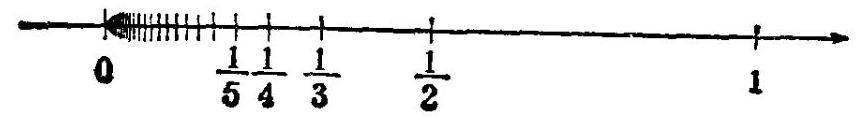
\includegraphics[width=0.5\textwidth]{images/01912c18-5c3f-733d-b775-749ba9897a9d_4_159408.jpg}

\end{center}

\begin{center}
	(1)
\end{center}


\begin{center}
	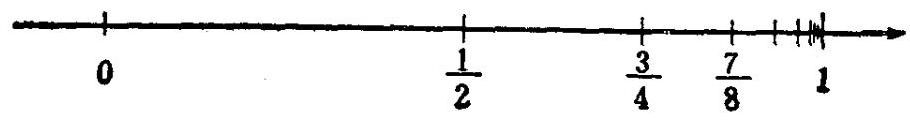
\includegraphics[width=0.5\textwidth]{images/01912c18-5c3f-733d-b775-749ba9897a9d_4_459236.jpg}
\end{center}

图 1-1

容易看出,当项数 \(n\) 无限增大时,数列 (1) 中的项无限趋近于 0 , 数列 (2) 中的项无限趋近于 1 .

事实上, 在数列 (1) 中, 各项与 0 的差的绝对值如下页的表所示.

我们看到,无论预先指定多么小的一个正数 \(\varepsilon\) ,总能在

\begin{center}
	\adjustbox{max width=\textwidth}{
		\begin{tabular}{|c|c|c|}
			\hline
			项 号 & 项 & 这一项与 0 的差的绝对值 \\
			\hline
			1 & 1 & \(\left| {0 - 1}\right| = 1\) \\
			\hline
			2 & \(\frac{1}{2}\) & \(\left| {0 - \frac{1}{2}}\right| = \frac{1}{2}\) \\
			\hline
			3 & \(\frac{1}{3}\) & \(\left| {0 - \frac{1}{3}}\right| = \frac{1}{3}\) \\
			\hline
			4 & \(\frac{1}{4}\) & \(\left| {0 - \frac{1}{4}}\right| = \frac{1}{4}\) \\
			\hline
			5 & \(\frac{1}{5}\) & \(\left| {0 - \frac{1}{5}}\right| = \frac{1}{5}\) \\
			\hline
			6 & \(\frac{1}{6}\) & \(\left| {0 - \frac{1}{6}}\right| = \frac{1}{6}\) \\
			\hline
			7 & \(\frac{1}{7}\) & \(\left| {0 - \frac{1}{7}}\right| = \frac{1}{7}\) \\
			\hline
			... & \(\cdots\) & \(\cdots\) \\
			\hline
		\end{tabular}
	}
\end{center}

数列 (1) 中找到这样一项, 使得这一项后面的所有项与 0 的差的绝对值都小于 \(\varepsilon\) . 例如,如果取 \(\varepsilon = \frac{1}{5}\) ,那么数列 (1) 中第 5 项后面所有的项与 0 的差的绝对值都小于 \(\varepsilon\) . 如果取 \(\varepsilon = \frac{1}{100}\) , 那么数列 (1) 中第 100 项后面所有的项与 0 的差的绝对值都小于 \(\varepsilon\) . 在这种情况下,我们就说数列 (1) 的极限是 0 .

同样, 对于数列 (2), 我们也可以列成下页的表.

可以看出,如果取 \(\varepsilon = {0.1}\) ,那么数列 (2) 中第 3 项后面所有的项与 1 的差的绝对值都小于 \(\varepsilon\) ; 如果取 \(\varepsilon = {0.01}\) ,那么第 6 项后面所有的项与 1 的差的绝对值都小于 \(\varepsilon\) . 就是说,无论预先指定多么小的一个正数 \(\varepsilon\) ,总能在数列(2)中找到这样一

\begin{center}
	\adjustbox{max width=\textwidth}{
		\begin{tabular}{|c|c|c|}
			\hline
			项 号 & 项 & 这一项与 1 的差的绝对值 \\
			\hline
			1 & \(\frac{1}{2}\) & \(\left| {\frac{1}{2} - 1}\right| = \frac{1}{2} = {0.5}\) \\
			\hline
			2 & \(\frac{3}{4}\) & \(\left| {\frac{3}{4} - 1}\right| = \frac{1}{4} = {0.25}\) \\
			\hline
			3 & \(\frac{7}{8}\) & \(\left| {\frac{7}{8} - 1}\right| = \frac{1}{8} = {0.125}\) \\
			\hline
			4 & \(\frac{15}{16}\) & \(\left| {\frac{15}{16} - 1}\right| = \frac{1}{16} = {0.0625}\) \\
			\hline
			5 & \(\frac{31}{32}\) & \(\left| {\frac{31}{32} - 1}\right| = \frac{1}{32} = {0.03125}\) \\
			\hline
			6 & \(\frac{63}{64}\) & \(\left| {\frac{63}{64} - 1}\right| = \frac{1}{64} = {0.015625}\) \\
			\hline
			7 & \(\frac{127}{128}\) & \(\left| {\frac{127}{128} - 1}\right| = \frac{1}{128} = {0.0078125}\) \\
			\hline
			\(\cdots\) & \(\cdots\) & \(\cdots\) \\
			\hline
		\end{tabular}
	}
\end{center}

项,使得这一项后面的所有项与 1 的差的绝对值都小于 \(\varepsilon\) . 这时, 我们说数列 (2) 的极限是 1 .

一般地,对于一个无穷数列 \(\left\{ {a}_{n}\right\}\) ,如果存在一个常数 \(A\) , 无论预先指定多么小的正数 \(\varepsilon\) ,都能在数列中找到一项 \({a}_{N}\) ,使得这一项后面所有的项与 \(A\) 的差的绝对值都小于 \(\varepsilon\) (即当 \(n >\) \(N\) 时, \(\left| {{a}_{n} - A}\right| < \varepsilon\) 恒成立),就把常数 \(A\) 叫做数列 \(\left\{ {a}_{n}\right\}\) 的极限, 记作

\[
\mathop{\lim }\limits_{{n \rightarrow \infty }}{a}_{n} = A\text{. O }
\]

这个式子读作 “当 \(n\) 趋向于无穷大时, \({a}_{n}\) 的极限等于 \({A}^{n}\) . “->” 表示 “趋向于”, “ \(\infty\) ” 表示 “无穷大”, “ \(n \rightarrow \infty\) ” 表示 “ \(n\) 趋向于无穷大”,也就是 \(n\) 无限增大的意思.

\customfootnote{
	
	O lim 是拉丁文 limis (极限) 一词的前三个字母, 一般按英文 limit (极限) 一词读音. \(\mathop{\lim }\limits_{{n \rightarrow \infty }}{a}_{n} = A\) 也可读作 “limit \({a}_{n}\) 当 \(n\) 趋于无穷大时等于 \({A}^{n}\) .
	
}

\(\mathop{\lim }\limits_{{n \rightarrow \infty }}{a}_{n} = A\) 有时也可记作

\[
\text{当}n \rightarrow \infty \text{时,}{a}_{n} \rightarrow A\text{.}
\]

从数列极限的定义可以看出,数列 \(\left\{ {a}_{n}\right\}\) 以 \(A\) 为极限,是指当 \(n\) 无限增大时,数列 \(\left\{ {a}_{n}\right\}\) 中的项 \({a}_{n}\) 无限趋近于常数 \(A\) .

例 1 已知数列

\[
1, - \frac{1}{2},\frac{1}{3}, - \frac{1}{4},\cdots ,{\left( -1\right) }^{n + 1}\frac{1}{n},\cdots \text{.}
\]

(1) 写出这个数列的各项与 0 的差的绝对值.

(2)第几项后面所有的项与 0 的差的绝对值都小于 0.1 ? 都小于 0.001 ? 都小于 0.0003 ?

(3)第几项后面所有的项与 0 的差的绝对值都小于任何预先指定的正数 \(\varepsilon\) ?

(4) 0 是不是这个数列的极限?

解: 这个数列的项在数轴上的表示如图 1-2:

\begin{center}
	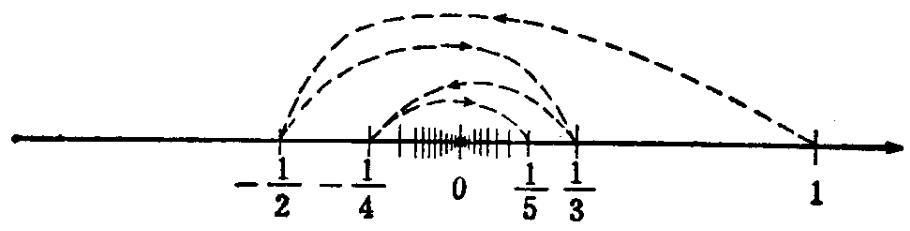
\includegraphics[max width=0.9\textwidth]{images/01912c18-5c3f-733d-b775-749ba9897a9d_7_608223.jpg}
\end{center}

图 1-2

(1)这个数列的各项与 0 的差的绝对值依次是

\[
1,\frac{1}{2},\frac{1}{3},\cdots ,\frac{1}{n},\cdots
\]

(2)要使 \(\frac{1}{n} < {0.1}\) ,只要 \(n > {10}\) 就行了. 这就是说,第 10 项后面所有的项与 0 的差的绝对值都小于 0.1 .

要使 \(\frac{1}{n} < {0.001}\) ,只要 \(n > {1000}\) 就行了. 这就是说,第 1000 项后面所有的项与 0 的差的绝对值都小于 0.001 .

要使 \(\frac{1}{n} < {0.0003}\) ,只要 \(n > {3333}\frac{1}{3}\) 就行了. 这就是说,第 3333 项后面所有的项与 0 的差的绝对值都小于 0.0003 .

(3)要使 \(\frac{1}{n} < \varepsilon\) ,只要 \(n > \frac{1}{\varepsilon }\) 就行了,因为所求的项数必须是正整数,因此设 \(\frac{1}{e}\) 的整数部分是 \(N\) ,那么第 \(N\) 项后面所有的项与 0 的差的绝对值都小于 \(\varepsilon\) .

(4)从(3)可以知道, 0 是这个数列的极限, 记作:

\[
\mathop{\lim }\limits_{{n \rightarrow \infty }}{\left( -1\right) }^{n + 1}\frac{1}{n} = 0
\]

例 2 已知数列

\[
\frac{1}{2},\frac{2}{3},\frac{3}{4},\cdots ,\frac{n}{n + 1},\cdots
\]

(1) 计算 \(\left| {{a}_{n} - 1}\right|\) .

(2)第几项后面所有的项与 1 的差的绝对值都小于 \(\frac{1}{100}\) ?

(3)第几项后面所有的项与 1 的差都小于任意指定的正数 \({\varepsilon }_{2}\)

(4) 1 是不是这个数列的极限?

解: (1) \(\left| {{a}_{n} - 1}\right| = \left| {\frac{n}{n + 1} - 1}\right| = \left| \frac{-1}{n + 1}\right| = \frac{1}{n + 1}\) .

(2)要使 \(\frac{1}{n + 1} < \frac{1}{100}\) ,就是要使 \(n + 1 > {100}\) ,即 \(n > {99}\) ,这就是说,第 99 项后面所有的项与 1 的差的绝对值都小于 \(\frac{1}{100}\) .

(3)要使 \(\frac{1}{n + 1} < \varepsilon\) ,就是要使 \(n + 1 > \frac{1}{\varepsilon }\) ,即 \(n > \frac{1}{\varepsilon } - 1\) ,设 \(\frac{1}{\varepsilon } - 1\) 的整数部分是 \(N\) ,那么第 \(N\) 项后面所有的项与 1 的差的绝对值都小于正数 \(\varepsilon\) .

(4) 从 (3) 可以知道, 这个数列的极限是 1 , 记作:

\[
\mathop{\lim }\limits_{{n \rightarrow \infty }}\frac{n}{n + 1} = 1
\]

例 3 已知数列

\[
\frac{1}{2},\frac{1}{4},\frac{1}{8},\cdots ,\frac{1}{{2}^{n}}\cdots
\]

(1) 计算 \(\left| {{a}_{n} - 0}\right|\) .

(2)第几项后面所有的项与 0 的差的绝对值小于正数 \(\varepsilon\) ?

(3) 0 是不是这个数列的极限?

解: (1) \(\left| {{a}_{n} - 0}\right| = \left| {\frac{1}{{2}^{n}} - 0}\right| = \frac{1}{{2}^{n}}\) .

(2)要使 \(\frac{1}{{2}^{n}} < \varepsilon\) ,就是要使 \(n > \frac{\ln \frac{1}{\varepsilon }}{\ln 2}\) . 设 \(\frac{\ln \frac{1}{\varepsilon }}{\ln 2}\) 的整数部分是 \(N\) ,那么第 \(N\) 项后面所有的项与 0 的差的绝对值都小于正数 \(\varepsilon\) .

(3)从 \(\left( 2\right)\) 可以知道,这个数列的极限是 0 ,记作

\[
\mathop{\lim }\limits_{{n \rightarrow \infty }}\frac{1}{{2}^{n}} = 0
\]

例 4 求常数数列 \(- 7, - 7, - 7,\cdots\) 的极限.

解: 这个数列的各项与 -7 的差的绝对值都等于 0 , 所以从第 1 项起,这个绝对值就能够小于任意指定的正数 \(\varepsilon\) ,因此这个数列的极限是 -7 .

一般地, 任何一个常数数列的极限都是这个常数本身, 即

\[
\mathop{\lim }\limits_{{n \rightarrow \infty }}C = C\text{ ( }C\text{ 是常数). }
\]

应该指出, 并不是每一个无穷数列都有极限. 例如, 数列

\[
1,2,3,\cdots ,n,\cdots
\]

就没有极限.

数列

\[
- 1,1, - 1,1,\cdots ,{\left( -1\right) }^{n},\cdots
\]

也没有极限.

\begin{problemset}[练习]
	\item 已知数列
	
	\[
	\frac{1}{{1}^{2}},\frac{1}{{2}^{2}},\frac{1}{{3}^{2}},\frac{1}{{4}^{2}},\cdots ,\frac{1}{{n}^{2}},\cdots
	\]
	
	(1)把这个数列的前 5 项在数轴上表示出来。
	
	(2)写出这个数列的各项与 0 的差的绝对值。
	
	(3)第几项后面的所有项与 0 的差的绝对值都小于 0.1 ? 都小于 0.01 ? 都小于 0.00011 都小于任何预先指定的正数 \(\varepsilon\) ?
	
	(4)是不是这个无穷数列的极限?
	
	\item 已知数列 \(4 - \frac{1}{10},4 - \frac{1}{20},4 - \frac{1}{30},\cdots ,4 - \frac{1}{10n},\cdots\) .
	
	(1) 计算 \(\left| {{a}_{n} - 4}\right|\) .
	
	(2) 第几项后面的所有项与 4 的差的绝对值都小于 0.01 ? 都小于任意指定的正数 \(\varepsilon\) ?
	
	(3) 确定这个数列的极限。
\end{problemset}



\section{数列极限的四则运算}
前面我们看到, 一些简单的数列可以从变化趋势找出它们的极限. 例如,

\[
\mathop{\lim }\limits_{{n \rightarrow \infty }}\frac{1}{n} = 0,\;\mathop{\lim }\limits_{{n \rightarrow \infty }}\frac{1}{{2}^{n}} = 0,\;\mathop{\lim }\limits_{{n \rightarrow \infty }}C = C.
\]

如果求极限的数列比较复杂, 就要分析已知数列是由哪些简单的数列经过怎样的运算结合而成的, 这样就能把复杂的数列的极限的计算问题转化为简单的数列的极限的计算问题. 因此, 下面引入数列极限的四则运算法则 (证明从略):

\[
\text{如果}\mathop{\lim }\limits_{{n \rightarrow \infty }}{a}_{n} = A,\mathop{\lim }\limits_{{n \rightarrow \infty }}{b}_{n} = B\text{,那么,}
\]

\[
\mathop{\lim }\limits_{{n \rightarrow \infty }}\left( {{a}_{n} \pm {b}_{n}}\right) = A \pm B
\]

\[
\mathop{\lim }\limits_{{n \rightarrow \infty }}\left( {{a}_{n} \cdot {b}_{n}}\right) = A \cdot B
\]

\[
\mathop{\lim }\limits_{{n \rightarrow \infty }}\frac{{a}_{n}}{{b}_{n}} = \frac{A}{B}\left( {B \neq 0}\right) .
\]

特别地,如果 \(C\) 是常数,那么,

\[
\mathop{\lim }\limits_{{n \rightarrow \infty }}\left( {C \cdot {a}_{n}}\right) = \mathop{\lim }\limits_{{n \rightarrow \infty }}C \cdot \mathop{\lim }\limits_{{n \rightarrow \infty }}{a}_{n} = {CA}.
\]

上面的数列极限的四则运算法则表明: 如果两个数列都有极限, 那么, 这两个数列的各对应项的和、差、积、商组成的数列的极限, 分别等于这两个数列的极限的和、差、积、商 (各项作为除数的数列的极限不能为零).

例如, 数列

\[
\frac{1}{2},\frac{2}{3},\frac{3}{4},\cdots ,\frac{n}{n + 1},\cdots
\]

与

\[
2,2,2,\cdots ,2,\cdots
\]

的极限分别是 1 与 2 , 那么根据上面的运算法则, 这两个数列的各对应项的和组成的数列

\[
2 + \frac{1}{2},2 + \frac{2}{3},2 + \frac{3}{4},\cdots ,2 + \frac{n}{n + 1},\cdots
\]

的极限是 3 .

例 1 已知 \(\mathop{\lim }\limits_{{n \rightarrow \infty }}{a}_{n} = 5,\mathop{\lim }\limits_{{n \rightarrow \infty }}{b}_{n} = 3\) ,求 \(\mathop{\lim }\limits_{{n \rightarrow \infty }}\left( {3{a}_{n} - 4{b}_{n}}\right)\) .

解: \(\mathop{\lim }\limits_{{n \rightarrow \infty }}\left( {3{a}_{n} - 4{b}_{n}}\right) = \mathop{\lim }\limits_{{n \rightarrow \infty }}3{a}_{n} - \mathop{\lim }\limits_{{n \rightarrow \infty }}4{b}_{n}\)

\[
= 3\mathop{\lim }\limits_{{n \rightarrow \infty }}{a}_{n} - 4\mathop{\lim }\limits_{{n \rightarrow \infty }}{b}_{n} = 3 \times 5 - 4 \times 3 = 3\text{.}
\]

例 2 求:

(1) \(\mathop{\lim }\limits_{{n \rightarrow \infty }}\left( {5 + \frac{1}{n}}\right)\) (2) \(\mathop{\lim }\limits_{{n \rightarrow \infty }}\frac{{3n} - 2}{n}\)

(3) \(\mathop{\lim }\limits_{{n \rightarrow \infty }}\frac{{2n} + 1}{{3n} + 2}\) (4) \(\mathop{\lim }\limits_{{n \rightarrow \infty }}\frac{3{n}^{2} - {2n} + 8}{4 - {n}^{2}}\) .

解: (1) \(\mathop{\lim }\limits_{{n \rightarrow \infty }}\left( {5 + \frac{1}{n}}\right) = \mathop{\lim }\limits_{{n \rightarrow \infty }}5 + \mathop{\lim }\limits_{{n \rightarrow \infty }}\frac{1}{n}\)

\[
= 5 + 0 = 5\text{. }
\]

(2) \(\mathop{\lim }\limits_{{n \rightarrow \infty }}\frac{{3n} - 2}{n} = \mathop{\lim }\limits_{{n \rightarrow \infty }}\left( {\frac{3n}{n} - \frac{2}{n}}\right)\)

\[
= \mathop{\lim }\limits_{{n \rightarrow \infty }}3 - \mathop{\lim }\limits_{{n \rightarrow \infty }}\left( {2 \cdot \frac{1}{n}}\right) = 3 - 2\mathop{\lim }\limits_{{n \rightarrow \infty }}\frac{1}{n}
\]

\[
= 3 - 2 \times 0 = 3\text{. }
\]

(3)当 \(n\) 无限增大时,分式 \(\frac{{2n} + 1}{{3n} + 2}\) 中的分子、分母同时无限增大, 上面的极限运算法则不能直接运用. 为此, 我们将分式中的分子、分母同时除以 \(n\) 后求它的极限,得

\[
\mathop{\lim }\limits_{{n \rightarrow \infty }}\frac{{2n} + 1}{{3n} + 2} = \mathop{\lim }\limits_{{n \rightarrow \infty }}\frac{2 + \frac{1}{n}}{3 + \frac{2}{n}}
\]

\[
= \frac{\mathop{\lim }\limits_{{n \rightarrow \infty }}\left( {2 + \frac{1}{n}}\right) }{\mathop{\lim }\limits_{{n \rightarrow \infty }}\left( {3 + \frac{2}{n}}\right) } = \frac{\mathop{\lim }\limits_{{n \rightarrow \infty }}2 + \mathop{\lim }\limits_{{n \rightarrow \infty }}\frac{1}{n}}{\mathop{\lim }\limits_{{n \rightarrow \infty }}3 + \mathop{\lim }\limits_{{n \rightarrow \infty }}\frac{2}{n}}
\]

\[
= \frac{2 + 0}{3 + 0} = \frac{2}{3}
\]

(4) \(\mathop{\lim }\limits_{{n \rightarrow \infty }}\frac{3{n}^{2} - {2n} + 8}{4 - {n}^{2}} = \mathop{\lim }\limits_{{n \rightarrow \infty }}\frac{3 - \frac{2}{n} + \frac{8}{{n}^{2}}}{\frac{4}{{n}^{2}} - 1}\)

\[
= \frac{\mathop{\lim }\limits_{{n \rightarrow \infty }}\left( {3 - \frac{2}{n} + \frac{8}{{n}^{2}}}\right) }{\mathop{\lim }\limits_{{n \rightarrow \infty }}\left( {\frac{4}{{n}^{2}} - 1}\right) } = \frac{\mathop{\lim }\limits_{{n \rightarrow \infty }}3 - \mathop{\lim }\limits_{{n \rightarrow \infty }}\frac{2}{n} + \mathop{\lim }\limits_{{n \rightarrow \infty }}\frac{8}{{n}^{2}}}{\mathop{\lim }\limits_{{n \rightarrow \infty }}\frac{4}{{n}^{2}} - \mathop{\lim }\limits_{{n \rightarrow \infty }}1}.
\]

\[
= \frac{3 - 0 + 0}{0 - 1} = - 3\text{. }
\]

例 3 已知等比数列

\[
\frac{1}{2},\frac{1}{4},\frac{1}{8},\cdots ,\frac{1}{{2}^{n}},\cdots
\]

求这个数列前 \(n\) 项的和当 \(n \rightarrow \infty\) 时的极限.

解: 这个等比数列的公比是

\[
q = \frac{\frac{1}{4}}{\frac{1}{2}} = \frac{1}{2}.
\]

根据等比数列前 \(n\) 项和的公式,得

\[
{S}_{n} = \frac{{a}_{1}\left( {1 - {q}^{n}}\right) }{1 - q} = \frac{\frac{1}{2}\left\lbrack {1 - {\left( \frac{1}{2}\right) }^{n}}\right\rbrack }{1 - \frac{1}{2}} = 1 - \frac{1}{{2}^{n}}.
\]

因此,

\[
\mathop{\lim }\limits_{{n \rightarrow \infty }}{S}_{n} = \mathop{\lim }\limits_{{n \rightarrow \infty }}\left( {1 - \frac{1}{{2}^{n}}}\right)
\]

\[
= 1 - \mathop{\lim }\limits_{{n \rightarrow \infty }}\frac{1}{{2}^{n}}
\]

\[
= 1 - 0 = 1\text{. }
\]

\begin{center}
	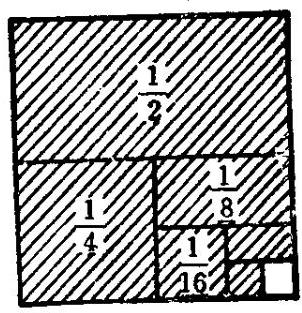
\includegraphics[max width=0.3\textwidth]{images/01912c18-5c3f-733d-b775-749ba9897a9d_14_791114.jpg}
\end{center}

图 1-3

上述结果可从图 1-3 中看出, 图 1-3 中各小矩形与小正

方形面积的和 (阴影部分) 的极限等于大正方形的面积.

例 3 中的无穷等比数列有这样的特点: 它的公比的绝对值小于 1 .

一般地, 设无穷等比数列

\[
{a}_{1},{a}_{1}q,{a}_{1}{q}^{2},\cdots ,{a}_{1}{q}^{n - 1},\cdots
\]

的公比 \(q\) 的绝对值小于 1,我们来求它的前 \(n\) 项的和当 \(n\) 无限增大时的极限.

无穷等比数列前 \(n\) 项的和是

\[
{S}_{n} = {a}_{1} + {a}_{1}q + \cdots + {a}_{1}{q}^{n - 1} = \frac{{a}_{1}\left( {1 - {q}^{n}}\right) }{1 - q},
\]

因此,

\[
\mathop{\lim }\limits_{{n \rightarrow \infty }}{S}_{n} = \mathop{\lim }\limits_{{n \rightarrow \infty }}\frac{{a}_{1}\left( {1 - {q}^{n}}\right) }{1 - q}
\]

\[
= \mathop{\lim }\limits_{{n \rightarrow \infty }}\frac{{a}_{1}}{1 - q} \cdot \mathop{\lim }\limits_{{n \rightarrow \infty }}\left( {1 - {q}^{n}}\right)
\]

\[
= \frac{{a}_{1}}{1 - q}\left( {\mathop{\lim }\limits_{{n \rightarrow \infty }}1 - \mathop{\lim }\limits_{{n \rightarrow \infty }}{q}^{n}}\right) .
\]

因为当 \(\left| q\right| < 1\) 时, \(\mathop{\lim }\limits_{{n \rightarrow \infty }}{q}^{n} = 0\) (证明较繁,本书从略),所以,

\[
\mathop{\lim }\limits_{{n \rightarrow \infty }}{S}_{n} = \frac{{a}_{1}}{1 - q} \cdot \left( {1 - 0}\right) = \frac{{a}_{1}}{1 - q}.
\]

公比的绝对值小于 1 的无穷等比数列前 \(n\) 项的和当 \(n\) 无限增大时的极限, 叫做这个无穷等比数列各项的和(注意: 这与有限个数的和从意义上说是不一样的),并且用符号 \(S\) 表示. 从上面知道,

\[
S = {a}_{1} + {a}_{1}q + {a}_{1}{q}^{2} + \cdots + {a}_{1}{q}^{n - 1} + \cdots = \frac{{a}_{1}}{1 - q}.
\]

例 4 求无穷等比数列 \({0.3},{0.03},{0.003},\cdots\) 各项的和.

解: \(\because {a}_{1} = {0.3},q = {0.1}\) ,

\[
\therefore \;S = \frac{0.3}{1 - {0.1}} = \frac{1}{3}\text{. }
\]

例 5 将下列循环小数化成分数:

(1) 0.7 ; (2) 0.231 .

解: (1) 纯循环小数 \({0.7} = {0.777}\cdots\) 可以写成

\[
\frac{7}{10} + \frac{7}{100} + \frac{7}{1000} + \cdots
\]

这里各项组成公比等于 \(\frac{1}{10}\) 的无穷等比数列,因此,

\[
{0.7} = \frac{\frac{7}{10}}{1 - \frac{1}{10}} = \frac{\frac{7}{10}}{\frac{9}{10}} = \frac{7}{9}
\]

也就是说, \({0.7} = \frac{7}{9}\) .

(2)混循环小数 \({0.231} = {0.2313131}\cdots\) 可以写成

\[
\frac{2}{10} + \frac{31}{1000} + \frac{31}{100000} + \frac{31}{10000000} + \cdots ,
\]

这里从第 2 项起各项组成公比等于 \(\frac{1}{100}\) 的无穷等比数列, 因此,

\[
{0.2}\dot{3}\dot{1} = \frac{2}{10} + \frac{\frac{31}{1000}}{1 - \frac{1}{100}} = \frac{2}{10} + \frac{31}{990}
\]

\[
= \frac{2 \times {99} + {31}}{990} = \frac{229}{990}
\]

\begin{problemset}[练习]
\item 已知 \(\mathop{\lim }\limits_{{n \rightarrow \infty }}{a}_{n} = 2,\mathop{\lim }\limits_{{n \rightarrow \infty }}{b}_{n} = - \frac{1}{3}\) ,求下列极限:

(1) \(\mathop{\lim }\limits_{{n \rightarrow \infty }}\left( {2{a}_{n} + 3{b}_{n}}\right)\) ; (2) \(\mathop{\lim }\limits_{{n \rightarrow \infty }}\frac{{a}_{n} - {b}_{n}}{{a}_{n}}\) .

\item 求下列极限:

(1) \(\mathop{\lim }\limits_{{n \rightarrow \infty }}\left( {3 - \frac{1}{n}}\right)\) (2) \(\mathop{\lim }\limits_{{n \rightarrow \infty }}\frac{2}{5 + \frac{3}{n}}\)

(3) \(\mathop{\lim }\limits_{{n \rightarrow \infty }}\frac{n + 1}{n}\) (4) \(\mathop{\lim }\limits_{{n \rightarrow \infty }}\frac{n - 1}{{n}^{2} + 1}\) .

\item 求下列无穷等比数列各项的和:

(1) \(3,1,\frac{1}{3},\frac{1}{9},\cdots\) ; (2) \(1, - \frac{1}{2},\frac{1}{4}, - \frac{1}{8},\cdots\) .

\end{problemset}
\begin{problemset}[习题一]
	\item 已知无穷数列 \(5 + 1,5 - \frac{1}{2},5 + \frac{1}{3},5 - \frac{1}{4},\cdots\) .
	
	(1)把这个数列的前 5 项在数轴上表示出来.
	
	(2)计算这个数列的第 \(n\) 项与 5 的差的绝对值 \(\left| {{a}_{n} - 5}\right|\) .
	
	(3)对于任何预先指定的正数 \(\varepsilon\) ,找一个自然数 \(N\) ,使得 \(n > N\) 时, \(\left| {{a}_{n} - 5}\right| < \varepsilon\) .
	
	(4)确定这个数列的极限。
	
	\item 一个无穷数列的通项公式是 \({a}_{n} = \frac{n + 1}{n + 2}\) .
	
	(1)把这个数列的前 5 项在数轴上表示出来。
	
	(2)计算 \(\left| {{a}_{n} - 1}\right|\) .
	
	(3)对于下表中的 \(\varepsilon\) ,各找出一个对应的自然数 \(N\) ,使得 \(n > N\) 时, \(\left| {{a}_{n} - 1}\right| < \varepsilon\) .
	
	\begin{center}
		\adjustbox{max width=\textwidth}{
			\begin{tabular}{|c|c|c|c|c|c|}
				\hline
				e & 0.2 & 0.1 & 0.05 & 0.01 & 任何给定 的正数 \\
				\hline
				\(N\) & \phantom{X} & \phantom{X} & \phantom{X} & \phantom{X} & \phantom{X} \\
				\hline
			\end{tabular}
		}
	\end{center}
	
	(4)确定这个数列的极限.
	
	\item 一个无穷数列的通项公式是 \({a}_{n} = \frac{{8n} + 1}{2n}\) .
	
	(1)把这个数列的前 5 项在数轴上表示出来.
	
	(2)计算 \(\left| {{a}_{n} - 4}\right|\) .
	
	(3)确定这个无穷数列的极限。
	
	\item 一个无穷数列的通项公式是 \({a}_{n} = \frac{n}{{2n} + 1}\) ,求证这个数列的极限是 \(\frac{1}{2}\) 。
	
	\item 举一个极限是 5 的无穷数列的例子.
	
	\item 无穷数列 \(- 2,0, - 2,0,\cdots ,{\left( -1\right) }^{n} - 1,\cdots\) 有极限吗?
	
	\item 已知无穷数列
	
	\[
	\frac{5}{3},\frac{10}{4},\frac{15}{5},\cdots ,\frac{5n}{n + 2},\cdots
	\]
	
	\[
	\frac{1}{3},\frac{2}{4},\frac{3}{5},\cdots ,\frac{n}{n + 2},\cdots
	\]
	
	(1)求证这两个数列的极限分别是 5 与 1 .
	
	(2)另作一个每一项都等于这两个数列的对应项的和的无穷数列. 验证所得数列的极限等于这两个数列的极限的和。
	
	\item 求下列极限:
	
	(1) \(\mathop{\lim }\limits_{{n \rightarrow \infty }}\left( {\frac{3}{{n}^{2}} + \frac{1}{n} + 5}\right)\) ; (2) \(\mathop{\lim }\limits_{{n \rightarrow \infty }}\frac{{2n} + 1}{{2n} - 1}\)
	
	(3) \(\mathop{\lim }\limits_{{n \rightarrow \infty }}\left( {\frac{2}{n} + \frac{{4n} - 1}{4n}}\right)\) (4) \(\mathop{\lim }\limits_{{n \rightarrow \infty }}\left( {1 - \frac{2n}{n + 2}}\right)\) ;
	
	(5) \(\mathop{\lim }\limits_{{n \rightarrow \infty }}\frac{5 + {7n}}{{6n} - {11}}\) (6) \(\mathop{\lim }\limits_{{n \rightarrow \infty }}\frac{2{n}^{2} + n - 1}{3{n}^{2} - 1}\)
	
	(7) \(\mathop{\lim }\limits_{{n \rightarrow \infty }}\frac{n + 1}{{n}^{2} - 9}\) (8) \(\mathop{\lim }\limits_{{n \rightarrow \infty }}\frac{{n}^{2} + n + 1}{{\left( n - 1\right) }^{2}}\) .
	
	\item (1) 求 \(\mathop{\lim }\limits_{{n \rightarrow \infty }}\frac{1 + 2 + \cdots + n}{{n}^{2}}\)
	
	(2)求 \(\mathop{\lim }\limits_{{n \rightarrow \infty }}\frac{{1}^{2} + {2}^{2} + \cdots + {n}^{2}}{{n}^{3}}\) .
	
	\[
	\text{(提示:}{1}^{2} + {2}^{2} + \cdots + {n}^{2} = \frac{n\left( {n + 1}\right) \left( {{2n} + 1}\right) }{6}\text{.}
	\]
	
	\item (1) 如图,在圆的内接正多边形中, \({r}_{n}\) 是边心距, \({p}_{n}\) 是周长, \({S}_{n}\) 是面积,求证 \({S}_{n} = \frac{1}{2}{p}_{n}{r}_{n}\) .
	
	(2)当圆的内接正多边形的边数无限增加时, \({r}_{n}\) 的极限是圆的半径 \(R,{p}_{n}\) 的极限是圆周长 \({2\pi R},{S}_{n}\) 的极限是圆面积,求证圆面积等于 \(\pi {R}^{2}\) .
	
	\item 如图,三角形的一条底边是 \(a\) ,这条边上的高是 \(h\) .
	
	(1)过高的 5 等分点分别作底边的平行线, 并作出相应的 4 个矩形, 求这些矩形面积的和.
	
	(2)把高 \(n\) 等分,同样作出 \(n - 1\) 个矩形,求这些矩形面积的和.
	
	(3)求证: 当 \(n\) 无限增大时,这些矩形面积的和的极限等于三角形的面积 \(\frac{ah}{2}\) .
	
	\begin{center}
		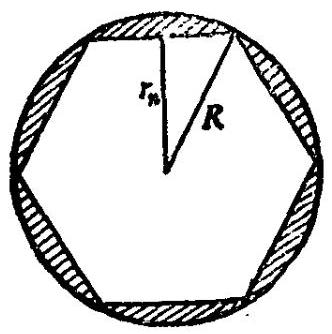
\includegraphics[max width=0.3\textwidth]{images/01912c18-5c3f-733d-b775-749ba9897a9d_20_155049.jpg}
	\end{center}
	
	(第 10 题)
	
	\begin{center}
		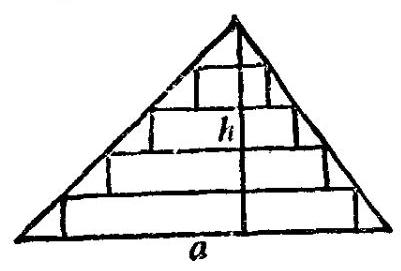
\includegraphics[max width=0.4\textwidth]{images/01912c18-5c3f-733d-b775-749ba9897a9d_20_862371.jpg}
	\end{center}
	
	(第 11 题)
	
	\item 求下列无穷等比数列各项的和:
	
	(1) \(\frac{8}{9}, - \frac{2}{3},\frac{1}{2}, - \frac{3}{8},\cdots\) ;
	
	(2) \(6\frac{2}{3},1\frac{1}{3},\frac{4}{15},\frac{4}{75},\cdots\) ;
	
	(3) \(\frac{\sqrt{3} + 1}{\sqrt{3} - 1},1,\frac{\sqrt{3} - 1}{\sqrt{3} + 1},\cdots\) ;
	
	(4) \(1, - x,{x}^{2}, - {x}^{3},\cdots ,\left( {\left| x\right| < 1}\right)\) .
	
	\item 如图,等边三角形 \({ABC}\) 的面积等于 1,连结这个三角形各边的中点得到一个小三角形, 又连结这个小三角形各边的中点得到一个更小的三角形, 如此无限继续下去, 求所有这些三角形面积的和。
	
	\begin{center}
		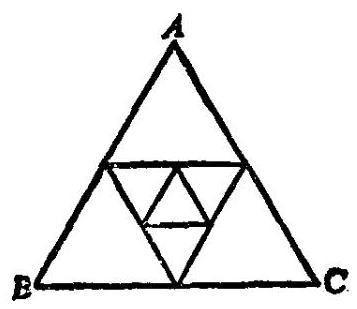
\includegraphics[max width=0.4\textwidth]{images/01912c18-5c3f-733d-b775-749ba9897a9d_20_529798.jpg}
	\end{center}
	
	(第 13 题)
	
	\begin{center}
		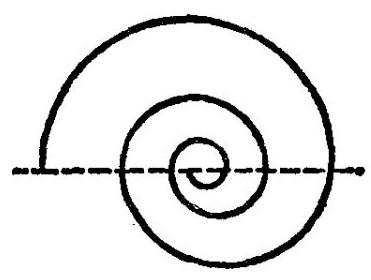
\includegraphics[max width=0.4\textwidth]{images/01912c18-5c3f-733d-b775-749ba9897a9d_20_500122.jpg}
	\end{center}
	
	(第 14 题)
	
	\item 如图, 第 1 个半圆的直径是 3 厘米, 第 2 个半圆的直径是
	
	2 厘米,以后每个半圆的直径都是前一个的 \(\frac{2}{3}\) ,这样无限继续下去, 求整条曲线的长。
	
	\item 将下列循环小数化成分数:
	
	(1) \({0.4}\) ; (2) 0.135 ;
	
	(3) \({0.436}\) ; (4) 2.138 .
	
\end{problemset}

\section{函数的极限}
前面我们研究了数列的极限的概念和极限的运算法则. 从本节起, 我们将讨论函数的极限的概念和运算法则.

\section*{1.当 \(x \rightarrow \infty\) 时函数的极限}


我们考察函数 \(y = \frac{1}{x}\) 当 \(x\) 无限增大时的变化趋势. 为此,

我们列出下表,并作出函数 \(y = \frac{1}{x}\) 的图象 (图 1-4).

\begin{center}
	\adjustbox{max width=\textwidth}{
		\begin{tabular}{|c|c|c|c|c|c|c|c|}
			\hline
			\(x\) & 1 & 10 & 100 & 1000 & 10000 & 100000 & 母曲曲 \\
			\hline
			\(y\) & 1 & 0.1 & 0.01 & 0.001 & 0.0001 & 0.00001 & ... \\
			\hline
		\end{tabular}
	}
\end{center}

从函数 \(y = \frac{1}{x}\) 的图象可以看出,当自变量 \(x\) 取正值并无限增大时,函数 \(y = \frac{1}{x}\) 的值无限趋近于零. 这里的“无限趋近于零”,就是表示函数值 \(y\) 与 0 之差的绝对值 \(\left| {y - 0}\right|\) 可以变得任意小.

\begin{center}
	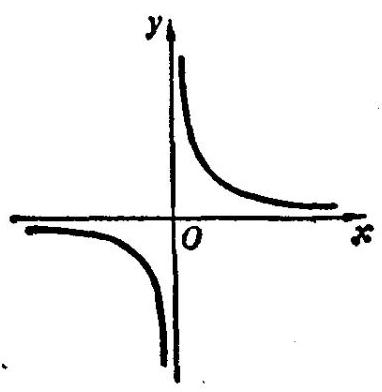
\includegraphics[max width=0.4\textwidth]{images/01912c18-5c3f-733d-b775-749ba9897a9d_21_654074.jpg}
\end{center}

图 1-4

例如,当 \(x\) 大于 1000 时,

\[
\left| {y - 0}\right| < {0.001}\text{.}
\]

当 \(x\) 大于 100000 时,

\[
\left| {y - 0}\right| < {0.00001}\text{.}
\]

一般地,对于预先指定的任意小的正数 \(\varepsilon\) ,当 \(x > \frac{1}{\varepsilon }\) 时,

\[
\left| {y - 0}\right| = \frac{1}{x} < \varepsilon
\]

总之,当 \(x\) 取正值并无限增大时,函数 \(y = \frac{1}{x}\) 的值无限趋近于 0 . 于是我们说,当 \(x\) 趋向于正无穷大时,函数 \(y = \frac{1}{x}\) 的极限是 0 , 记作

\[
\mathop{\lim }\limits_{{x \rightarrow + \infty }}\frac{1}{x} = 0
\]

同样地,当 \(x\) 取负值并且它的绝对值无限增大时,函数 \(y = \frac{1}{x}\) 的值也无限趋近于 0 . 于是我们说,当 \(x\) 趋向于负无穷大时,函数 \(y = \frac{1}{x}\) 的极限是 0,记作.

\[
\mathop{\lim }\limits_{{x \rightarrow - \infty }}\frac{1}{x} = 0
\]

一般地,当自变量 \(x\) 的绝对值无限增大时,如果函数 \(f\left( x\right)\) 无限趋近于一个常数 \(A\) ,就说当 \(x\) 趋向于无穷大时,函数 \(f\left( x\right)\) 的极限是 \(A\) ,记作

\[
\mathop{\lim }\limits_{{x \rightarrow \infty }}f\left( x\right) = A
\]

也可记作

当 \(x \rightarrow \infty\) 时, \(f\left( x\right) \rightarrow A\) .

\section*{2.当 \(x \rightarrow {x}_{0}\) 时函数的极限}


我们来研究函数 \(y = {x}^{2}\) 当 \(x\) 无限趋近于 2 时的变化趋势.

先列出下表,并作出函数 \(y = {x}^{2}\) 的图象 (图 1-5).

\begin{center}
	\adjustbox{max width=\textwidth}{
		\begin{tabular}{|c|c|c|c|c|c|c|}
			\hline
			\(x\) & 1. 5 & 1.9 & 1.99 & 1.999 & 1. 9999 & ... \\
			\hline
			\(y\) & 2. 25 & 3. 61 & 3.96 & 3.996 & 3 9996 & ... \\
			\hline
			\(\left| {y - 4}\right|\) & 1.75 & 0.39 & 0.04 & 0.004 & 0.0004 & es \\
			\hline
		\end{tabular}
	}
\end{center}

\begin{center}
	\adjustbox{max width=\textwidth}{
		\begin{tabular}{|c|c|c|c|c|c|c|}
			\hline
			\(x\) & 2. 5 & 2. 1 & 2.01 & 2.001 & 2.0001 & ... \\
			\hline
			\(y\) & 6.25 & 4.41 & 4.04 & 4.004 & 4.0004 & * \(* *\) \\
			\hline
			\(\left| {y - 4}\right|\) & 2. 25 & 0.41 & 0.04 & 0.004 & 0.0004 & . \\
			\hline
		\end{tabular}
	}
\end{center}

我们看到,当自变量 \(x\) 越接近 2 时,函数 \(y = {x}^{2}\) 的值越接近 4; 当 \(x\) 无限趋近于 2 (但不等于 2 ) 时, \(y\) 的值无限趋近于 4 . 于是我们说,当 \(x\) 无限趋近于 2 时,函数 \(y = {x}^{2}\) 的极限是 4,记作

\[
\mathop{\lim }\limits_{{x \rightarrow 2}}{x}^{2} = 4\text{. }
\]

\begin{center}
	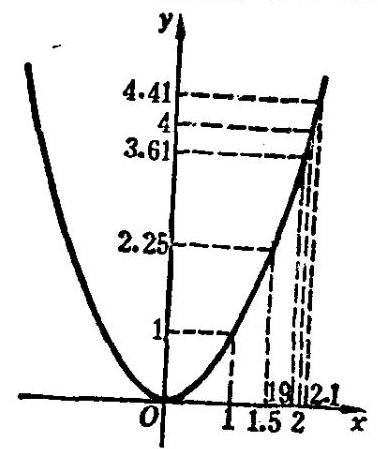
\includegraphics[max width=0.4\textwidth]{images/01912c18-5c3f-733d-b775-749ba9897a9d_23_174405.jpg}
\end{center}

图 1-5

我们再来研究函数 \(y = \frac{{x}^{2} - 1}{x - 1}\) 当 \(x\) 无限趋近于 1 (但不等 1)时的变化趋势.

如图 1-6,函数的图象是直线 \(y = x + 1\) 上除去点 \(\left( {1,2}\right)\) 以外的部分. 从图象上看到,当 \(x\) 接近于 1 时,函数 \(y = \frac{{x}^{2} - 1}{x - 1}\) 的值趋近于 2 .

\begin{center}
	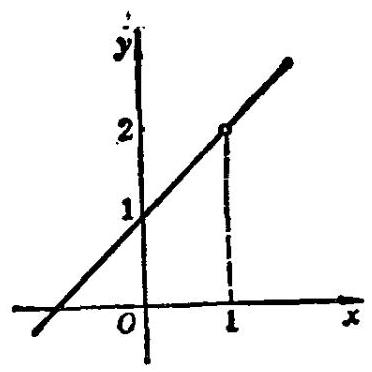
\includegraphics[max width=0.4\textwidth]{images/01912c18-5c3f-733d-b775-749ba9897a9d_24_728399.jpg}
\end{center}

图 1-6

这时,我们说,当 \(x\) 无限趋近于 1 (但不等于 1 ) 时, 函数

\[
y = \frac{{x}^{2} - 1}{x - 1}
\]

的极限是 2 , 记作

\[
\mathop{\lim }\limits_{{x \rightarrow 1}}\frac{{x}^{2} - 1}{x - 1} = 2
\]

一般地,当自变量 \(x\) 无限趋近于常数 \({x}_{0}\) (但 \(x\) 不等于 \({x}_{0}\) ) 时,如果函数 \(y = f\left( x\right)\) 无限趋近于一个常数 \(A\) ,就说当 \(x\) 趋近于 \({x}_{0}\) 时,函数 \(f\left( x\right)\) 的极限是 \(A\) ,记作

\[
\mathop{\lim }\limits_{{x \rightarrow {x}_{0}}}f\left( x\right) = A
\]

或者

当 \(x \rightarrow {x}_{0}\) 时, \(f\left( x\right) \rightarrow A\) .

从这个定义可以得出:

当 \(x\) 趋于任何数 \({x}_{0}\) 时,常数函数的极限就是这个常数, 即

\[
\mathop{\lim }\limits_{{x \rightarrow {x}_{0}}}C = C\text{. }
\]

当 \(x \rightarrow {x}_{0}\) 时, \(f\left( x\right) = x\) 的极限是 \({x}_{0}\) ,即

\[
\mathop{\lim }\limits_{{x \rightarrow {x}_{0}}}x = {x}_{0}
\]

\section*{3.函数的左极限和右极限}

首先,我们介绍在微积分中常常用到的函数 \(y = \left\lbrack x\right\rbrack\) ,符号 \(\left\lbrack x\right\rbrack\) 表示不超过数 \(x\) 的整数部分,例如

\[
\left\lbrack 0\right\rbrack = 0,\left\lbrack \frac{10}{3}\right\rbrack = \left\lbrack {{3.33}\cdots \cdots }\right\rbrack = 3,\;\left\lbrack {-{2.5}}\right\rbrack = - 3.
\]

函数 \(y = \left\lbrack x\right\rbrack\) 的图象如图 1-7.

现在,我们再来研究函数 \(y = \left\lbrack x\right\rbrack\) 在点 \(x = 1\) 处的极限.

如图 1-7,当 \(x\) 从点 \(x = 1\) 的左侧趋近于 1 时,函数 \(y\) 趋近于 0 ; 当 \(x\) 从点 \(x = 1\) 的右侧趋近于 1 时,函数 \(y\) 趋近于 1 . 因此,当 \(x\) 从点 \(x = 1\) 的左侧和右侧分别趋近于 1 时,函数 \(y\) 所趋近的值不同. 根据函数在一点处的极限的定义,函数 \(y\) 的极限不存在.

\begin{center}
	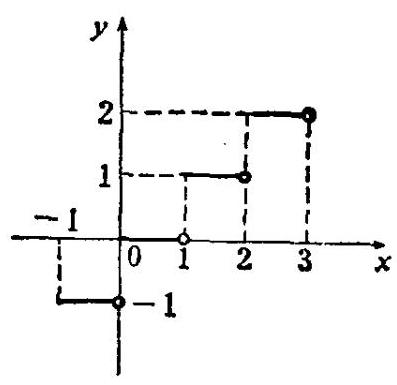
\includegraphics[max width=0.4\textwidth]{images/01912c18-5c3f-733d-b775-749ba9897a9d_25_214056.jpg}
\end{center}

图 1-7

从这个例子我们看到,虽然函数 \(y = \left\lbrack x\right\rbrack\) 在点 \(x = 1\) 处没有极限,但是当 \(x\) 从点 \(x = 1\) 的一侧趋近于 1 时,函数 \(y\) 还是趋近于确定的常数. 由此我们引出单侧极限的定义.

如果当 \(x\) 从点 \(x = {x}_{0}\) 左侧 (即 \(x < {x}_{0}\) ) 无限趋近于 \({x}_{0}\) 时,函数 \(f\left( x\right)\) 无限趋近于常数 \(A\) ,就说 \(A\) 是函数 \(f\left( x\right)\) 在点 \({x}_{0}\) 处的左极限, 记作

\[
\mathop{\lim }\limits_{{x \rightarrow {x}_{0} - }}f\left( x\right) = A\text{. }
\]

同样,如果当 \(x\) 从点 \(x = {x}_{0}\) 右侧 (即 \(x > {x}_{0}\) ) 无限趋近于 \({x}_{0}\) 时,函数 \(f\left( x\right)\) 无限趋近于常数 \(A\) ,就说 \(A\) 是函数 \(f\left( x\right)\) 在点 \({x}_{0}\) 处的右极限, 记作

\[
\mathop{\lim }\limits_{{x \rightarrow {x}_{0} + }}f\left( x\right) = A.
\]

根据极限、左极限和右极限的定义, 可以得出表示它们之间的关系的一条定理 (证明从略):

定理 \(\mathop{\lim }\limits_{{x \rightarrow {x}_{0}}}f\left( x\right) = A\) 的充要条件是

\[
\mathop{\lim }\limits_{{x \rightarrow {x}_{0} + }}f\left( x\right) = \mathop{\lim }\limits_{{x \rightarrow {x}_{0} - }}f\left( x\right) = A.
\]

\begin{problemset}[练习]
	\item 给定函数 \(y = \frac{1}{{x}^{2} + 1}\) . 填写下表并画出函数的图象,观察函数 \(y\) 当 \(x \rightarrow \infty\) 时的变化趋势:
	
	\begin{center}
		\adjustbox{max width=\textwidth}{
			\begin{tabular}{|c|c|c|c|c|c|c|}
				\hline
				\(x\) & 0 & \(\pm 2\) & \(\pm {10}\) & \(\pm {10}^{2}\) & \(\pm {10}^{3}\) & est \\
				\hline
				\(y\) & \phantom{X} & \phantom{X} & \phantom{X} & \phantom{X} & \phantom{X} & \phantom{X} \\
				\hline
				\(\left| {y - 0}\right|\) & \phantom{X} & \phantom{X} & \phantom{X} & \phantom{X} & \phantom{X} & \phantom{X} \\
				\hline
			\end{tabular}
		}
	\end{center}
	
	\item 根据函数极限的定义和函数的图象, 说出下列极限:
	
	(1) \(\mathop{\lim }\limits_{{x \rightarrow + \infty }}\frac{1}{{x}^{3}}\) (2) \(\mathop{\lim }\limits_{{x \rightarrow - \infty }}\frac{1}{{x}^{3}}\) (3) \(\mathop{\lim }\limits_{{x \rightarrow \infty }}\frac{1}{{x}^{3}}\) .
	
	\item 对于函数 \(y = {2x} + 1\) 填写下表,并作出函数的图象,观察当 \(x \rightarrow 1\) 时函数 \(y = {2x} + 1\) 的变化趋势:
	
	\begin{center}
		\adjustbox{max width=\textwidth}{
			\begin{tabular}{|c|c|c|c|c|c|c|}
				\hline
				\(x\) & 0.5 & 0.9 & 0.99 & 0.999 & 0.9999 & 0.99999 \\
				\hline
				\(y\) & \phantom{X} & \phantom{X} & \phantom{X} & \phantom{X} & \phantom{X} & \phantom{X} \\
				\hline
				\(\left| {y - 3}\right|\) & \phantom{X} & \phantom{X} & \phantom{X} & \phantom{X} & \phantom{X} & \phantom{X} \\
				\hline
			\end{tabular}
		}
	\end{center}
	
	\begin{center}
		\adjustbox{max width=\textwidth}{
			\begin{tabular}{|c|c|c|c|c|c|c|}
				\hline
				\(x\) & 1. 5 & 1. 1 & 1.01 & 1.001 & 1.0001 & 1.00001 \\
				\hline
				\(y\) & \phantom{X} & \phantom{X} & \phantom{X} & \phantom{X} & \phantom{X} & \phantom{X} \\
				\hline
				\(\left| {y - 3}\right|\) & \phantom{X} & \phantom{X} & \phantom{X} & \phantom{X} & \phantom{X} & \phantom{X} \\
				\hline
			\end{tabular}
		}
	\end{center}
	
	(1)当 \(\left| {x - 1}\right| < {0.01}\) 时, \(\left| {y - 3}\right|\) 小于什么数? 当 \(\left| {x - 1}\right|\) \(< {0.00001}\) 时, \(\left| {y - 3}\right|\) 小于什么数?
	
	(2)说出当 \(x \rightarrow 1\) 时函数 \(y\) 的极限.
	
	\item 根据函数极限的定义和函数的图象, 说出下列函数的极限 (其中 \(C\) 是常数):
	
	(1) \(\mathop{\lim }\limits_{{x \rightarrow \infty }}C\) ; (2) \(\mathop{\lim }\limits_{{x \rightarrow 3}}C\) ;
	
	(3) \(\mathop{\lim }\limits_{{x \rightarrow \infty }}\frac{1}{{x}^{2}}\) (4) \(\mathop{\lim }\limits_{{x \rightarrow 2}}\frac{1}{{x}^{2}}\) .
	
	\item 说出下列各图中表示的函数在点 \(x = a\) 的左极限、右极限和极限 (如果存在的话):
	
	\begin{center}
		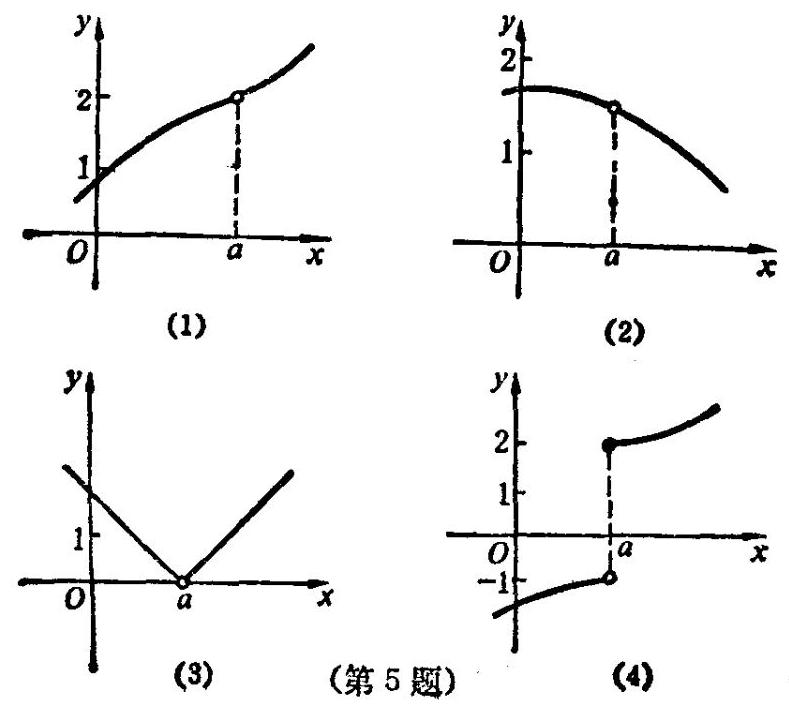
\includegraphics[max width=0.8\textwidth]{images/01912c18-5c3f-733d-b775-749ba9897a9d_27_586841.jpg}
	\end{center}
	
\end{problemset}

\section{函数极限的四则运算法则}

函数极限的四则运算与数列极限的四则运算有类似的定理.

如果 \(\mathop{\lim }\limits_{{x \rightarrow {x}_{0}}}f\left( x\right) = A,\mathop{\lim }\limits_{{x \rightarrow {x}_{0}}}g\left( x\right) = B\) ,那么,

\[
\mathop{\lim }\limits_{{x \rightarrow {x}_{0}}}\left\lbrack {f\left( x\right) \pm g\left( x\right) }\right\rbrack = A \pm B;
\]

\[
\mathop{\lim }\limits_{{x \rightarrow {x}_{0}}}\left\lbrack {f\left( x\right) \cdot \mathbf{g}\left( x\right) }\right\rbrack = \mathbf{A} \cdot \mathbf{B};
\]

\[
\mathop{\lim }\limits_{{x \rightarrow {x}_{0}}}\frac{f\left( x\right) }{g\left( x\right) } = \frac{A}{B}\left( {B \neq 0}\right) .
\]

这个定理对于 \(x \rightarrow \infty\) 的情况仍然成立.

由上面第二个式子可以推出: 当 \(C\) 是常数、 \(n\) 是正整数时,

\[
\mathop{\lim }\limits_{{x \rightarrow {x}_{0}}}\left\lbrack {{Cf}\left( x\right) }\right\rbrack = C\mathop{\lim }\limits_{{x \rightarrow {x}_{0}}}f\left( x\right) ;
\]

\[
\mathop{\lim }\limits_{{x \rightarrow {x}_{0}}}{\left\lbrack f\left( x\right) \right\rbrack }^{n} = {\left\lbrack \mathop{\lim }\limits_{{x \rightarrow {x}_{0}}}f\left( x\right) \right\rbrack }^{n}.
\]

利用函数极限的运算法则, 我们可以根据已知的几个函数的极限, 求出较复杂的函数的极限.

例 1 求 \(\mathop{\lim }\limits_{{x \rightarrow 2}}\left( {{x}^{2} + {3x}}\right)\) .

解: \(\mathop{\lim }\limits_{{x \rightarrow 2}}\left( {{x}^{2} + {3x}}\right) = \mathop{\lim }\limits_{{x \rightarrow 2}}{x}^{2} + \mathop{\lim }\limits_{{x \rightarrow 2}}{3x}\)

\[
= {\left( \mathop{\lim }\limits_{{x \rightarrow 2}}x\right) }^{2} + 3\mathop{\lim }\limits_{{x \rightarrow 2}}x
\]

\[
= {2}^{2} + 3 \times 2 = {10}\text{. }
\]

例 2 求 \(\mathop{\lim }\limits_{{x \rightarrow 1}}\frac{2{x}^{3} - {x}^{2} + 1}{x + 1}\) .

解: \(\mathop{\lim }\limits_{{x \rightarrow 1}}\frac{2{x}^{3} - {x}^{2} + 1}{x + 1} = \frac{\mathop{\lim }\limits_{{x \rightarrow 1}}\left( {2{x}^{3} - {x}^{2} + 1}\right) }{\mathop{\lim }\limits_{{x \rightarrow 1}}\left( {x + 1}\right) }\)

\[
= \frac{\mathop{\lim }\limits_{{x \rightarrow 1}}2{x}^{3} - \mathop{\lim }\limits_{{x \rightarrow 1}}{x}^{2} + \mathop{\lim }\limits_{{x \rightarrow 1}}1}{\mathop{\lim }\limits_{{x \rightarrow 1}}x + \mathop{\lim }\limits_{{x \rightarrow 1}}1}
\]

\[
= \frac{2{\left( \mathop{\lim }\limits_{{x \rightarrow 1}}x\right) }^{3} - {\left( \mathop{\lim }\limits_{{x \rightarrow 1}}x\right) }^{2} + \mathop{\lim }\limits_{{x \rightarrow 1}}1}{\mathop{\lim }\limits_{{x \rightarrow 1}}x + \mathop{\lim }\limits_{{x \rightarrow 1}}1}
\]

\[
= \frac{2 \times {1}^{3} - {1}^{2} + 1}{1 + 1}
\]

\[
= 1\text{.}
\]

例 3 求 \(\mathop{\lim }\limits_{{x \rightarrow 4}}\frac{{x}^{2} - {16}}{x - 4}\) .

分析: 当 \(x \rightarrow 4\) 时,分母的极限是 0,不能直接运用上面的极限运算法则. 因为当 \(x \rightarrow 4\) 时函数的极限,只与 \(x\) 无限趋近于 4 时的函数值有关,与 \(x = 4\) 时的函数值无关,因此可以先将分子和分母约去公因式 \(x - 4\) 以后再求函数的极限.

解: \(\mathop{\lim }\limits_{{x \rightarrow 4}}\frac{{x}^{2} - {16}}{x - 4} = \mathop{\lim }\limits_{{x \rightarrow 4}}\frac{\left( {x + 4}\right) \left( {x - 4}\right) }{x - 4}\)

\[
= \mathop{\lim }\limits_{{x \rightarrow 4}}\left( {x + 4}\right) = \mathop{\lim }\limits_{{x \rightarrow 4}}x + \mathop{\lim }\limits_{{x \rightarrow 4}}4
\]

\[
= 4 + 4 = 8\text{. }
\]

例 4 求 \(\mathop{\lim }\limits_{{x \rightarrow \infty }}\frac{3{x}^{2} - x + 2}{{x}^{2} + 1}\) .

分析: 当 \(x \rightarrow \infty\) 时,分子、分母没有极限,不能直接运用上面的商的极限运算法则. 为此,先将分子、分母同时除以 \({x}^{2}\) 后, 再求它的极限.

解: \(\mathop{\lim }\limits_{{x \rightarrow \infty }}\frac{3{x}^{2} - x + 2}{{x}^{2} + 1} = \mathop{\lim }\limits_{{x \rightarrow \infty }}\frac{\frac{3{x}^{2}}{{x}^{2}} - \frac{x}{{x}^{2}} + \frac{2}{{x}^{2}}}{\frac{{x}^{2}}{{x}^{2}} + \frac{1}{{x}^{2}}}\)

\[
= \frac{\mathop{\lim }\limits_{{x \rightarrow \infty }}\left( {3 - \frac{1}{x} + \frac{2}{{x}^{2}}}\right) }{\mathop{\lim }\limits_{{x \rightarrow \infty }}\left( {1 + \frac{1}{{x}^{2}}}\right) }
\]

\[
= \frac{\mathop{\lim }\limits_{{x \rightarrow \infty }}3 - \mathop{\lim }\limits_{{x \rightarrow \infty }}\frac{1}{x} + \mathop{\lim }\limits_{{x \rightarrow \infty }}\frac{2}{{x}^{2}}}{\mathop{\lim }\limits_{{x \rightarrow \infty }}1 + \mathop{\lim }\limits_{{x \rightarrow \infty }}\frac{1}{{x}^{2}}}
\]

\[
= \frac{\mathop{\lim }\limits_{{x \rightarrow \infty }}3 - \mathop{\lim }\limits_{{x \rightarrow \infty }}\frac{1}{x} + 2{\left( \mathop{\lim }\limits_{{x \rightarrow \infty }}\frac{1}{x}\right) }^{2}}{\mathop{\lim }\limits_{{x \rightarrow \infty }}1 + {\left( \mathop{\lim }\limits_{{x \rightarrow \infty }}\frac{1}{x}\right) }^{2}}
\]

\[
= \frac{3 - 0 + 0}{1 + 0} = 3\text{. }
\]

从以上各例求极限的过程可以看出, 在求有理函数的极限时, 最后总是归结为求下列极限:

\[
\mathop{\lim }\limits_{{x \rightarrow {x}_{0}}}C = C,\;\mathop{\lim }\limits_{{x \rightarrow {x}_{0}}}{x}^{k} = {x}_{0}^{k}\left( {k\text{ 是正整数 }}\right) ,
\]

\[
\mathop{\lim }\limits_{{x \rightarrow \infty }}C = C,\;\mathop{\lim }\limits_{{x \rightarrow \infty }}\frac{1}{{x}^{k}} = 0\text{ ( }k\text{ 是正整数). }
\]

这些极限可以由极限的定义和运算法则推出, 以后可以直接运用这些结果.

例 5 求 \(\mathop{\lim }\limits_{{x \rightarrow \infty }}\frac{2{x}^{2} + x - 4}{3{x}^{3} - {x}^{2} + 1}\) .

解: \(\mathop{\lim }\limits_{{x \rightarrow \infty }}\frac{2{x}^{2} + x - 4}{3{x}^{3} - {x}^{2} + 1} = \mathop{\lim }\limits_{{x \rightarrow \infty }}\frac{\frac{2{x}^{2}}{{x}^{3}} + \frac{x}{{x}^{3}} - \frac{4}{{x}^{3}}}{\frac{3{x}^{3}}{{x}^{3}} - \frac{{x}^{2}}{{x}^{3}} + \frac{1}{{x}^{3}}}\)

\[
= \frac{\mathop{\lim }\limits_{{x \rightarrow \infty }}\left( {\frac{2}{x} + \frac{1}{{x}^{2}} - \frac{4}{{x}^{3}}}\right) }{\mathop{\lim }\limits_{{x \rightarrow \infty }}\left( {3 - \frac{1}{x} + \frac{1}{{x}^{3}}}\right) }
\]

\[
= \frac{0 + 0 - 0}{3 - 0 + 0} = 0\text{. }
\]


\begin{problemset}[练习]
\item 利用函数极限的运算法则求下列极限:

(1) \(\mathop{\lim }\limits_{{x \rightarrow \frac{1}{2}}}\left( {{2x} - 3}\right)\) ; (2) \(\mathop{\lim }\limits_{{x \rightarrow 2}}\left( {2{x}^{2} - {3x} + 1}\right)\) ;

(3) \(\mathop{\lim }\limits_{{x \rightarrow 4}}\left( {{2x} - 1}\right) \left( {x + 3}\right)\) ; (4) \(\mathop{\lim }\limits_{{x \rightarrow 1}}\frac{2{x}^{2} + 1}{3{x}^{2} + {4x} - 1}\) .

\item 求下列极限:

(1) \(\mathop{\lim }\limits_{{x \rightarrow 3}}\frac{{x}^{2} - {5x} + 6}{{x}^{2} - 9}\) (2) \(\mathop{\lim }\limits_{{x \rightarrow - 1}}\frac{{x}^{3} + 1}{x + 1}\)

(3) \(\mathop{\lim }\limits_{{x \rightarrow \infty }}\frac{2{x}^{2} + x - 2}{3{x}^{2} - {3x} + 1}\) (4) \(\mathop{\lim }\limits_{{y \rightarrow \infty }}\frac{2{y}^{2} - y}{{y}^{3} - 5}\) .

\end{problemset}
\begin{problemset}[习 题 二]

\item 根据函数极限的定义, 说出下列极限:

(1) \(\mathop{\lim }\limits_{{x \rightarrow + \infty }}{\left( \frac{1}{2}\right) }^{x}\) (2) \(\mathop{\lim }\limits_{{x \rightarrow \infty }}\frac{2}{{x}^{2} + 1}\) .

\item 根据函数极限的定义, 说出下列极限:

(1) \(\mathop{\lim }\limits_{{x \rightarrow 2}}{3x}\) (2) \(\mathop{\lim }\limits_{{x \rightarrow a}}\left( {{2x} - 1}\right)\) ; 1

(3) \(\mathop{\lim }\limits_{{x \rightarrow - 1}}\frac{1}{{x}^{2}}\) (4) \(\mathop{\lim }\limits_{{x \rightarrow 1}}\frac{{x}^{3} - x}{x - 1}\) .

\item 求下列极限:

(1) \(\mathop{\lim }\limits_{{x \rightarrow 1}}\left( {2{x}^{3} + {3x} + 4}\right)\) ; (2) \(\mathop{\lim }\limits_{{x \rightarrow 2}}\frac{{x}^{2} + 5}{{x}^{2} - 3}\)

(3) \(\mathop{\lim }\limits_{{x \rightarrow 0}}\left( {\frac{{x}^{2} - {3x} + 1}{x - 4} + 1}\right)\) ; (4) \(\mathop{\lim }\limits_{{x \rightarrow \sqrt{3}}}\frac{{x}^{2} - 3}{{x}^{4} + {x}^{2} + 1}\)

(5) \(\mathop{\lim }\limits_{{x \rightarrow 2}}\frac{x - 2}{{x}^{3} - 8}\) (6) \(\mathop{\lim }\limits_{{x \rightarrow 1}}\frac{2x}{1 + x + {x}^{2}}\)

(7) \(\mathop{\lim }\limits_{{x \rightarrow 1}}\frac{{x}^{2} - {2x} + 1}{{x}^{3} - 1}\) (8) \(\mathop{\lim }\limits_{{x \rightarrow 0}}\frac{3{x}^{3} + {x}^{2}}{{x}^{5} + 3{x}^{4} - 2{x}^{2}}\)

(9) \(\mathop{\lim }\limits_{{x \rightarrow - 2}}\frac{{x}^{3} + 3{x}^{2} + {2x}}{{x}^{2} - x - 6}\) (10) \(\mathop{\lim }\limits_{{x \rightarrow 0}}\frac{{\left( x + m\right) }^{3} - {m}^{3}}{x}\)

(11) \(\mathop{\lim }\limits_{{x \rightarrow \infty }}\left( {2 - \frac{1}{x} + \frac{1}{{x}^{2}}}\right)\) (12) \(\mathop{\lim }\limits_{{x \rightarrow \infty }}\frac{{x}^{2} + 1}{2{x}^{2} + {2x} - 1}\)

(13) \(\mathop{\lim }\limits_{{x \rightarrow \infty }}\frac{{x}^{3} + x}{{x}^{4} + 3{x}^{2} + 1}\) (14) \(\mathop{\lim }\limits_{{x \rightarrow \infty }}{\left( \frac{2{x}^{3} + 1}{3{x}^{3} - 2}\right) }^{2}\) .

\item 求下列极限:

(1) \(\mathop{\lim }\limits_{{x \rightarrow 1}}\frac{3{x}^{2} - {11x} + 6}{2{x}^{2} - {5x} - 3}\) ; (2) \(\mathop{\lim }\limits_{{x \rightarrow \infty }}\frac{3{x}^{2} - {11x} + 6}{2{x}^{2} - {5x} - 3}\) ;

(3) \(\mathop{\lim }\limits_{{x \rightarrow 0}}\frac{x - {x}^{2} - 6{x}^{3}}{{2x} - 5{x}^{2} - 3{x}^{3}}\) ; (4) \(\mathop{\lim }\limits_{{x \rightarrow \infty }}\frac{x - {x}^{2} - 6{x}^{3}}{{2x} - 5{x}^{2} - 3{x}^{3}}\) .
\end{problemset}
\section{函数的连续性}
我们以前学过的许多函数,例如 \(y = {x}^{2}\) ,它的图象是连续 (不间断) 的曲线. 对于连续曲线 \(y = f\left( x\right)\) 上的每一点 \({x}_{0}\) 来说,当 \(x \rightarrow {x}_{0}\) 时,都有 \(f\left( x\right) \rightarrow f\left( {x}_{0}\right)\) .

如果函数 \(y = f\left( x\right)\) 在点 \({x}_{0}\) 的附近有定义,而且

\[
\mathop{\lim }\limits_{{x \rightarrow {x}_{0}}}f\left( x\right) = f\left( {x}_{0}\right)
\]

就说函数 \(f\left( x\right)\) 在点 \({x}_{0}\) 处连续.

例 1 研究函数 \(f\left( x\right) = {x}^{2}\) 在点 \(x = 2\) 处的连续性.

解: 函数 \(f\left( x\right) = {x}^{2}\) 在点 \(x = 2\) 的附近有定义,而且

\[
\mathop{\lim }\limits_{{x \rightarrow 2}}{x}^{2} = 4
\]

\[
f\left( 2\right) = {2}^{2} = 4,
\]

\(\therefore\)

\[
\mathop{\lim }\limits_{{x \rightarrow 2}}{x}^{2} = f\left( 2\right) \text{. }
\]

因此,函数 \(f\left( x\right) = {x}^{2}\) 在点 \(x = 2\) 处连续.

从上面的定义可以看出,函数 \(f\left( x\right)\) 在点 \(x = {x}_{0}\) 处连续必须具备以下三个条件:

1. 函数 \(f\left( x\right)\) 在点 \({x}_{0}\) 的附近有定义;

2. \(\mathop{\lim }\limits_{{x \rightarrow {x}_{0}}}f\left( x\right)\) 存在;

3. \(\mathop{\lim }\limits_{{x \rightarrow {x}_{0}}}f\left( x\right) = f\left( {x}_{0}\right)\) ,即函数 \(f\left( x\right)\) 在点 \({x}_{0}\) 处的极限等于 \(f\left( x\right)\) 在点 \({x}_{0}\) 的函数值.

如果函数 \(f\left( x\right)\) 在点 \(x = {x}_{0}\) 处对上述三个条件中有一个条件不具备,那么函数在点 \(x = {x}_{0}\) 处不连续,点 \(x = {x}_{0}\) 称为该函数的间断点.

例如,函数 \(y = \operatorname{tg}x\) 在点 \(x = \frac{\pi }{2}\) 处没有定义,所以 \(x = \frac{\pi }{2}\) 是函数 \(y = \operatorname{tg}x\) 的间断点.

下面我们给出函数 \(f\left( x\right)\) 在点 \({x}_{0}\) 处右连续和左连续的定义.

如果函数 \(f\left( x\right)\) 在点 \({x}_{0}\) 附近右侧 (或左侧) 有定义,而且

\[
\mathop{\lim }\limits_{{x \rightarrow {x}_{0} + }}f\left( x\right) = f\left( {x}_{0}\right) \text{ (或者 }\mathop{\lim }\limits_{{x \rightarrow {x}_{0} - }}f\left( x\right) = f\left( {x}_{0}\right) \text{ ),}
\]

那么就说函数 \(f\left( x\right)\) 在点 \(x\) 处右连续 (或者左连续),

例 2 研究函数 \(y = \left\lbrack x\right\rbrack\) 在点 \(x = 2\) 处的连续性.

解: 函数 \(y = \left\lbrack x\right\rbrack\) 在 \(x = 2\) 的附近有定义 (参看图 1-7).

由于

\[
\mathop{\lim }\limits_{{x \rightarrow 2 + }}\left\lbrack x\right\rbrack = 2 = \left\lbrack 2\right\rbrack ,\;\mathop{\lim }\limits_{{x \rightarrow 2 - }}\left\lbrack x\right\rbrack = 1 \neq \left\lbrack 2\right\rbrack ,
\]

所以函数 \(y = \left\lbrack x\right\rbrack\) 在点 \(x = 2\) 处是右连续,但不是左连续.

由于当 \(x \rightarrow 2\) 时函数 \(\left\lbrack x\right\rbrack\) 没有极限,所以函数 \(y = \left\lbrack x\right\rbrack\) 在点 \(x = 2\) 处不连续.

如果函数 \(f\left( x\right)\) 在某一区间 \(\left( {a,b}\right)\) 内每一点处都连续,就说 \(f\left( x\right)\) 在区间 \(\left( {\mathbf{a},\mathbf{b}}\right)\) 内连续,或者说 \(f\left( x\right)\) 是区间 \(\left( {\mathbf{a},\mathbf{b}}\right)\) 内的连续函数.

如果函数 \(f\left( x\right)\) 在开区间 \(\left( {a,b}\right)\) 内连续,在左端点 \(x = a\) 处右连续,在右端点 \(x = b\) 处左连续,就说函数 \(f\left( x\right)\) 在闭区间 \(\left\lbrack {a,b}\right\rbrack\) 上连续.

例如,函数 \(y = 1 - {x}^{2}\) 在闭区间 \(\left\lbrack {-1,1}\right\rbrack\) 上连续. 而函数 \(y = \frac{1}{x}\) 在开区间 \(\left( {0,1}\right)\) 内连续,在闭区间 \(\left\lbrack {0,1}\right\rbrack\) 上不连续,因为它在点 \(x = 0\) 不是右连续.

在区间上连续的函数的图象, 是一条连续的曲线. 利用闭区间上连续函数的图象可以说明它具有如下的性质.

\begin{center}
	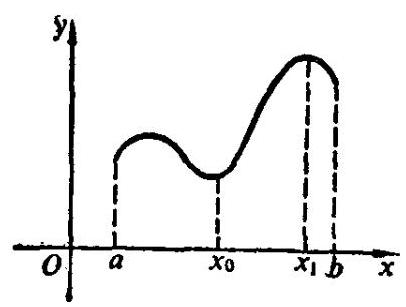
\includegraphics[max width=0.4\textwidth]{images/01912c18-5c3f-733d-b775-749ba9897a9d_34_898703.jpg}
\end{center}

图 1-8

性质 1 (最大值和最小值定理) 如果 \(f\left( x\right)\) 是闭区间 \(\left\lbrack {a,b}\right\rbrack\) 上的连续函数,那么 \(f\left( x\right)\) 在 \(\left\lbrack {a,b}\right\rbrack\) 上有最大值和最小值.

如图 1-8, \(f\left( {x}_{1}\right) \geq f\left( x\right) ,x \in \left\lbrack {a,b}\right\rbrack\) ;

\[
f\left( {x}_{0}\right) \leq f\left( x\right) ,\;x \in \left\lbrack {a,b}\right\rbrack .
\]

利用函数极限的运算法则, 还可以证明连续函数的和、 差、积、商仍然是连续函数.

性质 2 如果函数 \(f\left( x\right) \text{、}g\left( x\right)\) 在某一点 \(x = {x}_{0}\) 处连续, 那么

(1) \(f\left( x\right) \pm g\left( x\right)\) ,

(2) \(f\left( x\right) \cdot g\left( x\right)\) ,

(3) \(\frac{f\left( x\right) }{g\left( x\right) }\;\left( {g\left( x\right) \neq 0}\right)\)

在点 \(x = {x}_{0}\) 处都连续.

证明: 因为函数 \(f\left( x\right) \text{、}g\left( x\right)\) 在点 \(x = {x}_{0}\) 处连续,所以,

\[
\mathop{\lim }\limits_{{x \rightarrow {x}_{0}}}f\left( x\right) = f\left( {x}_{0}\right) ,\mathop{\lim }\limits_{{x \rightarrow {x}_{0}}}g\left( x\right) = g\left( {x}_{0}\right) .
\]

由极限的运算法则, 得出

\[
\mathop{\lim }\limits_{{x \rightarrow {x}_{0}}}\left\lbrack {f\left( x\right) \pm g\left( x\right) }\right\rbrack = \mathop{\lim }\limits_{{x \rightarrow {x}_{0}}}f\left( x\right) \pm \mathop{\lim }\limits_{{x \rightarrow {x}_{0}}}g\left( x\right)
\]

\[
= f\left( {x}_{0}\right) \pm g\left( {x}_{0}\right) \text{.}
\]

因此,函数 \(f\left( x\right) \pm g\left( x\right)\) 在点 \(x = {x}_{0}\) 处连续.

同样可以证明(2)和(3).

\begin{problemset}[练习]


\item 连续函数的图象有什么特点? 观察下列各函数图象, 说出函数在 \(x = a\) 处是否连续:

\begin{center}
	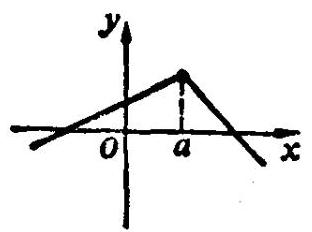
\includegraphics[max width=0.3\textwidth]{images/01912c18-5c3f-733d-b775-749ba9897a9d_35_115885.jpg}
	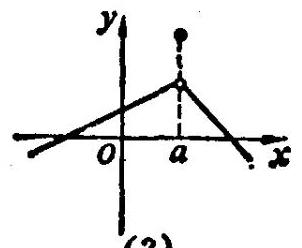
\includegraphics[max width=0.3\textwidth]{images/01912c18-5c3f-733d-b775-749ba9897a9d_35_560451.jpg}
	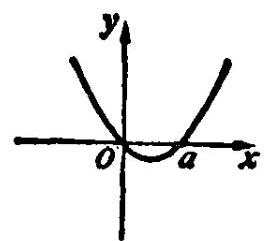
\includegraphics[max width=0.3\textwidth]{images/01912c18-5c3f-733d-b775-749ba9897a9d_35_351282.jpg}
\end{center}

\noindent % 确保表格从左边开始,不产生额外的缩进
\begin{tabular}{ccc}
	\makebox[0.3\textwidth][c]{(1)} &
	\makebox[0.3\textwidth][c]{(2)} &
	\makebox[0.3\textwidth][c]{(3)}
\end{tabular}

\begin{center}
	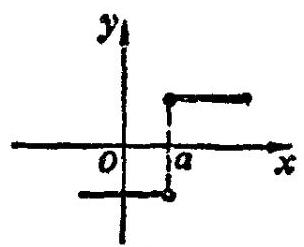
\includegraphics[max width=0.3\textwidth]{images/01912c18-5c3f-733d-b775-749ba9897a9d_36_706273.jpg}
	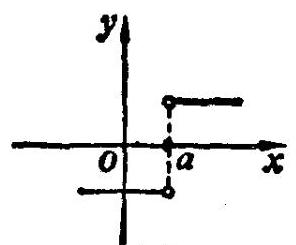
\includegraphics[max width=0.3\textwidth]{images/01912c18-5c3f-733d-b775-749ba9897a9d_36_222184.jpg}
	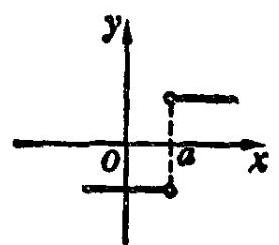
\includegraphics[max width=0.3\textwidth]{images/01912c18-5c3f-733d-b775-749ba9897a9d_36_774109.jpg}
\end{center}

\noindent % 确保表格从左边开始,不产生额外的缩进
\begin{tabular}{ccc}
	\makebox[0.3\textwidth][c]{(3)} &
	\makebox[0.3\textwidth][c]{(4)} &
	\makebox[0.3\textwidth][c]{(5)}
\end{tabular}

\begin{center}
	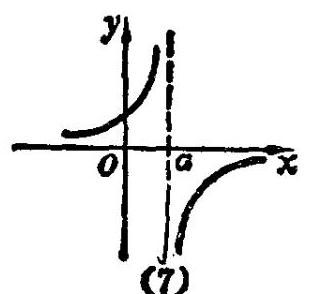
\includegraphics[max width=0.3\textwidth]{images/01912c18-5c3f-733d-b775-749ba9897a9d_36_255638.jpg}
	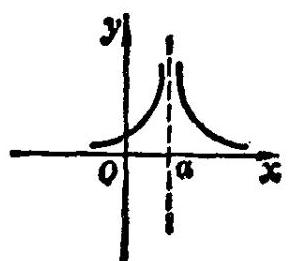
\includegraphics[max width=0.3\textwidth]{images/01912c18-5c3f-733d-b775-749ba9897a9d_36_333878.jpg}
	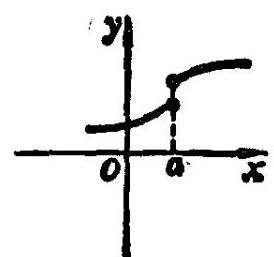
\includegraphics[max width=0.3\textwidth]{images/01912c18-5c3f-733d-b775-749ba9897a9d_36_561922.jpg}
\end{center}

\noindent % 确保表格从左边开始,不产生额外的缩进
\begin{tabular}{ccc}
	\makebox[0.3\textwidth][c]{(7)} &
	\makebox[0.3\textwidth][c]{(8)} &
	\makebox[0.3\textwidth][c]{(9)}
\end{tabular}


(第 1 题)

\item 结合下列函数的图象, 说明函数在给定点或区间上是否连续:

(1) \(f\left( x\right) = \frac{1}{{x}^{2}},x = 0\) ; (2) \(f\left( x\right) = \left| x\right| ,x = 0\) ;

(3) \(f\left( x\right) = \frac{{x}^{2} - 1}{x - 1},\left( {0,1}\right)\) ;

(4) \(f\left( x\right) = a{x}^{2} + {bx} + c,\left( {-\infty ,\infty }\right)\) .

\end{problemset}

\subsection*{复合函数的连续性}
我们学过的函数可以分为以下五类: .

幂函数 \(y = {x}^{\alpha }\) ( \(\alpha\) 是实数); 0.5

指数函数 \(y = {a}^{x}\left( {a > 0\text{,且}a \neq 1}\right)\) ;

对数函数 \(y = {\log }_{a}x\left( {a > 0\text{,且}a \neq 1}\right)\) ;

三角函数 \(y = \sin x,y = \cos x,y = \operatorname{tg}x,y = \operatorname{ctg}x\) ,等等;

反三角函数 \(y = \arcsin x,y = \arccos x,y = \operatorname{arctg}x\) ,

\(y = \operatorname{arcctg}x\) ,等等. 这五种函数统称基本初等函数.

关于基本初等函数的连续性有如下结论:

基本初等函数在其定义区间上是连续函数.

例如, \(y = {x}^{\frac{1}{2}}\) 在 \(\lbrack 0, + \infty )\) 上连续, \(y = \sin x\) 在 \(\left( {-\infty , + \infty }\right)\) 上连续, \(y = \operatorname{tg}x\) 在 \(\left( {{n\pi } - \frac{\pi }{2},{n\pi } + \frac{\pi }{2}}\right)\) 上连续.

我们以前学过的许多函数是由基本初等函数和常数经过有限次四则运算得出的. 例如, 二次函数

\[
y = a{x}^{2} + {bx} + c
\]

可以看作是由常数 \(a\) 乘以幂函数 \({x}^{2}\) 的积,加上常数 \(b\) 乘以幂函数 \(x\) 的积,再加上常数 \(c\) 而得到的一个函数.

另外还有一些函数,例如 \(y = \sin {2x}\) ,它和 \(y = \sin x\) 不同, 不是基本初等函数. 下面我们将会看到, 它是由三角函数 \(y = \sin u\) 和一次函数 \(u = {2x}\) 经过 “复合”而成的.

同样, 函数

\[
y = \sqrt{1 + {x}^{2}}
\]

是由幂函数 \(y = {u}^{\frac{1}{2}}\) 和二次函数 \(u = 1 + {x}^{2}\) 经过 “复合”而成的.

一般地说,如果 \(y\) 是 \(u\) 的函数,而 \(u\) 又是 \(x\) 的函数,即 \(y = f\left( u\right) ,u = g\left( x\right)\) ,那么 \(y\) 关于 \(x\) 的函数

\[
y = f\left\lbrack {g\left( x\right) }\right\rbrack
\]

叫做函数 \(f\) 和 \(g\) 的复合函数, \(u\) 叫做中间变量.

例 1 (1) 函数 \(y = f\left( u\right) = \lg u\) 与 \(u = g\left( x\right) = \sin x\) 经过 “复合”以后得到什么函数?

(2)函数 \(y = f\left( u\right) = \sin u\) 与 \(u = g\left( x\right) = \lg x\) 呢?

解: (1) \(\lg \sin x\) ;

(2) \(\sin \left( {\lg x}\right)\) .

复合函数也可以是由三个或三个以上的函数复合而成的.

例 2 说出下列函数是由哪几个简单的函数复合而成的:

(1) \(y = a\sin \left( {{bt} + c}\right)\) ;

(2) \(y = {\log }_{a}{\left( 1 + x\right) }^{2}\) .

解: (1) \(y = a\sin \left( {{bt} + c}\right)\) 可以看成是 \(y = a\sin u\) 和 \(u =\) \({bt} + c\) 两个函数复合而成的.

(2) \(y = {\log }_{a}{\left( 1 + x\right) }^{2}\) 可以看成是由 \(y = {\log }_{a}u,u = {v}^{2},v =\) \(1 + x\) 三个函数复合而成的.

一般地, 关于复合函数连续性有如下结论:

如果函数 \(u = g\left( x\right)\) 在点 \(x = {x}_{0}\) 处连续, \(g\left( {x}_{0}\right) = {u}_{0}\) ,且函数 \(y = f\left( u\right)\) 在点 \(u = {u}_{0}\) 处连续,那么复合函数 \(y = f\left\lbrack {g\left( x\right) }\right\rbrack\) 在点 \({x}_{0}\) 处连续.

由基本初等函数和常数经过有限次四则运算和有限次函数的复合而得出的函数, 统称初等函数.

由基本初等函数的连续性、连续函数的性质 2 和复合函数的连续性可以得出如下结论:

一切初等函数在它们的定义区间上是连续函数.

根据这条结论, 函数

\[
y = \frac{{ax} + b}{c{x}^{2} + d},\;y = a\sin \left( {{\omega t} + \varphi }\right) ,
\]

\[
y = {\log }_{a}{\left( 1 + x\right) }^{2},\;y = \sqrt{{a}^{2} - {b}^{2}{\cos }^{2}x},\;y = \frac{{e}^{x} - {e}^{-x}}{2}
\]

都是在其定义区间上的连续函数.

这个结论不仅给我们提供了判断一个函数是不是连续函数的根据, 而且为我们提供了计算初等函数的极限问题的一种方法. 这种方法是: 如果函数 \(f\left( x\right)\) 是初等函数,而且点 \({x}_{0}\) 是函数定义区间内的一点,那么求 \(x \rightarrow {x}_{0}\) 时函数 \(f\left( x\right)\) 的极限,只要求出 \(f\left( x\right)\) 在点 \({x}_{0}\) 处的函数值 \(f\left( {x}_{0}\right)\) 就可以了.

例 3 利用初等函数的连续性, 求下列极限:

(1) \(\mathop{\lim }\limits_{{x \rightarrow 1}}\sqrt{3 + {x}^{2}}\) ; (2) \(\mathop{\lim }\limits_{{x \rightarrow 0}}\frac{1 - {e}^{x}}{1 + {e}^{x}}\)

(3) \(\mathop{\lim }\limits_{{x \rightarrow \frac{\pi }{2}}}\ln \sin x\) ;

(4) \(\mathop{\lim }\limits_{{x \rightarrow a}}\sqrt{1 + {\operatorname{arctg}}^{2}\frac{x}{a}}\;\left( {a \neq 0}\right)\) .

解: (1) \(\mathop{\lim }\limits_{{x \rightarrow 1}}\sqrt{3 + {x}^{2}} = \sqrt{3 + {1}^{2}} = 2\) ;

(2) \(\mathop{\lim }\limits_{{x \rightarrow 0}}\frac{1 - {e}^{x}}{1 + {e}^{x}} = \frac{1 - {e}^{0}}{1 + {e}^{0}} = \frac{1 - 1}{1 + 1} = 0\) ;

(3) \(\mathop{\lim }\limits_{{x \rightarrow \frac{\pi }{2}}}\ln \sin x = \ln \sin \frac{\pi }{2} = \ln 1 = 0\) ;

(4) \(\mathop{\lim }\limits_{{x \rightarrow a}}\sqrt{1 + \operatorname{arctg}{}^{2}\frac{x}{a}} = \sqrt{1 + \operatorname{arctg}{}^{2}\frac{a}{a}}\)

\[
= \sqrt{1 + {\left( \frac{\pi }{4}\right) }^{2}}
\]

\[
= \frac{1}{4}\sqrt{{16} + {\pi }^{2}}
\]

例 4 求下列极限:

(1) \(\mathop{\lim }\limits_{{x \rightarrow 1}}\frac{\left( {x - 1}\right) \sqrt{2 - x}}{{x}^{4} - 1}\) ; (2) \(\mathop{\lim }\limits_{{x \rightarrow 0}}\frac{\sqrt{1 + x} - 1}{x}\) .

解: (1) \(\mathop{\lim }\limits_{{x \rightarrow 1}}\frac{\left( {x - 1}\right) \sqrt{2 - x}}{{x}^{4} - 1} = \mathop{\lim }\limits_{{x \rightarrow 1}}\frac{\sqrt{2 - x}}{{x}^{3} + {x}^{2} + x + 1}\)

\[
= \frac{\sqrt{2 - 1}}{{1}^{3} + {1}^{2} + 1 + 1}
\]

\[
= \frac{1}{4}\text{. }
\]

(2) \(\mathop{\lim }\limits_{{x \rightarrow 0}}\frac{\sqrt{1 + x} - 1}{x} = \mathop{\lim }\limits_{{x \rightarrow 0}}\frac{\left( {\sqrt{1 + x} - 1}\right) \left( {\sqrt{1 + x} + 1}\right) }{x\left( {\sqrt{1 + x} + 1}\right) }\)

\[
= \mathop{\lim }\limits_{{x \rightarrow 0}}\frac{x}{x\left( {\sqrt{1 + x} + 1}\right) }
\]

\[
= \mathop{\lim }\limits_{{x \rightarrow 0}}\frac{1}{\sqrt{1 + x} + 1} = \frac{1}{2}\text{. }
\]

\begin{problemset}[练习]

\item 下列函数是由基本初等函数经过哪些运算得出的函数?

(1) \(y = {ax} + b\) ; (2) \(y = \frac{1 + {x}^{2}}{ax}\) ;

(3) \(y = 5{a}^{x}\sin x\) ; (4) \(y = \left( {1 + \ln x}\right) \sin x\) .

\item 写出下列函数经过复合而成的函数的表示式:

(1) \(y = {e}^{u},u = {x}^{2}\) ; (2) \(y = {u}^{2},u = {e}^{x}\) ;

(3) \(y = \sqrt{u},u = 1 + {\sin }^{2}x\) ;

(4) \(y = a{u}^{2},u = \sin v,v = {bx} + c\) .

\item 说出下列函数是由哪几个简单的函数复合而成的:

(1) \(y = \sqrt{1 + {a}^{x}}\) ; (2) \(y = \ln {ax}\) ;

(3) \(y = \frac{1}{\cos \left( {1 + {x}^{2}}\right) }\) ; (4) \(y = \sqrt{{a}^{2} - {b}^{2}{\cos }^{2}x}\) .

\item 求下列极限:

(1) \(\mathop{\lim }\limits_{{x \rightarrow 0}}\lg \cos {3x}\) ; (2) \(\mathop{\lim }\limits_{{x \rightarrow \frac{\pi }{2}}}\frac{\sin {2x}}{\cos x}\)

(3) \(\mathop{\lim }\limits_{{x \rightarrow 1}}\frac{\sqrt{3 + {x}^{2}} - \sqrt{{x}^{2} - 1}}{x + 1}\)

(4) \(\mathop{\lim }\limits_{{x \rightarrow 0}}\frac{\left( {1 + {a}^{x}}\right) \left( {1 - \cos x}\right) }{{\sin }^{2}\frac{x}{2}}\) .

\end{problemset}
\section{两个重要的极限}

现在我们来讨论微积分中常常用到的两个重要的极限.

\subsection*{1. \(\mathop{\lim }\limits_{{x \rightarrow 0}}\frac{\sin x}{x} = 1\)}

为了证明这个极限, 我们先介绍一个有关极限的定理 (证明略).

定理 如果函数 \(f\left( x\right) ,g\left( x\right) ,h\left( x\right)\) 在点 \({x}_{0}\) 的附近满足:

(1) \(g\left( x\right) \leq f\left( x\right) \leq h\left( x\right)\) ,

(2) \(\mathop{\lim }\limits_{{x \rightarrow {x}_{0}}}g\left( x\right) = A,\mathop{\lim }\limits_{{x \rightarrow {x}_{0}}}h\left( x\right) = A\) ( \(A\) 是常数),

那么有

\[
\mathop{\lim }\limits_{{x \rightarrow {x}_{0}}}f\left( x\right) = A\text{. }
\]

现在我们来讨论 \(\mathop{\lim }\limits_{{x \rightarrow 0}}\frac{\sin x}{x}\) . 为此,我们先列出当 \(x\) 接近于 0 时函数 \(\frac{\sin x}{x}\) 的值如下表,并作出函数的图象 (图 1-9).

\begin{center}
	\adjustbox{max width=\textwidth}{
		\begin{tabular}{|c|c|c|}
			\hline
			\(x\) (弧度) & \(\sin x\) & \(\frac{\sin x}{x}\) \\
			\hline
			1.000 & 0.84147098 & 0.84147098 \\
			\hline
			0.100 & 0.099833417 & 0.99833417 \\
			\hline
			0.010 & 0.0099998334 & 0.99998334 \\
			\hline
			0.001 & 0.00099999984 & 0.99999984 \\
			\hline
		\end{tabular}
	}
\end{center}

\begin{center}
	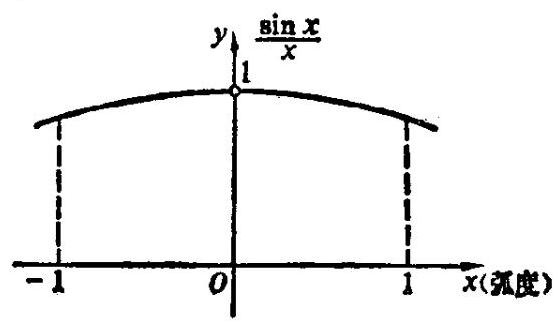
\includegraphics[max width=0.6\textwidth]{images/01912c18-5c3f-733d-b775-749ba9897a9d_42_483969.jpg}
\end{center}

图 1-9

\begin{center}
	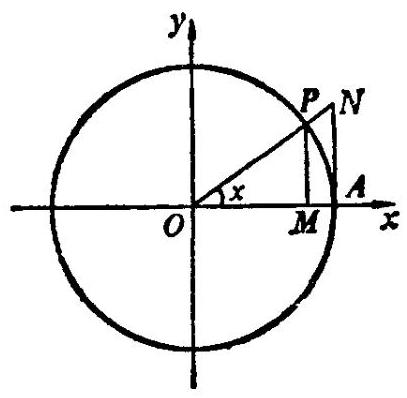
\includegraphics[max width=0.4\textwidth]{images/01912c18-5c3f-733d-b775-749ba9897a9d_42_838953.jpg}
\end{center}

图 1-10

从上表和图 1-9 可以看出,当 \(x\) 无限趋近于 0 时,函数 \(\frac{\sin x}{x}\) 的值无限趋近于 1,即 \(\mathop{\lim }\limits_{{x \rightarrow 0}}\frac{\sin x}{x} = 1\) . 下面我们利用上面的定理来证明这个结论.

如图 1-10,在单位圆中,以 \({OA}\) 为始边的圆心角 \(x\) (不大的正角) 是用弧度来度量的,角的终边与圆相交于 \(P.{MP} \bot\) \({OA},{AN}\) 是过圆 \(O\) 上 \(A\) 点的切线,它和 \({OP}\) 相交于 \(N\) . 从图中知道,

\[
{MP} = \sin x,\overset{⏜}{PA} = x,{AN} = \operatorname{tg}x,
\]

那么面积

\[
{S}_{\bigtriangleup {OAP}} = \frac{1}{2}\sin x,{S}_{\text{焦形 }{OAP}} = \frac{1}{2}x,
\]

\[
{S}_{\bigtriangleup {OAN}} = \frac{1}{2}\operatorname{tg}x.
\]

由

\[
{S}_{\bigtriangleup {OAP}} < {S}_{\text{底形 }{OAP}} < {S}_{\bigtriangleup {OAN}},
\]

得

\[
\sin x < x < \operatorname{tg}x\text{.}
\]

当自变量 \(x\) 取正值趋近于 0 时, \(\sin x > 0\) ,因此,

\[
1 < \frac{x}{\sin x} < \frac{\operatorname{tg}x}{\sin x}
\]

即

\[
1 < \frac{x}{\sin x} < \frac{1}{\cos x}
\]

于是,

\[
\cos x < \frac{\sin x}{x} < 1\text{.}
\]

因为余弦函数是连续函数,所以 \(\mathop{\lim }\limits_{{x \rightarrow 0 + }}\cos x = 1\) . 根据上面判定函数极限存在的定理,得到当 \(x\) 取正值趋近于 0 时,

\[
\mathop{\lim }\limits_{{x \rightarrow 0 + }}\frac{\sin x}{x} = 1
\]

又当 \(x\) 取负值趋近于 0 时, \(- x \rightarrow 0, - x > 0,\sin \left( {-x}\right)\) \(> 0\) ,于是

\[
\mathop{\lim }\limits_{{x \rightarrow 0 - }}\frac{\sin x}{x} = \mathop{\lim }\limits_{{-x \rightarrow 0 + }}\frac{\sin \left( {-x}\right) }{-x} = 1.
\]

根据 1.3 节最后的定理, 由于

\[
\mathop{\lim }\limits_{{x \rightarrow 0 + }}\frac{\sin x}{x} = \mathop{\lim }\limits_{{x \rightarrow 0 - }}\frac{\sin x}{x} = 1
\]

所以有

\[
\mathop{\lim }\limits_{{x \rightarrow 0}}\frac{\sin x}{x} = 1
\]

在推导这个重要极限时,用到 \({S}_{\text{扇形 }{OAP}} = \frac{1}{2}x,x\) 以弧度为单位. 一般地, 在微积分中三角函数的自变量都是实数, 它对应于以弧度为单位的角或弧.

例 1 求 \(\mathop{\lim }\limits_{{x \rightarrow 0}}\frac{\operatorname{tg}x}{x}\) .

解: \(\mathop{\lim }\limits_{{x \rightarrow 0}}\frac{\operatorname{tg}x}{x} = \mathop{\lim }\limits_{{x \rightarrow 0}}\left( {\frac{\sin x}{x} \cdot \frac{1}{\cos x}}\right)\)

\[
= \mathop{\lim }\limits_{{x \rightarrow 0}}\frac{\sin x}{x} \cdot \mathop{\lim }\limits_{{x \rightarrow 0}}\frac{1}{\cos x}
\]

\[
= 1 \times 1 = 1\text{.}
\]

例 2 求 \(\mathop{\lim }\limits_{{x \rightarrow 0}}\frac{1 - \cos x}{{x}^{2}}\) .

解: \(\mathop{\lim }\limits_{{x \rightarrow 0}}\frac{1 - \cos x}{{x}^{2}} = \mathop{\lim }\limits_{{x \rightarrow 0}}\frac{2{\sin }^{2}\frac{x}{2}}{{x}^{2}}\)

\[
= \frac{1}{2}\mathop{\lim }\limits_{{x \rightarrow 0}}\frac{{\sin }^{2}\frac{x}{2}}{{\left( \frac{x}{2}\right) }^{2}}
\]

\(= \frac{1}{2}\mathop{\lim }\limits_{{\frac{x}{2} \rightarrow 0}}{\left( \frac{\sin \frac{x}{2}}{\frac{x}{2}}\right) }^{2}\left( {\text{ 当 }x \rightarrow 0\text{ 时,}\;\frac{x}{2} \rightarrow 0}\right)\)

\[
= \frac{1}{2}\mathop{\lim }\limits_{{\frac{x}{2} \rightarrow 0}}\left( \frac{\sin \frac{x}{2}}{\frac{x}{2}}\right) \cdot \mathop{\lim }\limits_{{\frac{x}{2} \rightarrow 0}}\left( \frac{\sin \frac{x}{2}}{\frac{x}{2}}\right) = \frac{1}{2} \times 1 \times 1 = \frac{1}{2}\text{.}
\]

\subsection*{2. \(\mathop{\lim }\limits_{{x \rightarrow \infty }}{\left( 1 + \frac{1}{x}\right) }^{x} = e\)}

我们从下表可以看出当 \(x \rightarrow + \infty\) 时函数 \({\left( 1 + \frac{1}{x}\right) }^{x}\) 的变化趋势:

\begin{center}
	\adjustbox{max width=\textwidth}{
		\begin{tabular}{|c|c|c|}
			\hline
			\(x\) & \({\left( 1 + \frac{1}{x}\right) }^{x}\) & 近 似 值 \\
			\hline
			1 & \({\left( 1 + \frac{1}{1}\right) }^{1}\) & 2 \\
			\hline
			10 & \({\left( 1 + \frac{1}{10}\right) }^{10}\) & 2. 59374 \\
			\hline
			100 & \({\left( 1 + \frac{1}{100}\right) }^{100}\) & 2. 70481 \\
			\hline
			1000 & \({\left( 1 + \frac{1}{1000}\right) }^{1000}\) & 2. 71692 \\
			\hline
			10000 & \({\left( 1 + \frac{1}{10000}\right) }^{10000}\) & 2. 71815 \\
			\hline
			100000 & \({\left( 1 + \frac{1}{100000}\right) }^{100000}\) & 2. 71827 \\
			\hline
			\(\cdots\) & \(\cdots\) & \(\cdots\) \\
			\hline
		\end{tabular}
	}
\end{center}

同样,当 \(x \rightarrow - \infty\) 时,函数 \({\left( 1 + \frac{1}{x}\right) }^{x}\) 有相同的变化趋势 (见下页的表).

可以证明,当 \(x\) 趋向无穷时, \({\left( 1 + \frac{1}{x}\right) }^{x}\) 趋近于无理数 \({2.71828182845}\cdots\) ,记作 \(e\) . 即

\[
\mathop{\lim }\limits_{{x \rightarrow \infty }}{\left( 1 + \frac{1}{x}\right) }^{x} = e
\]

\begin{center}
	\adjustbox{max width=\textwidth}{
		\begin{tabular}{|c|c|c|}
			\hline
			\(- 2\) & \({\left( 1 + \frac{1}{-2}\right) }^{-2}\) & 4 \\
			\hline
			\(- {10}\) & \({\left( 1 + \frac{1}{-{10}}\right) }^{-{10}}\) & 2. 86797 \\
			\hline
			\(- {100}\) & \({\left( 1 + \frac{1}{-{100}}\right) }^{-{100}}\) & 2. 73199 \\
			\hline
			\(- {1000}\) & \({\left( 1 + \frac{1}{-{1000}}\right) }^{-{1000}}\) & 2. 71964 \\
			\hline
			\(- {10000}\) & \({\left( 1 + \frac{1}{-{10000}}\right) }^{-{10000}}\) & 2. 71842 \\
			\hline
			\(- {100000}\) & \({\left( 1 + \frac{1}{-{100000}}\right) }^{-{100000}}\) & 2. 71830 \\
			\hline
			\(\cdots\) & \(\cdots\) & \(\cdots\) \\
			\hline
		\end{tabular}
	}
\end{center}

如果作一个变换 \(y = \frac{1}{x}\) ,那么当 \(x \rightarrow \infty\) 时, \(y \rightarrow 0\) ,于是又得到

\[
\mathop{\lim }\limits_{{y \rightarrow 0}}{\left( 1 + y\right) }^{\frac{1}{y}} = e
\]

无理数 \(e\) 是自然对数的底,它在微积分和其他科学技术中经常用到.

例 3 求 \(\mathop{\lim }\limits_{{x \rightarrow \infty }}{\left( 1 + \frac{1}{x}\right) }^{-x}\) .

解: \(\mathop{\lim }\limits_{{x \rightarrow \infty }}{\left( 1 + \frac{1}{x}\right) }^{-x} = \mathop{\lim }\limits_{{x \rightarrow \infty }}\frac{1}{{\left( 1 + \frac{1}{x}\right) }^{x}}\)

\[
= \frac{1}{\mathop{\lim }\limits_{{x \rightarrow \infty }}{\left( 1 + \frac{1}{x}\right) }^{x}} = \frac{1}{e}
\]

\begin{problemset}[练习]

\item 求下列极限:

(1) \(\mathop{\lim }\limits_{{x \rightarrow 0}}\frac{x}{\sin x}\) 

(2) \(\mathop{\lim }\limits_{{x \rightarrow 0}}\frac{\sin {4x}}{3x}\) .

\item 求下列极限:

(1) \(\mathop{\lim }\limits_{{x \rightarrow \infty }}{\left( 1 + \frac{1}{x}\right) }^{2x}\)

(2) \(\mathop{\lim }\limits_{{x \rightarrow 0}}{\left( 1 + x\right) }^{-\frac{1}{x}}\) .
\end{problemset}

\begin{problemset}[习 题 三]


\item 根据函数连续性的定义, 说明下列函数在给定点处连续:

(1) \(f\left( x\right) = {3x} + 1,x = \frac{1}{2}\) ;

(2) \(f\left( x\right) = a{x}^{2} + b,x = 1\) ;

(3) \(f\left( x\right) = \frac{4{x}^{2} - 1}{{2x} - 1},x = 2\) ;

(4) \(f\left( x\right) = a{x}^{3} + b{x}^{2} + {cx} + d,x = 0\) .

\item 说出下列函数在实数轴上哪些点处不连续:

(1) \(y = \frac{1}{{x}^{2} + {3x} + 2}\) (2) \(y = \frac{1}{\sin x}\) .

\item 写出由下列各组函数复合而成的复合函数:

(1) \(y = {u}^{2},u = \sin x\) ;

(2) \(y = \sin u,u = {x}^{2}\) ;

(3) \(y = {u}^{3},u = {x}^{2} + 1\) ;

(4) \(y = \ln \dot{u};u = {v}^{2} + 1,v = \sin x\) ;

(5) \(y = {e}^{u},u = {v}^{2},v = \operatorname{ctg}x\) ;

(6) \(y = \arcsin u,u = \sqrt{v},v = \frac{x - a}{b - a}\) .

\item 下列函数是由哪几个简单函数复合而成的?

(1) \(y = {\left( 1 + x\right) }^{5}\) ; (2) \(y = \frac{1}{{\left( 1 - {x}^{2}\right) }^{3}}\) ;

(3) \(y = \ln {\sin }^{2}{3x}\) ; (4) \(y = {e}^{2{\cos }^{2}x}\) ;

(5) \(y = \frac{1}{\sqrt{1 - \operatorname{tg}{3x}}}\) ; (6) \(y = {\left( 1 + \operatorname{arctg}{x}^{2}\right) }^{8}\) .

\item 求下列极限:

(1) \(\mathop{\lim }\limits_{{x \rightarrow 1}}\sqrt{{x}^{2} + {3x} - 2}\) ; (2) \(\mathop{\lim }\limits_{{u \rightarrow 1}}\frac{{u}^{2} + u + 2}{3 - u}\) ;

(3) \(\mathop{\lim }\limits_{{x \rightarrow {16}}}\frac{\sqrt[4]{x} - 2}{\sqrt{x} - 4}\) (4) \(\mathop{\lim }\limits_{{x \rightarrow 2}}\frac{\sqrt{{2x} - 2} - \sqrt{x}}{{x}^{2} - 4}\) ;

(5) \(\mathop{\lim }\limits_{{\alpha \rightarrow \frac{\pi }{4}}}{\left( 1 + \sin 2\alpha \right) }^{2}\) ; (6) \(\mathop{\lim }\limits_{{x \rightarrow 2}}{\log }_{3}\left( {{x}^{3} + 1}\right)\) .

\item 求下列极限:

(1) \(\mathop{\lim }\limits_{{x \rightarrow 0}}\frac{x}{\operatorname{tg}{3x}}\) (2) \(\mathop{\lim }\limits_{{x \rightarrow 0}}\frac{\sin {3x}}{\sin {5x}}\)

(3) \(\mathop{\lim }\limits_{{x \rightarrow 0}}\frac{\sin x\operatorname{tg}x}{{x}^{2}}\) (4) \(\mathop{\lim }\limits_{{x \rightarrow 0}}\frac{1 - \cos {2x}}{x\sin x}\) .

\item 求下列极限:

(1) \(\mathop{\lim }\limits_{{x \rightarrow \infty }}{\left( 1 + \frac{1}{x}\right) }^{x + 2}\) (2) \(\mathop{\lim }\limits_{{x \rightarrow \infty }}{\left( 1 + \frac{2}{x}\right) }^{\frac{x}{2}}\)

(3) \(\mathop{\lim }\limits_{{x \rightarrow 0}}{\left( 1 + 2x\right) }^{\frac{1}{x}}\) (4) \(\mathop{\lim }\limits_{{x \rightarrow \infty }}{\left( 1 - \frac{1}{x}\right) }^{2x}\) .
\end{problemset}

\chapter*{小 结}
\markboth{小 结}{小 结}

一、本章的主要内容是数列的极限的概念及其运算法则; 函数的极限的概念及其运算法则; 函数连续的概念和初等函数的连续性; 两个重要的极限, 即

\[
\mathop{\lim }\limits_{{x \rightarrow 0}}\frac{\sin x}{x} = 1,\;\mathop{\lim }\limits_{{x \rightarrow \infty }}{\left( 1 + \frac{1}{x}\right) }^{x} = e.
\]

二、极限是描述数列和函数在无限过程中的变化趋势的重要概念. 极限方法是人们从有限中认识无限, 从近似中认识精确, 从量变中认识质变的一种数学方法, 它是微积分的基本思想和方法.

数列的极限与函数的极限的运算法则是类似的: 两个数列 (或函数) 的和、差、积、商的极限分别等于这两个数列 (或函数) 的极限的和、差、积、商 (作为除数的数列或函数的极限不能为零). 运用这些运算法则, 可以简化极限的计算过程.

三、连续的概念是用极限的概念定义的, 但是连续和极限是有区别的: 极限所讨论的是函数在某一点附近的变化趋势, 而不管函数在这一点上是否有定义或取什么值; 函数在一点处连续不仅要求在这一点有极限, 而且要求极限同这一点的函数值相等.

四、幂函数、指数函数、对数函数、三角函数和反三角函数, 统称基本初等函数.

由基本初等函数和常数经过有限次四则运算和有限次函数的复合而得出的函数, 统称初等函数.

基本初等函数和一切初等函数在它们的定义区间上是连续函数。

\chapter*{复习参考题一}
\markboth{复习参考题一}{复习参考题一}
\section*{\(A\) 组}

1. 求无穷等比数列 \(\left\{ {q}^{n}\right\}\) 当 \(q = \frac{1}{2}\) 时前 10 项的和与前 100 项的和。

2. 作图表示下列无穷数列, 并说出数列是否趋近于某一常数:

(1) \(\left\{ {1 + {\left( -1\right) }^{n}\frac{2}{n}}\right\}\) (2) \(\left\{ \frac{{\left( n - 1\right) }^{2}}{2n}\right\}\)

(3) \(\left\{ {\left( -\frac{1}{n}\right) }^{3}\right\}\) (4) \(\{ \sqrt{n}\}\) .

3. 已知数列 \(\left\{ \frac{1}{{3}^{n}}\right\}\) ,根据下表中给出的 \(\varepsilon\) 的数值,求出相应的正整数 \(N\) ,使得当 \(n > N\) 时, \(\left| {\frac{1}{{3}^{n}} - 0}\right| < \varepsilon\) 恒成立.

\begin{center}
	\adjustbox{max width=\textwidth}{
		\begin{tabular}{|c|c|c|c|c|}
			\hline
			e & 0.1 & 0.02 & 0.003 & 0.0001 \\
			\hline
			\(N\) & \phantom{X} & \phantom{X} & \phantom{X} & \phantom{X} \\
			\hline
		\end{tabular}
	}
\end{center}

4. 举出两个极限是 7 的无穷数列.

5. 举出两个没有极限的无穷数列。

6. 求下列数列的极限:

(1) \(\mathop{\lim }\limits_{{n \rightarrow \infty }}\frac{{2n} + 1}{n}\) (2) \(\mathop{\lim }\limits_{{n \rightarrow \infty }}\frac{3n}{n + 1}\)

(3) \(\mathop{\lim }\limits_{{n \rightarrow \infty }}\frac{{n}^{2}}{{n}^{2} - n}\) (4) \(\mathop{\lim }\limits_{{n \rightarrow \infty }}\frac{1}{{n}^{2} + 1}\) .

7. (1) 求 \(\mathop{\lim }\limits_{{n \rightarrow \infty }}\frac{1 + 2 + 3 + \cdots + n}{1 + 3 + 5 + \cdots + \left( {{2n} - 1}\right) }\) ;

(2)求 \(\mathop{\lim }\limits_{{n \rightarrow \infty }}\frac{1 + \frac{1}{2} + \frac{1}{4} + \cdots + \frac{1}{{2}^{n}}}{1 + \frac{1}{3} + \frac{1}{9} + \cdots + \frac{1}{{3}^{n}}}\) .

8. 求下列极限:

(1) \(\mathop{\lim }\limits_{{n \rightarrow \infty }}\left( {\frac{1}{n} + \frac{{2n} - 1}{3n}}\right)\) ; (2) \(\mathop{\lim }\limits_{{n \rightarrow \infty }}\frac{5{n}^{2} + 7}{3{n}^{2} + n - 1}\)

(3) \(\mathop{\lim }\limits_{{n \rightarrow \infty }}\frac{\left( {n - 1}\right) \left( {n + 1}\right) \left( {n + 2}\right) }{2{n}^{3}}\) ; (4) \(\mathop{\lim }\limits_{{n \rightarrow \infty }}\frac{{\left( n - 1\right) }^{3}}{{n}^{3} + 1}\) ;

(5) \(\mathop{\lim }\limits_{{x \rightarrow 1}}\left( {\frac{1}{1 - x} - \frac{3}{1 - {x}^{3}}}\right)\) ;

(6) \(\mathop{\lim }\limits_{{x \rightarrow \infty }}\left( {\frac{{x}^{3}}{2{x}^{2} - 1} - \frac{{x}^{2}}{{2x} + 1}}\right)\) .

9. 已知 \(f\left( x\right) = \frac{{a}_{0}{x}^{m} + {a}_{1}{x}^{m - 1} + \cdots + {a}_{m}}{{b}_{0}{x}^{m} + {b}_{1}{x}^{n - 1} + \cdots + {b}_{n}}\) ,而且 \({x}_{0}\) 不是 \(f\left( x\right)\) 的分母的根:

(1)求 \(\mathop{\lim }\limits_{{x \rightarrow {x}_{0}}}f\left( x\right)\) ;

(2)当 \(m \leq n\) 时,求 \(\mathop{\lim }\limits_{{x \rightarrow \infty }}f\left( x\right)\) .

10. 说出下列函数是怎样复合而成的:

(1) \(y = {\left( a + bx\right) }^{5}\) ; (2) \(y = {\left( \arccos \sqrt{1 - {x}^{2}}\right) }^{3}\) ;

(3) \(y = \operatorname{arctg}\sqrt[5]{{x}^{3} - 1}\) ; (4) \(y = {e}^{\frac{1}{2}\lg \left( {{ax} + b}\right) }\) .

11. 求下列极限:

(1) \(\mathop{\lim }\limits_{{x \rightarrow \sqrt{2}}}\frac{2{x}^{2} - 1}{{x}^{4} + 2{x}^{2} - 1}\) (2) \(\mathop{\lim }\limits_{{a \rightarrow \frac{\pi }{3}}}\left( {\sin {2\theta } + \cos {2\theta }}\right)\) ;

(3) \(\mathop{\lim }\limits_{{x \rightarrow a}}\frac{\sin x - \sin a}{x - a}\) ; (4) \(\mathop{\lim }\limits_{{x \rightarrow 0}}\frac{{\sin }^{2}{3x}}{x\sin {2x}}\)

(5) \(\mathop{\lim }\limits_{{x \rightarrow 2}}\frac{x - 2}{\sqrt{x - 1} - 1}\) ; (6) \(\mathop{\lim }\limits_{{x \rightarrow 3}}\frac{\sqrt{1 + x} - 2}{x - 3}\) .

12. 求下列极限:

(1) \(\mathop{\lim }\limits_{{x \rightarrow 0}}\frac{{x}^{2}}{{\sin }^{2}\left( \frac{x}{3}\right) }\) (2) \(\mathop{\lim }\limits_{{x \rightarrow 0}}\left( {x \cdot \operatorname{ctg}x}\right)\) ;

(3) \(\mathop{\lim }\limits_{{x \rightarrow \infty }}{\left( \frac{x}{1 + x}\right) }^{x}\) ; (4) \(\mathop{\lim }\limits_{{x \rightarrow \infty }}{\left( 1 + \frac{2}{x}\right) }^{x}\) .

\section*{B 组}

13. 下面的数列中, 哪些有极限? 如果数列有极限, 说出它的极限。

(1) \(1,{0.1},{0.01},{0.001},\cdots \cdots\) ;

(2) \(+ 2, - 2, + 2, - 2,\cdots \cdots\) ;

(3) \(\left\{ \frac{\sqrt{n} + 1}{n}\right\}\)

(4) \(\left\{ {q}^{n}\right\}\) (提示: 分 \(q = 1,q = - 1;\left| q\right| < 1,\left| q\right| > 1\) 四种情况讨论).

14. 已知 \(a > 0\) ,求下列极限:

(1) \(\mathop{\lim }\limits_{{n \rightarrow \infty }}\frac{1}{1 + {a}^{n}}\) (2) \(\mathop{\lim }\limits_{{n \rightarrow \infty }}\frac{{a}^{n}}{1 + {a}^{n}}\) .

15. 如图,从 \(\angle {BAC}\) 的边上一点 \(B\) 作 \({BC} \bot {AC}\) ,从 \(C\) 作 \({CD} \bot\) \({AB}\) ,从 \(D\) 再作 \({DE} \bot {AC}\) ,这样无限进行下去. 假定 \({BC} =\) \(7\mathrm{\;{cm}},{CD} = 6\mathrm{\;{cm}}\) ,求这些垂线长的和.

\begin{center}
	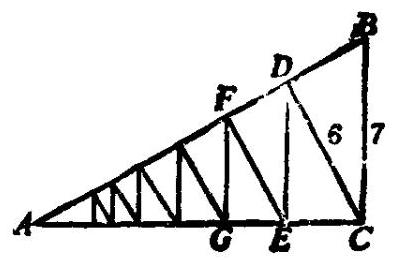
\includegraphics[max width=0.4\textwidth]{images/01912c18-5c3f-733d-b775-749ba9897a9d_52_461588.jpg}
\end{center}

(第 15 题)

16. 将下列循环小数化成分数:

(1) \({0.2}\dot{7}\) ; (2) 2.5142857 .

17. 求下列极限:

(1) \(\mathop{\lim }\limits_{{x \rightarrow \infty }}\frac{{x}^{2} + 2}{{x}^{2} + x + 1}\)

(2) \(\mathop{\lim }\limits_{{x \rightarrow \infty }}\frac{{x}^{2} + 1}{4{x}^{3} - 1}\)

(3) \(\mathop{\lim }\limits_{{x \rightarrow - \infty }}\frac{3{x}^{2} - 1}{{x}^{2} + {2x}}\)

(4) \(\mathop{\lim }\limits_{{x \rightarrow + \infty }}\frac{5{x}^{2} + x - 3}{4{x}^{2} - {2x} + 1}\) .

18. 求下列极限:

(1) \(\mathop{\lim }\limits_{{x \rightarrow 3}}\frac{{x}^{2} - 9}{{x}^{2} - {4x} + 3}\) (2) \(\mathop{\lim }\limits_{{u \rightarrow 1}}\frac{{u}^{3} - 1}{{u}^{2} - 1}\)

(3) \(\mathop{\lim }\limits_{{x \rightarrow 1}}\frac{{x}^{m} - 1}{{x}^{n} - 1}\;\left( {m,n\text{是自然数}}\right)\) .

19. 求下列无穷数列各项的和 \(S\) :

(1) \(\frac{1}{1 \cdot 2},\frac{1}{2 \cdot 3},\cdots ,\frac{1}{n\left( {n + 1}\right) },\cdots\)

\[
\text{提示:}\left. {\frac{1}{n\left( {n + 1}\right) } = \frac{1}{n} - \frac{1}{n + 1}}\right\rbrack \text{;}
\]

(2) \(\frac{2}{{2}^{2} - 1},\frac{2}{{3}^{2} - 1},\cdots ,\frac{2}{{\left( n + 1\right) }^{2} - 1},\cdots\)

\[
\left\lbrack {\text{提示:}\frac{1}{{\left( n + 1\right) }^{2} - 1} = \frac{1}{n\left( {n + 2}\right) }}\right\rbrack \text{.}
\]

20. 求下列极限:

(1) \(\mathop{\lim }\limits_{{x \rightarrow 1}}\frac{\sqrt[3]{x} - 1}{\sqrt{x} - 1}\)

(2) \(\mathop{\lim }\limits_{{x \rightarrow \infty }}\left( {\sqrt{{x}^{2} + 1} - \sqrt{{x}^{2} - 1}}\right)\) .

21. 求下列极限:

(1) \(\mathop{\lim }\limits_{{x \rightarrow \infty }}{\left( 1 + \frac{3}{x}\right) }^{x}\) ; (2) \(\mathop{\lim }\limits_{{x \rightarrow 0}}{\left( 1 + x\right) }^{\frac{1}{x} + 2}\) ;

(3) \(\mathop{\lim }\limits_{{x \rightarrow 0}}{\left( 1 + \operatorname{tg}x\right) }^{\operatorname{ctg}x}\) ; (4) \(\mathop{\lim }\limits_{{x \rightarrow 1}}\frac{\sin \left( {1 - x}\right) }{1 - {x}^{2}}\) .

\chapter{导数和微分}

\section*{导 数 概 念}

\section{瞬时速度}

我们知道,物体作匀速直线运动时,物体的位移 \(s\) 与所经过的时间 \(t\) 的比,就是物体运动的速度 \(v\) ,即

\[
v = \frac{s}{t}
\]

这个速度在匀速直线运动过程中的任何时刻都是一样的.

如果物体作非匀速直线运动, 也就是说, 在运动过程的各个时刻, 物体运动的快慢不一样, 这时, 设已知物体的运动规律是 \(s = s\left( t\right)\) ,从 \({t}_{0}\) 到 \({t}_{0} + {\Delta t}({\Delta t}\) 称为时间改变量) 这段时间内, 物体的位移 (即位置改变量) 是

\[
{\Delta s} = s\left( {{t}_{0} + {\Delta t}}\right) - s\left( {t}_{0}\right) ,
\]

那么,位置改变量 \({\Delta s}\) 与时间改变量 \({\Delta t}\) 的比,就是这段时间内物体的平均速度 \(\bar{v}\) ,即

\[
\bar{v} = \frac{\Delta s}{\Delta t} = \frac{s\left( {{t}_{0} + {\Delta t}}\right) - s\left( {t}_{0}\right) }{\Delta t}.
\]

平均速度的大小反映在这段时间内物体运动快慢的平均程度.

为了更精确地刻划非匀速运动, 还需知道物体在某一时刻的“速度”. 那么, 作非匀速直线运动的物体在某一时刻的 “速度”怎样求呢?

现在我们以自由落体运动为例, 来说明作非匀速直线运动的物体在某一时刻的“速度”的求法.

我们知道, 自由落体运动的方程是

\[
s = s\left( t\right) = \frac{1}{2}g{t}^{2},
\]

这里 \(g\) 是重力加速度,通常取 \(g = {9.8}\) 米 \(/{\text{秒}}^{2}\) . 现在来求 \(t = 3\) 秒这一时刻落体的 “速度”.

当 \({\Delta t}\) 很小时,从 3 秒到 \(3 + {\Delta t}\) 秒这段时间内,落体运动的快慢变化也不大, 因此, 可以用这段时间内的平均速度近似地反映落体在 3 秒时的 “速度”. 当 \({\Delta t}\) 越小时,一般来讲,这种近似就越精确. 现在我们来计算一下 \(t\) 从 3 秒 分别到 3.1 秒、 3.01 秒、 3.001 秒、 3.0001 秒、……, 各段时间内的平均速度, 把所得数据列表如下:

\begin{center}
\adjustbox{max width=\textwidth}{
\begin{tabular}{|c|c|c|c|c|}
\hline
\(t\left( \text{ 秒 }\right)\) & 8 (米) & \({\Delta t}\) (秒) & \({\Delta s}\) (米) & \(\bar{v} = \frac{\Delta s}{\Delta t}\left( {\text{ 米 }/\text{ 秒 }}\right)\) \\
\hline
3 & 4. \(5\mathrm{\;g}\) & \phantom{X} & \phantom{X} & \phantom{X} \\
\hline
3. 1 & \({4.805g}\) & 0.1 & \({0.305g}\) & \({3.05g}\) \\
\hline
3.01 & 4. \({53005g}\) & 0.01 & 0.03005g & 3. \({005}\mathrm{\;g}\) \\
\hline
3.001 & 4. 5030005g & 0.001 & 0.0030005g & 3.00059 \\
\hline
3.0001 & 4.500300005g & 0.0001 & 0.000300005g & 3.00005g \\
\hline
\(\cdots\) & ... & . & ... & ... \\
\hline
\end{tabular}
}
\end{center}

从上表可以看出,平均速度 \(\frac{\Delta s}{\Delta t}\) 随着 \({\Delta t}\) 变化而变化,当

\({\Delta t}\) 越小时, \(\frac{\Delta s}{\Delta t}\) 越接近于一个定值一 \({3g}\) . 这个值就是 \({\Delta t} \rightarrow 0\) 时 \(\frac{\Delta s}{\Delta t}\) 的极限. 我们规定这个极限为落体在 \(t = 3\) 秒时的速度,也叫瞬时速度,用 \(v\) 表示. 根据第一章求极限的法则,得

\[
v = \mathop{\lim }\limits_{{{\Delta t} \rightarrow 0}}\frac{s\left( {3 + {\Delta t}}\right) - s\left( 3\right) }{\Delta t}
\]

\[
= \mathop{\lim }\limits_{{{\Delta t} \rightarrow 0}}\frac{\frac{1}{2}g{\left( 3 + \Delta t\right) }^{2} - \frac{1}{2}g \cdot {3}^{2}}{\Delta t}
\]

\[
= \frac{g}{2}\mathop{\lim }\limits_{{{\Delta t} \rightarrow 0}}\left( {6 + {\Delta t}}\right)
\]

\[
= {3g} = {29.4}\text{ (米/秒). }
\]

一般地,我们规定,非匀速直线运动在某一时刻 \({t}_{0}\) 的瞬时速度 \(v\) ,就是运动物体在 \({t}_{0}\) 到 \({t}_{0} + {\Delta t}\) 一段时间内的平均速度当 \({\Delta t} \rightarrow 0\) 时的极限,即

\[
v = \mathop{\lim }\limits_{{{\Delta t} \rightarrow 0}}\frac{\Delta s}{\Delta t} = \mathop{\lim }\limits_{{{\Delta t} \rightarrow 0}}\frac{s\left( {{t}_{0} + {\Delta t}}\right) - s\left( {t}_{0}\right) }{\Delta t}.
\]

平均速度 \(\frac{\Delta s}{\Delta t}\) 在 \({\Delta t} \rightarrow 0\) 时转化为瞬时速度,瞬时速度的大小刻划了物体在某一时刻运动的快慢.

\begin{problemset}[练习]

\item 一球沿某一斜面自由滚下,测得滚下的垂直距离 \(y\) 与时间 \(x\) 之间的函数关系为 \(y = {x}^{2}\) .

(1)求时间 \(x\) 从 5 秒分别到 6 秒、5.1 秒、5.01 秒、5.001 秒、 \(5 + h\) 秒的时间改变量 \({\Delta x}\) ,对应的垂直距离改变

量 \({\Delta y}\) 以及这段时间内垂直方向的平均速 度 \(\frac{\Delta y}{\Delta x}\) ,并填下表:

\begin{center}
\adjustbox{max width=\textwidth}{
\begin{tabular}{|c|c|c|c|}
\hline
\phantom{X} & \({\Delta x}\) (秒) & \({\Delta y}\left( \text{ 米 }\right)\) & \(\frac{\Delta y}{\Delta x}\left( {\text{米}/\text{秒}}\right)\) \\
\hline
从 5 秒到 6 秒 从 5 秒到 5.1 秒 & \phantom{X} & \phantom{X} & \phantom{X} \\
\hline
从 5 秒到 5.01 秒 & \phantom{X} & \phantom{X} & \phantom{X} \\
\hline
从 5 秒到 5.001 秒 & \phantom{X} & \phantom{X} & \phantom{X} \\
\hline
从 5 秒到 \(5 + h\) 秒 & \phantom{X} & \phantom{X} & \phantom{X} \\
\hline
\end{tabular}
}
\end{center}

(2)求在 5 秒时垂直方向的瞬时速度.

\item 质点 \(M\) 按规律 \(s = 2{t}^{2} + {3t}\) 作直线运动 \((s\) 的单位为厘米, \(t\) 的单位为秒).

(1)设 \({t}_{0},{\Delta t}\) 已给定,求相应的 \({\Delta s},\frac{\Delta s}{\Delta t}\) 和 \(\mathop{\lim }\limits_{{{\Delta t} \rightarrow 0}}\frac{\Delta s}{\Delta t}\) ,并说明它们的物理意义;

(2)求出质点 \(M\) 从 2 秒分别到 2.1 秒、2.01 秒、 2.001 秒、 \(2 + {\Delta t}\) 秒各段时间内的平均速度;

(3)求质点 \(M\) 在 \(t = 2\) 秒时的瞬时速度。
\end{problemset}

\section{导数}

从上节的讨论可以看出, 当物体作匀速直线运动时, 我们可以直接根据位移和时间的比值来求速度; 当物体的位移随着时间的改变可能是非均匀变化时, 要研究在某一时刻物体运动的快慢, 就需要引进瞬时速度, 也就是位移函数对时间的瞬时变化率 (简称变化率) 的概念. 在自然科学和工程技术中, 经常遇到非均匀变化的问题, 例如化学反应速度、物体温度变化速度、放射物质的蜕变速度、电流强度等等. 因此, 撇开具体实际意义, 一般地从数量关系上来研究函数的变化率, 将对很多实际问题的解决具有普遍意义. 为此, 我们引进一个新的数学概念一导数.

设函数 \(y = f\left( x\right)\) 在点 \(x = {x}_{0}\) 及其附近有定义. 当自变量 \(x\) 在 \({x}_{0}\) 处有改变量 \({\Delta x}\) ( \({\Delta x}\) 可正可负),则函数 \(y\) 相应地有改变量

\[
{\Delta y} = f\left( {{x}_{0} + {\Delta x}}\right) - f\left( {x}_{0}\right) .
\]

这两个改变量的比

\[
\frac{\Delta y}{\Delta x} = \frac{f\left( {{x}_{0} + {\Delta x}}\right) - f\left( {x}_{0}\right) }{\Delta x}
\]

叫做函数 \(y = f\left( x\right)\) 在 \({x}_{0}\) 到 \({x}_{0} + {\Delta x}\) 之间的平均变化率.

如果 当 \({\Delta x} \rightarrow 0\) 时, \(\frac{\Delta y}{\Delta x}\) 有极限,我们就说函数 \(y = f\left( x\right)\) 在点 \({x}_{0}\) 处可导,并把这一极限叫做 \(f\left( x\right)\) 在点 \({x}_{0}\) 处的导数 (或变化率),记作 \({f}^{\prime }\left( {x}_{0}\right)\) 或 \({\left. {y}^{\prime }\right| }_{x = {x}_{0}}\) ,即

\[
{f}^{\prime }\left( {x}_{0}\right) = \mathop{\lim }\limits_{{{\Delta x} \rightarrow 0}}\frac{\Delta y}{\Delta x} = \mathop{\lim }\limits_{{{\Delta x} \rightarrow 0}}\frac{f\left( {{x}_{0} + {\Delta x}}\right) - f\left( {x}_{0}\right) }{\Delta x}. \tag{1}
\]

因此,函数 \(f\left( x\right)\) 在点 \({x}_{0}\) 处的导数就是函数的平均变化率当自变量的改变量趋向于零时的极限 \({f}^{\prime }\left( {x}_{0}\right)\) ,它反映了函数 \(f\left( x\right)\) 在点 \({x}_{0}\) 处变化的 “速度”.

如果上述极限不存在,我们就说函数 \(f\left( x\right)\) 在点 \({x}_{0}\) 处不可导或导数不存在.

根据导数的定义,瞬时速度就是位移函数 \(s\left( t\right)\) 对时间 \(t\)

的导数,自由落体在 \(t = 3\) 秒时的速度就是 \(s = \frac{1}{2}g{t}^{2}\) 在点 \(t =\) 3 处的导数. 即

\[
v = {\left. {s}^{\prime }\right| }_{t = 3} = \mathop{\lim }\limits_{{{\Delta t} \rightarrow 0}}\frac{\frac{1}{2}g{\left( 3 + \Delta t\right) }^{2} - \frac{1}{2}g \cdot {3}^{2}}{\Delta t}
\]

\[
= {3g} = {29.4}\text{ (米/秒). }
\]

由导数的定义,直接得出求函数 \(f\left( x\right)\) 在点 \({x}_{0}\) 处的导数的方法:

1. 求改变量 \({\Delta y} = f\left( {{x}_{0} + {\Delta x}}\right) - f\left( {x}_{0}\right)\) ;

2. 求比 \(\frac{\Delta y}{\Delta x} = \frac{f\left( {{x}_{0} + {\Delta x}}\right) - f\left( {x}_{0}\right) }{\Delta x}\) ;

3. 求极限 \(\mathop{\lim }\limits_{{{\Delta x} \rightarrow 0}}\frac{\Delta y}{\Delta x}\) .

例 1 求 \(y = {x}^{2}\) 在点 \(x = 1\) 处的导数.

解: \(\;{\Delta y} = {\left( 1 + \Delta x\right) }^{2} - {1}^{2} = {2\Delta x} + {\left( \Delta x\right) }^{2}\) ,

\[
\frac{\Delta y}{\Delta x} = \frac{{2\Delta x} + {\left( \Delta x\right) }^{2}}{\Delta x} = 2 + {\Delta x},
\]

\[
\mathop{\lim }\limits_{{{\Delta x} \rightarrow 0}}\frac{\Delta y}{\Delta x} = \mathop{\lim }\limits_{{{\Delta x} \rightarrow 0}}\left( {2 + {\Delta x}}\right) = 2
\]

\[
\therefore {\left. \;{y}^{\prime }\right| }_{x = 1} = 2\text{. }
\]

如果函数 \(f\left( x\right)\) 在开区间 \(\left( {a,b}\right)\) 内每一点处都可导,就说 \(f\left( x\right)\) 在开区间 \(\left( {a,b}\right)\) 内可导. 这时,对于开区间 \(\left( {a,b}\right)\) 内每一个确定的值 \({x}_{0}\) ,都对应着一个确定的导数 \({f}^{\prime }\left( {x}_{0}\right)\) ,这样就在开区间 \(\left( {a,b}\right)\) 内,构成一个新的函数,我们把这一新函数叫做 \(f\left( x\right)\) 的导函数,记为 \({f}^{\prime }\left( x\right)\) 或 \({y}^{\prime }\) (有必要指明自变量 \(x\) 时记作 \(\left. {y}_{x}^{\prime }\right)\) . 根据导数的定义,就可得出导函数

\[
{y}^{\prime } = {f}^{\prime }\left( x\right) = \mathop{\lim }\limits_{{{\Delta x} \rightarrow 0}}\frac{\Delta y}{\Delta x} = \mathop{\lim }\limits_{{{\Delta x} \rightarrow 0}}\frac{f\left( {x + {\Delta x}}\right) - f\left( x\right) }{\Delta x}. \tag{2}
\]

导函数也简称为导数. 今后, 如不特别指明求某一点处的导数,求导数就是指求导函数. 但要注意,函数 \(y = f\left( x\right)\) 的导函数 \({f}^{\prime }\left( x\right)\) 与函数 \(y = f\left( x\right)\) 在点 \({x}_{0}\) 处的导数是有区别的, \({f}^{\prime }\left( x\right)\) 是 \(x\) 的函数,而 \({f}^{\prime }\left( {x}_{0}\right)\) 是一个数值; 但它们又是有联系的, \(f\left( x\right)\) 在点 \({x}_{0}\) 处的导数 \({f}^{\prime }\left( {x}_{0}\right)\) 就是导函数 \({f}^{\prime }\left( x\right)\) 在点 \({x}_{0}\) 处的函数值.

这样,如果知道了导函数 \({f}^{\prime }\left( x\right)\) ,要求 \(f\left( x\right)\) 在点 \({x}_{0}\) 处的导数,只要把 \(x = {x}_{0}\) 代入 \({f}^{\prime }\left( x\right)\) 中去求函数值就可以了.

例 2 已知 \(y = {x}^{3} - {2x} + 1\) ,求 \({y}^{\prime }\) ,并求在点 \(x = 2\) 处的导数.

解: \({\Delta y} = {\left( x + \Delta x\right) }^{3} - 2\left( {x + {\Delta x}}\right) + 1 - \left( {{x}^{3} - {2x} + 1}\right)\)

\[
= \left( {3{x}^{2} - 2}\right) {\Delta x} + {3x}{\left( \Delta x\right) }^{2} + {\left( \Delta x\right) }^{3},
\]

\[
\frac{\Delta y}{\Delta x} = 3{x}^{2} - 2 + {3x\Delta x} + {\left( \Delta x\right) }^{2},
\]

\[
\therefore \;{y}^{\prime } = \mathop{\lim }\limits_{{{\Delta x} \rightarrow 0}}\frac{\Delta y}{\Delta x} = 3{x}^{2} - 2,
\]

\[
{\left. {y}^{\prime }\right| }_{x = 2} = 3 \times {2}^{2} - 2 = {10}.
\]

例 3 已知 \(y = \sqrt{x}\) ,求 \({y}^{\prime }\) .

解: \({\Delta y} = \sqrt{x + {\Delta x}} - \sqrt{x}\) ,

\[
\frac{\Delta y}{\Delta x} = \frac{\sqrt{x + {\Delta x}} - \sqrt{x}}{\Delta x}.
\]

\[
\therefore {y}^{\prime } = \mathop{\lim }\limits_{{{\Delta x} \rightarrow 0}}\frac{\Delta y}{\Delta x} = \mathop{\lim }\limits_{{\Delta \dot{x} \rightarrow 0}}\frac{\sqrt{x + {\Delta x}} - \sqrt{x}}{\Delta x}
\]

\[
= \mathop{\lim }\limits_{{{\Delta x} \rightarrow 0}}\frac{1}{\sqrt{x + {\Delta x}} + \sqrt{x}} = \frac{1}{2\sqrt{x}}
\]

\begin{problemset}[练习]

\item 求下列函数在指定点处的导数:

(1) \(y = {x}^{3}\) ,点 \(x = 0\) ; (2) \(y = \frac{2}{x}\) ,点 \(x = 1\) .

\item 已知一物体作直线运动,运动方程为 \(s = 4{t}^{2}\) (米),求:

(1) \(t\) 秒时的瞬时速度;

(2) \(t = 3\) 秒、 \(t = 5\) 秒、 \(t = 8\) 秒时的瞬时速度.

\item 已知 \(y = \sqrt{x + 4}\) ,求 \({y}^{\prime }\) ,并求在点 \(x = 5\) 处的导数.

\end{problemset}

\section{导数的几何意义 切线方程和法线方程}

如图 2-1,设曲线 \(C\) 是函数 \(y = f\left( x\right)\) 的图象. 在曲线 \(C\) 上取一点 \(P\left( {{x}_{0},{y}_{0}}\right)\) 及点 \(P\) 邻近的任一点 \(Q\left( {{x}_{0} + }\right.\) \(\left. {{\Delta x},{y}_{0} + {\Delta y}}\right)\) ,过 \(P,Q\) 作割线, 并作 \({MP} \bot {Ox},{NQ} \bot {Ox}\) , \({PR} \bot {NQ}\) . 又设割线 \({PQ}\) 的倾斜角为 \(\beta\) ,那么

\[
\frac{\Delta y}{\Delta x} = \operatorname{tg}{QPR} = \operatorname{tg}\beta .
\]

\begin{center}
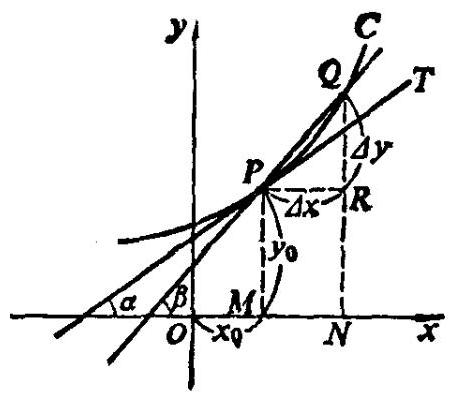
\includegraphics[max width=0.5\textwidth]{images/01912c18-5c3f-733d-b775-749ba9897a9d_62_329591.jpg}
\end{center}

图 2-1

这就是说, \(\frac{\Delta y}{\Delta x}\) 就是割线 \({PQ}\) 的斜率.

当点 \(Q\) 沿着曲线 \(O\) 无限地趋近于点 \(P\) ,即 \({\Delta x} \rightarrow 0\) 时,割线 \({PQ}\) 绕着点 \(P\) 转动,它的极限位置 \({PT}\) 叫做曲线 \(C\) 在点 \(P\) 处的切线. 这时如果函数 \(y = f\left( x\right)\) 在点 \({x}_{0}\) 处可导,那么当 \({\Delta x} \rightarrow 0\) 时, \(\frac{\Delta y}{\Delta x} \rightarrow {f}^{\prime }\left( {x}_{0}\right)\) ,而 \(\operatorname{tg}\beta\) 以 \({PT}\) 的斜率 \(\operatorname{tg}\alpha (\alpha\) 是 \({PT}\) 的倾斜角) 为极限, 所以

\[
{f}^{\prime }\left( {x}_{0}\right) = \operatorname{tg}\alpha \text{. }
\]

因此,函数 \(y = f\left( x\right)\) 在点 \({x}_{0}\) 处的导数 \({f}^{\prime }\left( {x}_{0}\right)\) 的几何意义,就是曲线 \(y = f\left( x\right)\) 在点 \(\left( {{x}_{0},f\left( {x}_{0}\right) }\right)\) 处的切线的斜率.

这样,求曲线 \(y = f\left( x\right)\) 在点 \(\left( {{x}_{0},f\left( {x}_{0}\right) }\right)\) 处的切线,只要先求出函数 \(y = f\left( x\right)\) 在点 \({x}_{0}\) 处的导数 \({f}^{\prime }\left( {x}_{0}\right)\) ,然后根据直线方程的点斜式, 就得到切线的方程

\[
y - {y}_{0} = {f}^{\prime }\left( {x}_{0}\right) \left( {x - {x}_{0}}\right)
\]

这里 \({y}_{0} = f\left( {x}_{0}\right)\) ,下同.

当 \(\alpha = \frac{\pi }{2}\) 时,导数不存在,这时切线 \({PT}\) 平行于 \(y\) 轴,切线的方程为

\[
x = {x}_{0}
\]

经过点 \(P\) 且和切线 \({PT}\) 垂直的直线叫做曲线 \(C\) 在点 \(P\) 处的法线. 由解析几何得知, 如果两条有斜率的直线互相垂直, 那么,它们的斜率互为负倒数. 已知曲线 \(y = f\left( x\right)\) 在点 \(\left( {x}_{0}\right.\) , \(\left. {f\left( {x}_{0}\right) }\right)\) 处的切线的斜率为 \({f}^{\prime }\left( {x}_{0}\right)\) ,那么,当 \({f}^{\prime }\left( {x}_{0}\right) \neq 0\) 时,曲线在该点处的法线的斜率为 \(- \frac{1}{{f}^{\prime }\left( {x}_{0}\right) }\) ,法线的方程为

\[
y - {y}_{0} = - \frac{1}{{f}^{\prime }\left( {x}_{0}\right) }\left( {x - {x}_{0}}\right) .
\]

当 \({f}^{\prime }\left( {x}_{0}\right) = 0\) 时,法线平行于 \(y\) 轴,法线的方程为

\[
x = {x}_{0}
\]

当切线 \({PT}\) 平行于 \(y\) 轴时,法线平行于 \(x\) 轴,这时法线的方程为

\[
y = {y}_{0}
\]

例 已知曲线 \(y = \frac{1}{3}{x}^{3}\) 上一点 \(P\left( {2,\frac{8}{3}}\right)\) . 求: (1) 过 \(P\) 点的切线的斜率; (2) 过 \(P\) 点的切线的方程; (3) 过 \(P\) 点的法线的方程.

解: (1) \(y = \frac{1}{3}{x}^{3}\) ,

\[
\therefore \;{y}^{\prime } = \mathop{\lim }\limits_{{{\Delta x} \rightarrow 0}}\frac{\Delta y}{\Delta x}
\]

\[
= \mathop{\lim }\limits_{{{\Delta x} \rightarrow 0}}\frac{\frac{1}{3}{\left( x + \Delta x\right) }^{3} - \frac{1}{3}{x}^{3}}{\Delta x}
\]

\[
= \frac{1}{3}\mathop{\lim }\limits_{{{\Delta x} \rightarrow 0}}\frac{3{x}^{2}{\Delta x} + {3x}{\left( \Delta x\right) }^{2} + {\left( \Delta x\right) }^{3}}{\Delta x}
\]

\[
= \frac{1}{3}\mathop{\lim }\limits_{{{\Delta x} \rightarrow 0}}\left\lbrack {3{x}^{2} + {3x\Delta x} + {\left( \Delta x\right) }^{2}}\right\rbrack
\]

\[
= {x}^{2}
\]

\[
{\left. {y}^{\prime }\right| }_{x = 2} = {2}^{2} = 4\text{. }
\]

\(\therefore\) 在点 \(P\) 处的切线的斜率等于 4 .

(2)在点 \(P\) 处的切线的方程为

\[
y - \frac{8}{3} = 4\left( {x - 2}\right)
\]

即

\[
{12x} - {3y} - {16} = 0.
\]

(3)在点 \(P\) 处的法线的方程为

\[
y - \frac{8}{3} = - \frac{1}{4}\left( {x - 2}\right)
\]

即

\[
{3x} + {12y} - {38} = 0\text{. }
\]

图形如图 2-2.

\begin{center}
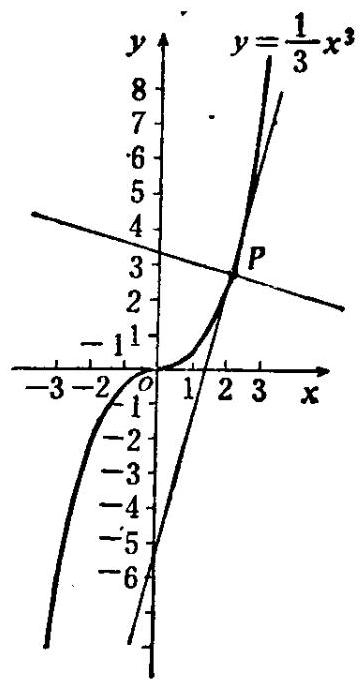
\includegraphics[max width=0.4\textwidth]{images/01912c18-5c3f-733d-b775-749ba9897a9d_65_242214.jpg}
\end{center}

图 2-2

\begin{problemset}[练习]

\item 求抛物线 \(y = {4x} - {x}^{2}\) 在点 \(A\left( {4,0}\right)\) 和点 \(B\left( {2,4}\right)\) 处的 \(\left( 1\right)\) 切线的斜率; (2) 切线的方程.

\item 求等边双曲线 \(y = \frac{9}{x}\) 在点 \(M\left( {3,3}\right)\) 处的切线的斜率与倾斜角。

\item 求抛物线 \(y = {x}^{2} + 2\) 在点 \(M\left( {2,6}\right)\) 处的切线方程和法线方程。

\end{problemset}

\section*{*变化率举例}

我们知道,函数 \(y = f\left( x\right)\) 的导数 \({f}^{\prime }\left( x\right)\) 就是函数对自变量 \(x\) 的变化率,因此,很多非均匀变化的变化率问题都可以应用导数来研究. 为了更好地理解和应用导数概念, 我们再举几个非均匀变化的变化率的例子.

例 1 瞬时功率.

已知物体所作的功 \(W\) 是时间 \(t\) 的函数: \(W = W\left( t\right)\) . 求在时刻 \(t = {t}_{0}\) 的功率.

分析: 功率表示作功的效率, 物体在某段时间内所作的功 \({\Delta W}\) 和这段时间 \({\Delta t}\) 的比 \(\frac{\Delta W}{\Delta t}\) ,就是这段时间内的(平均) 功率. 如果物体所作的功随时间增加而均匀改变, 这个比是个常数, 这个常数就是任一时刻的功率. 但是, 如果物体作功随时间的变化是非均匀的,那么, \(\frac{\Delta W}{\Delta t}\) 只表示某段时间内的平均功率. 因此,要求任一时刻 \({t}_{0}\) 的功率,就是求 \(\left\lbrack {{t}_{0},{t}_{0} + {\Delta t}}\right\rbrack\) 内的平均功率 \(\frac{\Delta W}{\Delta t}\) 当 \({\Delta t} \rightarrow 0\) 时的极限一瞬时功率.

解: 已知物体从 0 到 \(t\) 这段时间内所作的功是 \(W =\) \(W\left( t\right)\) ,那么,从时刻 \({t}_{0}\) 到 \({t}_{0} + {\Delta t}\) 这段时间内物体所作的功 (即功的改变量)为

\[
{\Delta W} = W\left( {{t}_{0} + {\Delta t}}\right) - W\left( {t}_{0}\right) .
\]

它和完成这些功所用时间(即时间改变量) \({\Delta t}\) 的比

\[
\frac{\Delta W}{\Delta t} = \frac{W\left( {{t}_{0} + {\Delta t}}\right) - W\left( {t}_{0}\right) }{\Delta t}
\]

就是 \({t}_{0}\) 到 \({t}_{0} + {\Delta t}\) 这段时间内的平均功率.

当 \({\Delta t} \rightarrow 0\) 时,平均功率的极限

\[
\mathop{\lim }\limits_{{{\Delta t} \rightarrow 0}}\frac{W\left( {{t}_{0} + {\Delta t}}\right) - W\left( {t}_{0}\right) }{\Delta t} = {P}_{0}
\]

就是在时刻 \({t}_{0}\) 的瞬时功率.

因此,功率 \(P\) 是功 \(W\) 对时间 \(t\) 的导数,即

\[
P = {W}^{\prime }\left( t\right)
\]

例 2 瞬时电流强度.

设有一随时间而变化的电流,从 0 到 \(t\) 这段时间内通过导线横截面的电量为 \(q = q\left( t\right)\) . 求在时刻 \({t}_{0}\) 时导线中的电流强度.

分析: 电流强度表示电流的强弱, 在某段时间内通过导线横截面的电量 \({\Delta q}\) 和这段时间 \({\Delta t}\) 的比 \(\frac{\Delta q}{\Delta t}\) ,就是这段时间内的电流强度. 如果给出的电流是稳恒电流,比 \(\frac{\Delta q}{\Delta t}\) 是一个常数, 这个常数就是任一时刻的电流强度. 但是, 如果电路中电流的强弱是变化的,那么, \(\frac{\Delta q}{\Delta t}\) 只表示某段时间内的平均电流强度. 因此,要求在时刻 \({t}_{0}\) 的电流强度,就是求 \(\left\lbrack {{t}_{0},{t}_{0} + {\Delta t}}\right\rbrack\) 内的平均电流强度 \(\frac{\Delta q}{\Delta t}\) 当 \({\Delta t} \rightarrow 0\) 时的极限一瞬时电流强度.

解: 已知从 0 到 \(t\) 这段时间内通过导线横截面的电量为 \(q\left( t\right)\) ,那么,从时刻 \({t}_{0}\) 到 \({t}_{0} + {\Delta t}\) 这段时间内通过导线横截面的电量为

\[
{\Delta q} = q\left( {{t}_{0} + {\Delta t}}\right) - q\left( {t}_{0}\right)
\]

这段时间内的平均电流强度为

\[
\frac{\Delta q}{\Delta t} = \frac{q\left( {{t}_{0} + {\Delta t}}\right) - q\left( {t}_{0}\right) }{\Delta t}.
\]

当 \({\Delta t} \rightarrow 0\) 时,平均电流强度的极限

\[
\mathop{\lim }\limits_{{{\Delta t} \rightarrow 0}}\frac{q\left( {{t}_{0} + {\Delta t}}\right) - q\left( {t}_{0}\right) }{\Delta t} = {I}_{0}
\]

就是在时刻 \({t}_{0}\) 的电流强度.

因此,电流强度 \(I\) 是电量 \(q\) 对时间 \(t\) 的导数,即

\[
I = {q}^{\prime }\left( t\right)
\]

\begin{problemset}[练习]

\item 在匀速圆周运动中, 连结运动质点和圆心的半径转过的角度和所用时间的比值, 叫做匀速圆周运动的角速度. 现有一质点作变速圆周运动,已知在时刻 \(t\) 连结运动质点和圆心的半径转过的角度为 \(\varphi \left( t\right)\) ,求它在时 刻 \({t}_{0}\) 的角速度 \({\omega }_{0}\) .

\item 某物质在一个化学反应中的浓度 \(C\) 与反应开始后的时间 \(t\) 之间的函数关系为 \(C = C\left( t\right)\) ,写出 \(t = a\) 时浓度的变化率。

\item 求导数的方法适用不适用于求均匀变化的量的变化率? 这时, 平均变化率和瞬时变化率有什么关系? 试加说明.

\end{problemset}

\section{函数的可导性与连续性的关系}

由导数的定义, 可以推出函数在一点处可导与函数在该点处连续的关系:

如果函数 \(y = f\left( x\right)\) 在点 \({x}_{0}\) 处可导,那么 \(y = f\left( x\right)\) 在点 \({x}_{0}\) 处连续.

证明 我们是要根据

\[
\mathop{\lim }\limits_{{{\Delta x} \rightarrow 0}}\frac{f\left( {{x}_{0} + {\Delta x}}\right) - f\left( {x}_{0}\right) }{\Delta x} = {f}^{\prime }\left( {x}_{0}\right)
\]

来证明

\[
\mathop{\lim }\limits_{{x \rightarrow {x}_{0}}}f\left( x\right) = f\left( {x}_{0}\right) .
\]

考虑 \(\mathop{\lim }\limits_{{x \rightarrow {x}_{0}}}f\left( x\right)\) ,令 \(x = {x}_{0} + {\Delta x},x \rightarrow {x}_{0}\) 相当于 \({\Delta x} \rightarrow 0\) ,于是

\[
\mathop{\lim }\limits_{{x \rightarrow {x}_{0}}}f\left( x\right) = \mathop{\lim }\limits_{{{\Delta x} \rightarrow 0}}f\left( {{x}_{0} + {\Delta x}}\right)
\]

\[
= \mathop{\lim }\limits_{{{\Delta x} \rightarrow 0}}\left\lbrack {f\left( {{x}_{0} + {\Delta x}}\right) - f\left( {x}_{0}\right) + f\left( {x}_{0}\right) }\right\rbrack
\]

\[
= \mathop{\lim }\limits_{{{\Delta x} \rightarrow 0}}\left\lbrack {\frac{f\left( {{x}_{0} + {\Delta x}}\right) - f\left( {x}_{0}\right) }{\Delta x} \cdot {\Delta x} + f\left( {x}_{0}\right) }\right\rbrack
\]

\[
= \mathop{\lim }\limits_{{{\Delta x} \rightarrow 0}}\frac{f\left( {{x}_{0} + {\Delta x}}\right) - f\left( {x}_{0}\right) }{\Delta x} \cdot {\Delta x} + f\left( {x}_{0}\right)
\]

\[
= \mathop{\lim }\limits_{{{\Delta x} \rightarrow 0}}\frac{f\left( {{x}_{0} + {\Delta x}}\right) - f\left( {x}_{0}\right) }{\Delta x} \cdot \mathop{\lim }\limits_{{{\Delta x} \rightarrow 0}}{\Delta x} + f\left( {x}_{0}\right)
\]

\[
= {f}^{\prime }\left( {x}_{0}\right) \cdot 0 + f\left( {x}_{0}\right)
\]

\[
= f\left( {x}_{0}\right) \text{.}
\]

但是,如果函数 \(f\left( x\right)\) 在点 \({x}_{0}\) 连续, \(f\left( x\right)\) 在该点不一定可导. 例如 \(y = \left| x\right|\) 在点 \(x = 0\) 连续,但在点 \(x = 0\) 处不可导. 从图形上看,就是曲线 \(y = f\left( x\right)\) 在点 \(O\left( {0,0}\right)\) 处没有切线 (图 \(2 - 3)\) .

\begin{center}
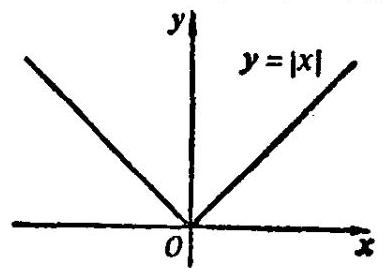
\includegraphics[max width=0.4\textwidth]{images/01912c18-5c3f-733d-b775-749ba9897a9d_69_933568.jpg}
\end{center}

图 2-3

*下面我们根据导数的定义证明 \(y = \left| x\right|\) 在 \(x = 0\) 处不可导. 并从而导出左、右导数的概念.

\(\because {\Delta y} = \left| {0 + {\Delta x}}\right| - \left| 0\right| = \left| {\Delta x}\right| = \left\{ \begin{array}{r} {\Delta x},\text{ 当 }{\Delta x} > 0, \\ - {\Delta x},\text{ 当 }{\Delta x} < 0, \end{array}\right.\)

\[
\therefore \mathop{\lim }\limits_{{{\Delta x} \rightarrow 0 + }}\frac{\Delta y}{\Delta x} = \mathop{\lim }\limits_{{{\Delta x} \rightarrow 0 + }}\frac{\Delta x}{\Delta x} = 1\text{,}
\]

\[
\mathop{\lim }\limits_{{{\Delta x} \rightarrow 0 - }}\frac{\Delta y}{\Delta x} = \mathop{\lim }\limits_{{{\Delta x} \rightarrow 0 - }}\frac{-{\Delta x}}{\Delta x} = - 1.
\]

也就是说,当 \({\Delta x} \rightarrow 0\) 时, \(\frac{\Delta y}{\Delta x}\) 的左、右极限不相等,所以 \(\frac{\Delta y}{\Delta x}\) 当 \({\Delta x} \rightarrow 0\) 时极限 不存在. 因此,函数 \(y = \left| x\right|\) 在点 \(x = 0\) 处不可导.

一般地,设已知函数 \(y = f\left( x\right) ,{\Delta y} = f\left( {{x}_{0} + {\Delta x}}\right) - f\left( {x}_{0}\right)\) ,如果 \(\frac{\Delta y}{\Delta x}\) 的左极限存在,就把左极限 \(\mathop{\lim }\limits_{{{\Delta x} \rightarrow 0}}\frac{\Delta y}{\Delta x}\) 叫做 \(f\left( x\right)\) 在点 \({x}_{0}\) 处的左导数; 如果 \(\frac{\Delta y}{\Delta x}\) 的右极限存在,就把右极限 \(\mathop{\lim }\limits_{{{\Delta x} \rightarrow 0 + }}\frac{\Delta y}{\Delta x}\) 叫做 \(f\left( x\right)\) 在点 \({x}_{0}\) 处的右导数.

根据左、右极限存在且相等是极限存在的充要条件, 可得左、右导数存在且相等是导数存在的充要条件.

如果函数 \(y = f\left( x\right)\) 在开区间 \(\left( {a,b}\right)\) 内可导,在左端点 \(x =\) \(a\) 处存在右导数,在右端点 \(x = b\) 处存在左导数,我们就说函数 \(f\left( x\right)\) 在闭区间 \(\left\lbrack {a,b}\right\rbrack\) 上可导.

\begin{problemset}[练习]

\item 先从函数的图象观察,然后根据定义判断函数 \(y = \sqrt[3]{{x}^{2}}\) 在点 \(x = 0\) 处是否连续,在点 \(x = 0\) 处是否可导.

\end{problemset}

\begin{problemset}[习 题 四]

\item 已知作直线运动的某一物体的运动方程为 \(s = \frac{5}{2}{t}^{2}\) (米), 当 \(t = 2\) 秒, \({\Delta t}\) 分别为 0.1 秒、 0.01 秒、 0.001 秒、 0.0001 秒、0.00001 秒时,求从 \({t}_{0}\) 到 \({t}_{0} + {\Delta t}\) 这段时间内的平均速度及 \(t = 2\) 秒时的瞬时速度.

\item 已知质点按规律 \(s = 2{t}^{2} + {4t}\) (米) 作直线运动,求:

(1)质点在运动开始后前 3 秒内的平均速度;

(2)质点在 2 秒到 3 秒内的平均速度;

(3)质点在 3 秒时的瞬时速度。

\item 求下列函数在指定点处的导数:

(1) \(y = {\left( x - 2\right) }^{2}\) ,点 \(x = 2\) ; (2) \(y = \frac{1}{x - 1}\) ,点 \(x = 0\) .

\item 说明函数 \(y = f\left( x\right)\) 在点 \({x}_{0}\) 处的导数也可定义为

\[
{f}^{\prime }\left( {x}_{0}\right) = \mathop{\lim }\limits_{{x \rightarrow {x}_{0}}}\frac{f\left( x\right) - f\left( {x}_{0}\right) }{x - {x}_{0}}.
\]

\item 求下列函数的导数:

(1) \(y = {ax} + b\) ; (2) \(y = \frac{1}{x}\)

(3) \(y = \frac{1}{{x}^{2}}\) (4) \(y = \frac{1}{\sqrt{x}}\) .

\item 已知 \(f\left( x\right) = \frac{1}{1 - x}\) ,求 \({f}^{\prime }\left( x\right) ,{f}^{\prime }\left( 0\right) ,{f}^{\prime }\left( 2\right)\) .

\item 已知 \(y = \sqrt{{a}^{2} - {x}^{2}}\) ,求证 \({y}^{\prime } = - \frac{x}{\sqrt{{a}^{2} - {x}^{2}}}\) .

\item 设质点 \(M\) 沿 \(x\) 轴作变速直线运动,在时刻 \(t\) (秒),质点 \(M\)

所在位置为 \(x = {t}^{2} - {5t} + 6\) (米). 求从 1 秒到 3 秒 这段时间内质点 \(M\) 的平均速度. 质点 \(M\) 在什么时刻的速度等于这段时间内的平均速度?

\item 求曲线 \(y = {2x} - {x}^{3}\) 在点 \(\left( {-1, - 1}\right)\) 处的切线的倾斜角.

\item 求抛物线 \(y = \frac{1}{4}{x}^{2}\) 在点 \(\left( {-2,1}\right)\) 及点 \(\left( {2,1}\right)\) 处的切线方程和法线方程。

\item 从时刻 \(t = 0\) 开始的 \(t\) 秒内,通过某导体的电量 (单位: 库仑)可由公式 \(q = 2{t}^{2} + {3t}\) 表示. 求第 5 秒时的电流强度及第 7 秒时的电流强度(即通过的电量 \(q\) 对时间 \(t\) 的导数 \({q}_{t}^{\prime }\) ),什么时刻电流强度达到 43 安培 (即库仑/秒).

\end{problemset}

\section*{求 导 方 法}

\section{几种常见函数的导数}

为了能够较快地求出某个函数的导数, 在下几节中我们将研究求导数的一般运算法则以及基本初等函数的导数公式. 这一节, 我们根据导数的定义先来证明几个常见函数的导数公式.

1. 设 \(y = C\) ( \(C\) 为常数),则 \({y}^{\prime } = 0\) .

证明:

\[
y = f\left( x\right) = C,
\]

\[
{\Delta y} = f\left( {x + {\Delta x}}\right) - f\left( x\right)
\]

\[
= C - C = 0,
\]

\[
\frac{\Delta y}{\Delta x} = 0
\]

\(\therefore \;{f}^{\prime }\left( x\right) = {C}^{\prime } = \mathop{\lim }\limits_{{{\Delta x} \rightarrow 0}}\frac{\Delta y}{\Delta x} = 0\) .

2. \({\left( {x}^{n}\right) }^{\prime } = n{x}^{n - 1}\) ( \(n\) 为正整数)

证明: \(y = f\left( x\right) = {x}^{n}\) ,

\[
{\Delta y} = f\left( {x + {\Delta x}}\right) - f\left( x\right)
\]

\[
= {\left( x + \Delta x\right) }^{n} - {x}^{n}
\]

\[
= \left\lbrack {{x}^{n} + {C}_{n}^{1}{x}^{n - 1}{\Delta x} + {C}_{n}^{2}{x}^{n - 2}{\left( \Delta x\right) }^{2}}\right.
\]

\[
\left. {+\cdots + {C}_{n}^{n}{\left( \Delta x\right) }^{n}}\right\rbrack - {x}^{n}
\]

\[
= {C}_{n}^{1}{x}^{n - 1}{\Delta x} + {C}_{n}^{2}{x}^{n - 2}{\left( \Delta x\right) }^{2} + \cdots + {C}_{n}^{n}{\left( \Delta x\right) }^{n},
\]

\[
\frac{\Delta y}{\Delta x} = {C}_{n}^{1}{x}^{n - 1} + {C}_{n}^{2}{x}^{n - 2}{\Delta x} + \cdots + {C}_{n}^{n}{\left( \Delta x\right) }^{n - 1},
\]

\[
\therefore \;{y}^{\prime } = {\left( {x}^{n}\right) }^{\prime } = \mathop{\lim }\limits_{{{\Delta x} \rightarrow 0}}\frac{\Delta y}{\Delta x}
\]

\[
= \mathop{\lim }\limits_{{{\Delta x} \rightarrow 0}}\left\lbrack {{C}_{n}^{1}{x}^{n - 1} + {C}_{n}^{2}{x}^{n - 2}{\Delta x} + \cdots + {C}_{n}^{n}{\left( \Delta x\right) }^{n - 1}}\right\rbrack
\]

\[
= n{x}^{n - 1}\text{. }
\]

例如,

\[
{\left( {x}^{3}\right) }^{\prime } = 3{x}^{2},\;{\left( {x}^{7}\right) }^{\prime } = 7{x}^{6},\;{\left( x\right) }^{\prime } = 1{x}^{0} = 1.
\]

3. \({\left( \sin x\right) }^{\prime } = \cos x\)

证明: \(y = \sin x\) ,

\[
{\Delta y} = \sin \left( {x + {\Delta x}}\right) - \sin x = 2\cos \left( {x + \frac{\Delta x}{2}}\right) \sin \frac{\Delta x}{2},
\]

\[
\frac{\Delta y}{\Delta x} = \cos \left( {x + \frac{\Delta x}{2}}\right) \frac{\sin \frac{\Delta x}{2}}{\frac{\Delta x}{2}}
\]

\(\because \;\mathop{\lim }\limits_{{{\Delta x} \rightarrow 0}}\frac{\sin \frac{\Delta x}{2}}{\frac{\Delta x}{2}} = 1\)

\(\therefore \;{y}^{\prime } = {\left( \sin x\right) }^{\prime } = \mathop{\lim }\limits_{{{\Delta x} \rightarrow 0}}\frac{\Delta y}{\Delta x}\)

\[
= \mathop{\lim }\limits_{{{\Delta x} \rightarrow 0}}\cos \left( {x + \frac{\Delta x}{2}}\right) \cdot \mathop{\lim }\limits_{{{\Delta x} \rightarrow 0}}\frac{\sin \frac{\Delta x}{2}}{\frac{\Delta x}{2}} = \cos x.
\]

4. \({\left( \cos x\right) }^{\prime } = - \sin x\)

请同学自己证明.

\begin{problemset}[练习]

\item (口答) 求下列函数的导数:

(1) \(y = {x}^{5}\) ; (2) \(y = {x}^{6}\) ;

(3) \(x = \sin t\) ; (4) \(u = \cos \varphi\) .

\end{problemset}

\section{函数的和、差、积、商的导数}

相应于函数极限的四则运算法则, 我们根据导数的定义来导出求导数的四则运算法则, 以简化求导数的计算. 在下面的公式中, \(u\) 及 \(v\) 都是 \(x\) 的函数,而且都是可导的.

\section*{1. 和(或差)的导数}

法则 1 两个函数的和 (或差) 的导数, 等于这两个函数的导数的和(或差). 即

\[
{\left( \mathbf{u} \pm \mathbf{v}\right) }^{\prime } = {\mathbf{u}}^{\prime } \pm \mathbf{v}.
\]

证明: \(y = f\left( x\right) = u\left( x\right) \pm v\left( x\right)\) ,

\[
{\Delta y} = \left\lbrack {u\left( {x + {\Delta x}}\right) \pm v\left( {x + {\Delta x}}\right) }\right\rbrack - \left\lbrack {u\left( x\right) \pm v\left( x\right) }\right\rbrack
\]

\[
= \left\lbrack {u\left( {x + {\Delta x}}\right) - u\left( x\right) }\right\rbrack \pm \left\lbrack {v\left( {x + {\Delta x}}\right) - v\left( x\right) }\right\rbrack
\]

\[
= {\Delta u} \pm {\Delta v}
\]

\[
\frac{\Delta y}{\Delta x} = \frac{\Delta u}{\Delta x} \pm \frac{\Delta v}{\Delta x}
\]

\[
\mathop{\lim }\limits_{{{\Delta x} \rightarrow 0}}\frac{\Delta y}{\Delta x} = \mathop{\lim }\limits_{{{\Delta x} \rightarrow 0}}\left( {\frac{\Delta u}{\Delta x} \pm \frac{\Delta v}{\Delta x}}\right) = \mathop{\lim }\limits_{{{\Delta x} \rightarrow 0}}\frac{\Delta u}{\Delta x} \pm \mathop{\lim }\limits_{{{\Delta x} \rightarrow 0}}\frac{\Delta v}{\Delta x}
\]

即

\[
{y}^{\prime } = {\left( u \pm v\right) }^{\prime } = {u}^{\prime } \pm {v}^{\prime }.
\]

这个法则可以推广到任意有限个函数, 即

\[
{\left( {u}_{1} \pm {u}_{2} \pm \cdots \pm {u}_{n}\right) }^{\prime } = {u}_{1}^{\prime } \pm {u}_{2}^{\prime } \pm \cdots \pm {u}_{n}^{\prime }.
\]

例 1 求 \(y = {x}^{3} + \sin x\) 的导数.

解: \({y}^{\prime } = {\left( {x}^{3}\right) }^{\prime } + {\left( \sin x\right) }^{\prime } = 3{x}^{2} + \cos x\) .

例 2 求 \(y = {x}^{4} - {x}^{2} - x + 3\) 的导数.

解: \({y}^{\prime } = 4{x}^{3} - {2x} - 1\) .

\section*{2. 积的导数}

法则 2 两个函数的积的导数, 等于第一个函数的导数乘以第二个函数, 加上第一个函数乘以第二个函数的导数. 即

\[
{\left( uv\right) }^{\prime } = {u}^{\prime }v + u{v}^{\prime }
\]

证明: \(y = f\left( x\right) = u\left( x\right) v\left( x\right)\) ,

\[
{\Delta y} = u\left( {x + {\Delta x}}\right) v\left( {x + {\Delta x}}\right) - u\left( x\right) v\left( x\right)
\]

\[
= u\left( {x + {\Delta x}}\right) v\left( {x + {\Delta x}}\right) - u\left( x\right) v\left( {x + {\Delta x}}\right)
\]

\[
+ u\left( x\right) v\left( {x + {\Delta x}}\right) - u\left( x\right) v\left( x\right)
\]

\[
\frac{\Delta y}{\Delta x} = \frac{u\left( {x + {\Delta x}}\right) - u\left( x\right) }{\Delta x}v\left( {x + {\Delta x}}\right) + u\left( x\right) \frac{v\left( {x + {\Delta x}}\right) - v\left( x\right) }{\Delta x}.
\]

因为 \(v\left( x\right)\) 在点 \(x\) 处可导,所以它在点 \(x\) 处连续,于是当 \({\Delta x} \rightarrow 0\) 时, \(v\left( {x + {\Delta x}}\right) \rightarrow v\left( x\right)\) . 从而

\[
\mathop{\lim }\limits_{{{\Delta x} \rightarrow 0}}\frac{\Delta y}{\Delta x} = \mathop{\lim }\limits_{{{\Delta x} \rightarrow 0}}\frac{u\left( {x + {\Delta x}}\right) - u\left( x\right) }{\Delta x}v\left( {x + {\Delta x}}\right)
\]

\[
+ u\left( x\right) \mathop{\lim }\limits_{{{\Delta x} \rightarrow 0}}\frac{v\left( {x + {\Delta x}}\right) - v\left( x\right) }{\Delta x}
\]

\[
= {u}^{\prime }v + u{v}^{\prime }
\]

即

\[
{y}^{\prime } = {\left( uv\right) }^{\prime } = {u}^{\prime }v + u{v}^{\prime }.
\]

从法则 2 立即可以得出

\[
{\left( Cu\right) }^{\prime } = {C}^{\prime }u + C{u}^{\prime } = 0 + C{u}^{\prime } = C{u}^{\prime },
\]

也就是, 常数与函数的积的导数, 等于常数乘以函数的导数.

即

\[
{\left( Cu\right) }^{\prime } = C{u}^{\prime }\text{. }
\]

例 3 求 \(y = 2{x}^{3} - 3{x}^{2} + {5x} - 4\) 的导数.

解: \({y}^{\prime } = 6{x}^{2} - {6x} + 5\) .

例 4 求 \(y = \left( {2{x}^{2} + 3}\right) \left( {{3x} - 2}\right)\) 的导数.

解: \({y}^{\prime } = {\left( 2{x}^{2} + 3\right) }^{\prime }\left( {{3x} - 2}\right) + \left( {2{x}^{2} + 3}\right) {\left( 3x - 2\right) }^{\prime }\)

\[
= {4x} \cdot \left( {{3x} - 2}\right) + \left( {2{x}^{2} + 3}\right) \cdot 3 = {18}{x}^{2} - {8x} + 9\text{.}
\]

\section*{3. 商的导数}

法则 3 两个函数的商的导数, 等于分子的导数 与分母的积, 减去分母的导数与分子的积, 再除以分母的平方. 即

\[
{\left( \frac{u}{v}\right) }^{\prime } = \frac{{u}^{\prime }v - u{v}^{\prime }}{{v}^{2}}\;\left( {v \neq 0}\right) .
\]

证明: \(y = f\left( x\right) = \frac{u\left( x\right) }{v\left( x\right) }\) ,

\[
{\Delta y} = \frac{u\left( {x + {\Delta x}}\right) }{v\left( {x + {\Delta x}}\right) } - \frac{u\left( x\right) }{v\left( x\right) }
\]

\[
= \frac{u\left( {x + {\Delta x}}\right) v\left( x\right) - u\left( x\right) v\left( {x + {\Delta x}}\right) }{v\left( {x + {\Delta x}}\right) v\left( x\right) }
\]

\[
= \frac{\left\lbrack {u\left( {x + {\Delta x}}\right) v\left( x\right) - u\left( x\right) v\left( x\right) }\right\rbrack - \left\lbrack {u\left( x\right) v\left( {x + {\Delta x}}\right) - u\left( x\right) v\left( x\right) }\right\rbrack }{v\left( {x + {\Delta x}}\right) v\left( x\right) }
\]

\[
= \frac{\left\lbrack {u\left( {x + {\Delta x}}\right) - u\left( x\right) }\right\rbrack v\left( x\right) - u\left( x\right) \left\lbrack {v\left( {x + {\Delta x}}\right) - v\left( x\right) }\right\rbrack }{v\left( {x + {\Delta x}}\right) v\left( x\right) }.
\]

\[
\frac{\Delta y}{\Delta x} = \frac{\frac{u\left( {x + {\Delta x}}\right) - u\left( x\right) }{\Delta x}v\left( x\right) - u\left( x\right) \frac{v\left( {x + {\Delta x}}\right) - v\left( x\right) }{\Delta x}}{v\left( {x + {\Delta x}}\right) v\left( x\right) }.
\]

因为 \(v\left( x\right)\) 在点 \(x\) 处可导,所以它在点 \(x\) 处连续,于是当 \({\Delta x} \rightarrow 0\) 时, \(v\left( {x + {\Delta x}}\right) \rightarrow v\left( x\right)\) . 从而

\[
\mathop{\lim }\limits_{{{\Delta x} \rightarrow 0}}\frac{\Delta y}{\Delta x} = \frac{{u}^{\prime }\left( x\right) v\left( x\right) - u\left( x\right) {v}^{\prime }\left( x\right) }{{\left\lbrack v\left( x\right) \right\rbrack }^{2}},
\]

即

\[
{y}^{\prime } = {\left( \frac{u}{v}\right) }^{\prime } = \frac{{u}^{\prime }v - u{v}^{\prime }}{{v}^{2}}.
\]

例 5 求 \(y = \frac{{x}^{2}}{\sin x}\) 的导数.

解: \({y}^{\prime } = \frac{{\left( {x}^{2}\right) }^{\prime } \cdot \sin x - {x}^{2} \cdot {\left( \sin x\right) }^{\prime }}{{\sin }^{2}x} = \frac{{2x}\sin x - {x}^{2}\cos x}{{\sin }^{2}x}\) .

例 6 求 \(y = \frac{x + 3}{{x}^{2} + 3}\) 在点 \(x = 3\) 处的导数.

解: \({y}^{\prime } = \frac{1 \cdot \left( {{x}^{2} + 3}\right) - \left( {x + 3}\right) \cdot {2x}}{{\left( {x}^{2} + 3\right) }^{2}} = \frac{-{x}^{2} - {6x} + 3}{{\left( {x}^{2} + 3\right) }^{2}}\) ,

\[
\therefore {\left. {y}^{\prime }\right| }_{x = 3} = \frac{-9 - {18} + 3}{{\left( 9 + 3\right) }^{2}} = \frac{-{24}}{144} = - \frac{1}{6}\text{.}
\]

例 7 求证当 \(n\) 是负整数时,公式

\[
{\left( {x}^{n}\right) }^{\prime } = n{x}^{n - 1}
\]

仍然成立.

证明: 设 \(n = - m\) ,则 \(m\) 为正整数.

\[
\therefore \;{\left( {x}^{n}\right) }^{\prime } = {\left( {x}^{-m}\right) }^{\prime } = {\left( \frac{1}{{x}^{m}}\right) }^{\prime }
\]

\[
= \frac{0 \cdot {x}^{m} - m{x}^{m - 1}}{{x}^{2m}}
\]

\[
= - m{x}^{-m - 1} = n{x}^{n - 1}.
\]

例 8 求 \(y = 2{x}^{2} - {3x} + 4 - \frac{3}{x} + \frac{2}{{x}^{2}}\) 的导数.

解: \(y = 2{x}^{2} - {3x} + 4 - 3{x}^{-1} + 2{x}^{-2}\) ,

\[
\therefore \;{y}^{\prime } = {4x} - 3 + 3{x}^{-2} - 4{x}^{-3}
\]

\[
= {4x} - 3 + \frac{3}{{x}^{2}} - \frac{4}{{x}^{3}}
\]

\begin{problemset}[练习]

\item 求下列函数的导数:

(1) \(y = 3{x}^{4} - {23}{x}^{3} + {40x} - {10}\) ; \(\;\left( 2\right) y = a{x}^{3} - {bx} + c\) ;

(3) \(y = \sin x - x + 1\) ; (4) \(y = {x}^{2} + 2\cos x\) .

\item 填空:

(1) \({\left\lbrack \left( 3{x}^{2} + 1\right) \left( 4{x}^{2} - 3\right) \right\rbrack }^{\prime }\)

\(= \left( \;\right) \left( {4{x}^{2} - 3}\right) + \left( {3{x}^{2} + 1}\right) \left( \;\right)\) ;

(2) \({\left( {x}^{3}\sin x\right) }^{\prime } = \left( \;\right) {x}^{2}\sin x + {x}^{3}\left( \;\right)\) .

\item 求下列函数的导数:

(1) \(y = \left( {3{x}^{2} + 1}\right) \left( {2 - x}\right)\) ; (2) \(y = \left( {1 - 2{x}^{3}}\right) \left( {x - 3{x}^{2}}\right)\) ;

(3) \(y = \left( {1 + {x}^{2}}\right) \cos x\) ; (4) \(y = \left( {1 + \sin x}\right) \left( {1 - {2x}}\right)\) .

\item 填空:

(1) \({\left( \frac{x}{{x}^{2} + 1}\right) }^{\prime } = \frac{\left( \;\right) \left( {{x}^{2} + 1}\right) - x\left( \;\right) }{{\left( {x}^{2} + 1\right) }^{2}}\)

(2) \({\left( \frac{1 - {x}^{2}}{\sin x}\right) }^{\prime } = \frac{\left( \;\right) \sin x - \left( {1 - {x}^{2}}\right) \left( \;\right) }{{\sin }^{2}x}\) .

\item 求下列函数的导数:

(1) \(y = \frac{a - x}{a + x}\) (2) \(y = \frac{1 + x}{3 - {x}^{2}}\)

(3) \(y = \frac{\cos x}{1 - {x}^{2}}\) (4) \(y = \frac{1}{1 + \sin x}\) ;

(5) \(y = 1 + \frac{2}{x} + \frac{3}{{x}^{2}} - \frac{4}{{x}^{3}}\) (6) \(y = \frac{-3{x}^{4} + 3{x}^{2} - 5}{{x}^{3}}\) .

\item 下列做法是否正确? 如果不正确, 加以改正:

(1) \({\left\lbrack \left( 3 + {x}^{2}\right) \left( 2 - {x}^{3}\right) \right\rbrack }^{\prime } = {2x}\left( {2 - {x}^{3}}\right) + 3{x}^{2}\left( {3 + {x}^{2}}\right)\) ;

(2) \({\left( \frac{1 + \cos x}{{x}^{2}}\right) }^{\prime } = \frac{{2x}\left( {1 + \cos x}\right) + {x}^{2}\sin x}{{x}^{2}}\) .

\end{problemset}

\section{复合函数的导数}

我们先看一个例子. 设已知

\[
y = {\left( 3x - 2\right) }^{2},
\]

那么,

\[
{y}^{\prime } = {\left\lbrack {\left( 3x - 2\right) }^{2}\right\rbrack }^{\prime } = {\left( 9{x}^{2} - {12}x + 4\right) }^{\prime } = {18x} - {12}.
\]

函数 \(y = {\left( 3x - 2\right) }^{2}\) 又可以看成由

\[
y = {u}^{2},u = {3x} - 2
\]

复合而成的. 由于

\[
{y}_{u}^{\prime } = {2u},\;{u}_{x}^{\prime } = 3,
\]

因而

\[
{y}_{u}^{\prime } \cdot {u}_{x}^{\prime } = {2u} \cdot 3 = 2\left( {{3x} - 2}\right) \cdot 3 = {18x} - {12}.
\]

于是在本例中, 我们有等式

\[
{y}_{x}^{\prime } = {y}_{u}^{\prime } \cdot {u}_{x}^{\prime }
\]

一般地,设函数 \(u = \varphi \left( x\right)\) 在点 \(x\) 处有导数 \({u}_{x}^{\prime } = {\varphi }^{\prime }\left( x\right)\) , 函数 \(y = f\left( u\right)\) 在点 \(x\) 的对应点 \(u\) 处有导数 \({y}_{u}^{\prime } = {f}^{\prime }\left( u\right)\) ,则复合函数 \(y = f\left\lbrack {\varphi \left( x\right) }\right\rbrack\) 在点 \(x\) 处也有导数,且

\[
{y}_{x}^{\prime } = {y}_{u}^{\prime } \cdot {u}_{x}^{\prime }
\]

或写作

\[
{f}_{x}^{\prime }\left\lbrack {\varphi \left( x\right) }\right\rbrack = {f}^{\prime }\left( u\right) {\varphi }^{\prime }\left( x\right) .
\]

证明: 设 \(x\) 有一改变量 \({\Delta x}\) ,则对应的 \(u\text{、}y\) 分别有改变量 \({\Delta u}\text{、}{\Delta y}\) . 因为 \(u = \varphi \left( x\right)\) 在点 \(x\) 处可导,所以 \(u = \varphi \left( x\right)\) 在点 \(x\) 处连续. 因此当 \({\Delta x} \rightarrow 0\) 时, \({\Delta u} \rightarrow 0\) . 设 \({\Delta u} \neq 0\mathbf{0}\) ,由

\[
\frac{\Delta y}{\Delta x} = \frac{\Delta y}{\Delta u} \cdot \frac{\Delta u}{\Delta x}
\]

且

\[
\mathop{\lim }\limits_{{{\Delta x} \rightarrow 0}}\frac{\Delta y}{\Delta u} = \mathop{\lim }\limits_{{{\Delta u} \rightarrow 0}}\frac{\Delta y}{\Delta u}
\]

得

\[
\mathop{\lim }\limits_{{{\Delta x} \rightarrow 0}}\frac{\Delta y}{\Delta x} = \mathop{\lim }\limits_{{{\Delta x} \rightarrow 0}}\frac{\Delta y}{\Delta u} \cdot \mathop{\lim }\limits_{{{\Delta x} \rightarrow 0}}\frac{\Delta u}{\Delta x}
\]

3 \({\Delta u} = 0\) 时公式也成立,证明从略.

\[
= \mathop{\lim }\limits_{{{\Delta u} \rightarrow 0}}\frac{\Delta y}{\Delta u} \cdot \mathop{\lim }\limits_{{{\Delta x} \rightarrow 0}}\frac{\Delta u}{\Delta x}
\]

即

\[
{y}_{x}^{\prime } = {y}_{u}^{\prime } \cdot {u}_{x}^{\prime }
\]

这就是复合函数的求导法则, 即: 复合函数对自变量的导数, 等于已知函数对中间变量的导数, 乘以中间变量对自变量的导数.

这个法则可以推广到两个以上的中间变量. 例如, 如果

\[
y = y\left( u\right) ,u = u\left( v\right) ,v = v\left( x\right) ,
\]

那么有

\[
{y}_{x}^{\prime } = {y}_{u}^{\prime } \cdot {u}_{v}^{\prime } \cdot {v}_{x}^{\prime }
\]

例 1 求 \(y = {\left( 2x + 1\right) }^{5}\) 的导数.

解: 设 \(y = {u}^{5},u = {2x} + 1\) .

根据复合函数求导法则, 有

\[
{y}_{x}^{\prime } = {y}_{u}^{\prime } \cdot {u}_{x}^{\prime } = {\left( {u}^{5}\right) }_{u}^{\prime } \cdot {\left( 2x + 1\right) }_{x}^{\prime }
\]

\[
= 5{u}^{4} \cdot 2 = 5{\left( 2x + 1\right) }^{4} \cdot 2
\]

\[
= {10}{\left( 2x + 1\right) }^{4}\text{.}
\]

注意: 在利用复合函数的求导法则求导数后, 要把中间变量换成自变量的函数.

例 2 求 \(y = \frac{1}{{\left( 1 - 3x\right) }^{4}}\) 的导数.

解: \(y = \frac{1}{{\left( 1 - 3x\right) }^{4}} = {\left( 1 - 3x\right) }^{-4}\) .

设 \(y = {u}^{-4},u = \left( {1 - {3x}}\right)\) ,则

\[
{y}_{x}^{\prime } = {y}_{u}^{\prime } \cdot {u}_{x}^{\prime }
\]

\[
= {\left( {u}^{-4}\right) }_{u}^{\prime } \cdot {\left( 1 - 3x\right) }_{x}^{\prime }
\]

\[
= - 4{u}^{-5} \cdot \left( {-3}\right)
\]

\[
= {12}{u}^{-5}
\]

\[
= {12}{\left( 1 - 3x\right) }^{-5}
\]

\[
= \frac{12}{{\left( 1 - 3x\right) }^{5}}
\]

例 3 求 \(y = {\sin }^{2}\left( {{2x} + \frac{\pi }{3}}\right)\) 的导数.

解: 设 \(y = {u}^{2},u = \sin v,v = {2x} + \frac{\pi }{3}\) ,

\[
{y}_{x}^{\prime } = {y}_{u}^{\prime } \cdot {u}_{v}^{\prime } \cdot {v}_{x}^{\prime }
\]

\[
= {\left( {u}^{2}\right) }_{u}^{\prime } \cdot {\left( \sin v\right) }_{v}^{\prime } \cdot {\left( 2x + \frac{\pi }{3}\right) }_{x}^{\prime }
\]

\[
= {2u} \cdot \cos v \cdot 2
\]

\[
= 2\sin \left( {{2x} + \frac{\pi }{3}}\right) \cdot \cos \left( {{2x} + \frac{\pi }{3}}\right) \cdot 2
\]

\[
= 2\sin \left( {{4x} + \frac{2\pi }{3}}\right) \text{.}
\]

求复合函数的导数, 关键在于分析清楚函数的复合关系, 适当选定中间变量, 明确每次是哪个变量对哪个变量求导数. 在熟练以后, 就不必再写出中间步骤. 如以上三例可分别直接写成

\[
{y}^{\prime } = {\left\lbrack {\left( 2x + 1\right) }^{5}\right\rbrack }^{\prime } = 5{\left( 2x + 1\right) }^{4} \cdot 2 = {10}{\left( 2x + 1\right) }^{4}.
\]

\[
{y}^{\prime } = {\left\lbrack {\left( 1 - 3x\right) }^{-4}\right\rbrack }^{\prime } = - 4{\left( 1 - 3x\right) }^{-5} \cdot \left( {-3}\right) = {12}{\left( 1 - 3x\right) }^{-5}.
\]

\[
{y}^{\prime } = {\left\lbrack {\sin }^{2}\left( 2x + \frac{\pi }{3}\right) \right\rbrack }^{\prime } = 2\sin \left( {{2x} + \frac{\pi }{3}}\right) \cdot \cos \left( {{2x} + \frac{\pi }{3}}\right) \cdot 2
\]

\[
= 2\sin \left( {{4x} + \frac{2\pi }{3}}\right)
\]

对经过多次复合及四则运算而成的复合函数, 也可利用复合函数的求导法则, 由外向里, 逐层求导.

例 4 求 \(y = {\left( at - b{\sin }^{2}\omega t\right) }^{3}\) 对 \(t\) 的导数.

解: \({y}^{\prime } = 3{\left( at - b{\sin }^{2}\omega t\right) }^{2} \cdot {\left( at - b{\sin }^{2}\omega t\right) }^{\prime }\)

\[
= 3{\left( at - b{\sin }^{2}\omega t\right) }^{2}\left\lbrack {a - {2b}\sin {\omega t} \cdot {\left( \sin \omega t\right) }^{\prime }}\right\rbrack
\]

\[
= 3{\left( at - b{\sin }^{2}\omega t\right) }^{2}\left\lbrack {a - {2b}\sin {\omega t} \cdot \cos {\omega t} \cdot {\left( \omega t\right) }^{\prime }}\right\rbrack
\]

\[
\sim 3{\left( at - b{\sin }^{2}\omega t\right) }^{2}\left( {a - {2b}\sin {\omega t} \cdot \cos {\omega t} \cdot \omega }\right)
\]

\[
= 3{\left( at - b{\sin }^{2}\omega t\right) }^{2}\left( {a - {b\omega }\sin {2\omega t}}\right) \text{.}
\]

熟练以后, 也可省去中间步骤, 直接写成

\[
{y}^{\prime } = 3{\left( at - b{\sin }^{2}\omega t\right) }^{2}\left( {a - {2b}\sin {\omega t} \cdot \cos {\omega t} \cdot \omega }\right)
\]

\[
= 3{\left( at - b{\sin }^{2}\omega t\right) }^{2}\left( {a - {b\omega }\sin {2\omega t}}\right) \text{.}
\]

在 2.12 节我们将要证明,公式 \({\left( {x}^{a}\right) }^{\prime } = \alpha {x}^{a - 1}\) 对一切实数 \(\alpha\) 都成立. 现在先运用这个公式和复合函数的求导法则来求一些无理函数的导数 (中间步骤省略不写).

例 5 求 \(y = \sqrt[3]{a{x}^{2} + {bx} + c}\) 的导数.

解: \(y = \sqrt[3]{a{x}^{2} + {bx} + c} = {\left( a{x}^{2} + bx + c\right) }^{\frac{1}{3}}\) ,

\[
\therefore \;{y}^{\prime } = \frac{1}{3}{\left( a{x}^{2} + bx + c\right) }^{-\frac{2}{3}} \cdot \left( {{2ax} + b}\right)
\]

\[
= \frac{{2ax} + b}{3\sqrt[3]{{\left( a{x}^{2} + bx + c\right) }^{2}}}.
\]

例 6 求 \(y = \left( {2{x}^{2} - 3}\right) \sqrt{1 + {x}^{2}}\) 的导数.

解: \(y = \left( {2{x}^{2} - 3}\right) \sqrt{1 + {x}^{2}} = \left( {2{x}^{2} - 3}\right) {\left( 1 + {x}^{2}\right) }^{\frac{1}{2}}\) ,

\[
\therefore \;{y}^{\prime } = {4x} \cdot {\left( 1 + {x}^{2}\right) }^{\frac{1}{2}} + \left( {2{x}^{2} - 3}\right) \cdot \frac{1}{2}{\left( 1 + {x}^{2}\right) }^{-\frac{1}{2}} \cdot {2x}
\]

\[
= {4x}\sqrt{1 + {x}^{2}} + \frac{x\left( {2{x}^{2} - 3}\right) }{\sqrt{1 + {x}^{2}}}
\]

\[
= \frac{{4x}\left( {1 + {x}^{2}}\right) + x\left( {2{x}^{2} - 3}\right) }{\sqrt{1 + {x}^{2}}}
\]

\[
= \frac{6{x}^{3} + x}{\sqrt{1 + {x}^{2}}}
\]

\begin{problemset}[练习]

\item 把下列函数看成由一些比较简单的函数复合而成的, 写出它们的复合过程:

(1) \(y = {\left( {x}^{2} - 1\right) }^{3}\) ; (2) \(y = \operatorname{tg}\left( {\frac{\pi }{4} - x}\right)\)

(3) \(y = {e}^{1 + {x}^{2}}\) (4) \(y = \sin \frac{1}{\sqrt{1 + {x}^{2}}}\) .

\item 按例 1 中的步骤, 对下列函数, 先设中间变量, 然后求导:

(1) \(y = {\left( 5x - 3\right) }^{4}\) ; (2) \(y = {\left( 2 - {x}^{2}\right) }^{3}\) ;

(3) \(y = \sin \left( {{3x} - \frac{\pi }{6}}\right)\) ; (4) \(y = \cos \left( {1 + {x}^{2}}\right)\) .

\item 填空:

(1) \({y}^{\prime } = {\left\lbrack {\left( 2{x}^{3} + x\right) }^{2}\right\rbrack }^{\prime } = 2\left( {2{x}^{3} + x}\right) \left( \;\right)\) ;

(2) \({y}^{\prime } = {\left\lbrack {\left( 1 + {x}^{2}\right) }^{2}\sin \left( ax + b\right) \right\rbrack }^{\prime }\)

\[
= 2\left( {1 + {x}^{2}}\right) \left( \;\right) \sin \left( {{ax} + b}\right)
\]

\[
+ {\left( 1 + {x}^{2}\right) }^{2}\cos \left( {{ax} + b}\right) \left( \;\right) \text{; }
\]

(3) \({y}^{\prime } = {\left\lbrack {\left( 1 + {\cos }^{2}x\right) }^{3}\right\rbrack }^{\prime } = 3{\left( 1 + {\cos }^{2}x\right) }^{2}\left( \;\right) \left( \;\right)\) ;

(4) \({y}^{\prime } = {\left\lbrack \frac{1}{{\left( 2 + 3x\right) }^{5}}\right\rbrack }^{\prime } = {\left\lbrack {\left( 2 + 3x\right) }^{-5}\right\rbrack }^{\prime }\)

\[
= \left( \;\right) {\left( 2 + 3x\right) }^{-6}\left( \;\right) \text{. }
\]

\item 求下列函数的导数:

(1) \(y = \sin {x}^{2} - \sin {3x}\) ; (2) \(y = \frac{{x}^{2}}{{\left( 2x + 1\right) }^{3}}\) ;

(3) \(y = {x}^{2}\sqrt{x} - \frac{1}{\sqrt{x}}\) (4) \(y = \sqrt{{x}^{2} - {a}^{2}}\) ;

(5) \(y = \frac{1}{\sqrt[3]{{x}^{2} - 1}}\) (6) \(y = \sqrt{{4x} + 3}\cos {2x}\) .
\end{problemset}

\begin{problemset}[习 题 五]

\item 求下列函数的导数:

(1) \(y = {x}^{2}\sin x + {x}^{3}\) ; (2) \(y = \frac{{a}^{2} - {x}^{2}}{{a}^{2} + {x}^{2}}\)

(3) \(y = \left( {2 + {3x}}\right) \left( {1 - x + {x}^{2}}\right)\) ; (4) \(y = \frac{\cos x}{1 - \sin x}\) ;

(5) \(y = {x}^{3}\left( {\sin x + \sin \frac{\pi }{4}}\right)\) ; (6) \(y = \frac{x - 1}{{x}^{2} - {3x} + 6}\) .

\item 已知 \(u,v,w\) 是 \(x\) 的可导函数,求证

\[
{\left( uvw\right) }^{\prime } = {u}^{\prime }{vw} + u{v}^{\prime }w + {uv}{w}^{\prime }.
\]

\item 求下列函数在指定点处的导数:

(1) \(y = x\sin x\) 在点 \(x = \frac{\pi }{4}\) 处;

(2) \(y = \frac{2 - 3{x}^{2}}{1 + {2x}}\) 在点 \(x = 1\) 处.

\item 求正弦函数 \(y = \sin x\) 在点 \(\left( {\frac{\pi }{6},\frac{1}{2}}\right)\) 处的切线方程和法线方程.

\item 已知曲线 \(y = {x}^{3} + {3x}\) ,求这条曲线平行于直线 \(y = {15x} + 2\) 的切线的方程.

\item 已知曲线 \(y = 2{x}^{3} + 3{x}^{2} - {12x} + 1\) ,求这条曲线的与 \(x\) 轴平行的切线的方程.

\item 已知曲线 \(y = {x}^{3} + {x}^{2} - 1\) ,在曲线上哪一点处作切线,它的倾斜角等于 \({45}^{ \circ }\) ? 求在这点处的切线和法线的方程.

\item 已知函数 \(f\left( x\right) = {x}^{2}\left( {x - 1}\right)\) 当 \(x = {x}_{0}\) 时有 \({f}^{\prime }\left( {x}_{0}\right) = f\left( {x}_{0}\right)\) , 求 \({x}_{0}\) 的值.

\item 已知两个作直线运动的物体的运动方程 \({s}_{1}\left( t\right) = \frac{1}{3}{t}^{3}\) 及 \({s}_{2}\left( t\right) = {20t} - 4{t}^{2}\;\left( {t \geq 0}\right)\) ,在什么时刻它们运动的速度相等?

\item 在直线轨道上运行的一列火车, 从刹车到停车这段时间内,测得刹车后 \(t\) 秒内列车前进的距离 \(s = {27t} - {0.45}{t}^{2}\) (单位是米). 这列车在刹车后几秒钟才停车? 刹车后又运行了多少米?

\item 求下列函数的导数:

(1) \(y = {x}^{2}\sqrt{x} - 3\sqrt{x} + \frac{1}{x\sqrt{x}}\) ;

(2) \(y = \frac{3{x}^{3} - {x}^{2} + {5x} - 2}{\sqrt[3]{x}}\) .

\item 把下列函数看成由一些比较简单的函数复合而成的, 写出它们的复合过程:

(1) \(y = \frac{1}{\sqrt[5]{1 + {3x}}}\) (2) \(y = \arcsin \frac{1 - x}{1 + x}\)

(3) \({}^{1}y = \lg \sin \sqrt{x}\) ; (4) \(y = \sqrt{3 + \cos {2x}}\) .

\item 对下列函数, 先设中间变量, 然后求导:

(1) \(y = {\left( ax + b\right) }^{n}\) ; (2) \(y = \sqrt{2 - {x}^{2}}\) ;

(3) \(y = {\sin }^{3}\left( {{4x} + 3}\right)\) .

\item 求下列函数的导数:

(1) \(y = {\left( 2x - 1\right) }^{2}{\left( 2 - 3x\right) }^{3}\) ; (2) \(y = \frac{1}{{\left( a + b{x}^{2}\right) }^{3}}\) ;

(3) \(y = \frac{x}{\sqrt{1 + x}}\) (4) \(y = 2{\sin }^{2}\frac{x}{2} - \sqrt{x}\) ;

(5) \(y = \sqrt[3]{1 + {x}^{2}}\sin {5x}\) ; (6) \(y = {\left( \frac{x}{1 + x}\right) }^{5}\) ;

(7) \(y = \frac{x}{2}\sqrt{{a}^{2} - {x}^{2}}\) ; (8) \(y = \frac{x}{\sqrt{{x}^{2} - {a}^{2}}}\) .

\item 求下列曲线在指定点 \(M\) 处的切线和法线的方程:

(1) \(y = \frac{3}{5}\sqrt{{25} - {x}^{2}}\) ,点 \(M\left( {4,\frac{9}{5}}\right)\) ;

(2) \(y = {x}^{2} - 4\sqrt{x}\) ,点 \(M\left( {1, - 3}\right)\) .

\item 把 \(y = \frac{u}{v}\) (其中 \(u,v\) 都是 \(x\) 的函数, \(v \neq 0\) ) 改写成 \(y =\) \(u{v}^{-1}\) ,利用积的求导法则和复合函数的求导法则,导出商的求导法则 \({\left( \frac{u}{v}\right) }^{\prime } = \frac{{u}^{\prime }v - u{v}^{\prime }}{{v}^{2}}\) .

\end{problemset}

\section{三角函数的导数}

1. \({\left( \sin x\right) }^{\prime } = \cos x\)

这一公式根据定义已证明.

现在, 利用复合函数求导法则以及和、差、积、商的求导法则, 可以简便地推导出余弦函数、正切函数及余切函数的导数公式.

2. \({\left( \cos x\right) }^{\prime } = - \sin x\)

证明: \({\left( \cos x\right) }^{\prime } = {\left\lbrack \sin \left( \frac{\pi }{2} - x\right) \right\rbrack }^{\prime }\)

\[
= - \cos \left( {\frac{\pi }{2} - x}\right) = - \sin x\text{. }
\]

3. \({\left( \operatorname{tg}x\right) }^{\prime } = {\sec }^{2}x\)

证明: \({\left( \operatorname{tg}x\right) }^{\prime } = {\left( \frac{\sin x}{\cos x}\right) }^{\prime }\)

\[
= \frac{\cos x\cos x - \sin x\left( {-\sin x}\right) }{{\cos }^{2}x}
\]

\[
= \frac{1}{{\cos }^{2}x} = {\sec }^{2}x\text{. }
\]

4. \({\left( \operatorname{ctg}x\right) }^{\prime } = - {\csc }^{2}x\)

这个公式由同学自己证明.

例 1 求证:

\[
{\left( \sec x\right) }^{\prime } = \sec x\operatorname{tg}x
\]

\[
{\left( \csc x\right) }^{\prime } = - \csc x\operatorname{ctg}x\text{. }
\]

证明: \({\left( \sec x\right) }^{\prime } = {\left\lbrack {\left( \cos x\right) }^{-1}\right\rbrack }^{\prime }\)

\[
= - {\left( \cos x\right) }^{-2}\left( {-\sin x}\right)
\]

\[
= \frac{1}{\cos x} \cdot \frac{\sin x}{\cos x}
\]

\[
= \sec x\operatorname{tg}x
\]

\[
{\left( \csc x\right) }^{\prime } = {\left\lbrack {\left( \sin x\right) }^{-1}\right\rbrack }^{\prime }
\]

\[
= - {\left( \sin x\right) }^{-2} \cdot \cos x
\]

\[
= - \frac{1}{\sin x} \cdot \frac{\cos x}{\sin x}
\]

\[
= - \csc x\operatorname{ctg}x\text{.}
\]

例 2 求 \(y = \sin {nx}{\sin }^{n}x\) 的导数.

解: \({y}^{\prime } = n\cos {nx} \cdot \sin {}^{n}x + \sin {nx} \cdot n\sin {}^{n - 1}x\cos x\)

\[
= n{\sin }^{n - 1}x\left( {\cos {nx}\sin x + \sin {nx}\cos x}\right)
\]

\[
= n{\sin }^{n - 1}x\sin \left( {n + 1}\right) x\text{. }
\]

例 3 求 \(y = \sin \left( {x + \alpha }\right) \sin \left( {x - \alpha }\right)\) 的导数.

解: \(y = - \frac{1}{2}\left( {\cos {2x} - \cos {2\alpha }}\right)\) .

\[
{y}^{\prime } = - \frac{1}{2}\left( {-\sin {2x} \cdot 2}\right) = \sin {2x}.
\]

例 4 求 \(y = \operatorname{tg}\sqrt{1 - x}\) 的导数.

解: \({y}^{\prime } = {\sec }^{2}\sqrt{1 - x} \cdot {\left( \sqrt{1 - x}\right) }^{\prime }\)

\[
= {\sec }^{2}\sqrt{1 - x} \cdot \frac{-1}{2\sqrt{1 - x}}
\]

\[
= - \frac{{\sec }^{2}\sqrt{1 - x}}{2\sqrt{1 - x}}
\]

\begin{problemset}[练习]

\item 求下列函数的导数:

(1) \(f\left( \theta \right) = \frac{1 + \cos \theta }{1 - \cos \theta }\) (2) \(y = \cos {x}^{2} - \sin \sqrt{x}\) ;

(3) \(f\left( \theta \right) = \operatorname{tg}\theta - \theta\) ; (4) \(y = \operatorname{tg}\frac{x}{2} - \operatorname{ctg}\frac{x}{2}\) .

\end{problemset}

\section{反三角函数的导数}

反正弦函数与正弦函数互为反函数. 已知正弦函数的导数, 能否从而求出反正弦函数的导数呢?

下面, 我们先来研究互为反函数的两个函数的导数之间的关系.

\section*{1. 反函数的导数}

我们来看一个例子. 设

\[
y = {2x} - 3,
\]

则

\[
{y}_{x}^{\prime } = {\left( 2x - 3\right) }_{x}^{\prime } = 2.
\]

\(y = {2x} - 3\) 的反函数是 \(x = \frac{y + 3}{2}\) (这里 \(y\) 是自变量, \(x\) 是 \(y\) 的函数),

\[
{x}_{y}^{\prime } = {\left( \frac{y + 3}{2}\right) }_{y}^{\prime } = \frac{1}{2}
\]

因此, 在本例中我们有

\[
{y}_{x}^{\prime } = \frac{1}{{x}_{y}^{\prime }}.
\]

一般地,如果函数 \(y = f\left( x\right)\) 与 \(x = \varphi \left( y\right)\) 互为反函数,它们的导数是不是也有上述关系呢?

设已知函数 \(y = f\left( x\right)\) 是 \(x = \varphi \left( y\right)\) 的反函数, \(y = f\left( x\right)\) 在点 \(x\) 处连续, \(x = \varphi \left( y\right)\) 在对应点 \(y\) 处的导数不等于零. 给 \(x\) 以改变量 \({\Delta x}\) ,相应地 \(y = f\left( x\right)\) 就有改变量

\[
{\Delta y} = f\left( {x + {\Delta x}}\right) - f\left( x\right) .
\]

当 \({\Delta x} \neq 0\) 时,一定有 \({\Delta y} \neq 0\) ,否则不等的两个值 \(x\) 与 \(x + {\Delta x}\) 将对应同一函数值 \(y\) ,这和 “ \(y = f\left( x\right)\) 与 \(x = \varphi \left( y\right)\) 互为反函数” 矛盾. 因此

\[
\frac{\Delta y}{\Delta x} = \frac{1}{\frac{\Delta x}{\Delta y}}
\]

由于 \(y = f\left( x\right)\) 在点 \(x\) 处连续,即当 \({\Delta x} \rightarrow 0\) 时, \({\Delta y} \rightarrow 0\) ,又由于 \(x = \varphi \left( y\right)\) 在对应点 \(y\) 处有不等于零的导数,所以

\[
\mathop{\lim }\limits_{{{\Delta x} \rightarrow 0}}\frac{\Delta y}{\Delta x} = \mathop{\lim }\limits_{{{\Delta y} \rightarrow 0}}\frac{1}{\frac{\Delta x}{\Delta y}} = \frac{1}{\mathop{\lim }\limits_{{{\Delta y} \rightarrow 0}}\frac{\Delta x}{\Delta y}} = \frac{1}{{x}_{y}^{\prime }},
\]

即有

\[
{y}_{x}^{\prime } = \frac{1}{{x}_{y}^{\prime }}.
\]

于是, 我们得到反函数的求导法则如下:

已知函数 \(y = f\left( x\right)\) 是函数 \(x = \varphi \left( y\right)\) 的反函数, \(y = f\left( x\right)\) 在点 \(x\) 处连续, \(x = \varphi \left( y\right)\) 在对应点 \(y\) 处的导数不等于零,那么, \(y = f\left( x\right)\) 在点 \(x\) 处有导数,且

\[
{y}_{x}^{\prime } = \frac{1}{{x}_{y}^{\prime }}\text{.}
\]

或记作

\[
{f}^{\prime }\left( x\right) = \frac{1}{{\varphi }^{\prime }\left( y\right) }
\]

\section*{2. 反三角函数的导数}

根据反函数的求导法则, 我们可以得出反三角函数的导数公式如下:

(1) \({\left( \arcsin x\right) }^{\prime } = \frac{1}{\sqrt{1 - {x}^{2}}}\)

证明: 设 \(y = \arcsin x\left( {-1 \leq x \leq 1}\right)\) ,则

\[
x = \sin y\left( {-\frac{\pi }{2} \leq y \leq \frac{\pi }{2}}\right) .
\]

\(y = \arcsin x\) 在 \(\left( {-1 < x < 1}\right)\) 上连续,且当 \(- \frac{\pi }{2} < y < \frac{\pi }{2}\) 时, \({x}_{y}^{\prime } = \cos y > 0\) ,这时,由反函数的求导法则,有

\[
{y}_{x}^{\prime } = \frac{1}{{x}_{y}^{\prime }} = \frac{1}{{\left( \sin y\right) }^{\prime }}
\]

\[
= \frac{1}{\cos y} = \frac{1}{\sqrt{1 - {\sin }^{2}y}} = \frac{1}{\sqrt{1 - {x}^{2}}}
\]

即

\[
{\left( \arcsin x\right) }^{\prime } = \frac{1}{\sqrt{1 - {x}^{2}}}
\]

注意: 公式只在 \(- 1 < x < 1\) 时成立. 当 \(x = \pm 1\) 时,对应的 \(y\) 值是 \(\pm \frac{\pi }{2}\) ,这时 \({x}_{y}^{\prime } = \cos y = 0\) ,不满足反函数求导法则要求的条件.

(2) \({\left( \arccos x\right) }^{\prime } = - \frac{1}{\sqrt{1 - {x}^{2}}}\)

这个公式由同学自己证明.

(3) \({\left( \operatorname{arctg}x\right) }^{\prime } = \frac{1}{1 + {x}^{2}}\)

证明: 设 \(y = \operatorname{arctg}x\left( {-\infty < x < + \infty }\right)\) ,则

\[
x = \operatorname{tg}y\;\left( {-\frac{\pi }{2} < y < \frac{\pi }{2}}\right) .
\]

容易验证它满足反函数求导法则要求的条件, 于是有

\[
{y}_{x}^{\prime } = \frac{1}{{x}_{y}^{\prime }} = \frac{1}{{\left( \operatorname{tg}y\right) }^{\prime }}
\]

\[
= \frac{1}{{\sec }^{2}y} = \frac{1}{1 + {\operatorname{tg}}^{2}y} = \frac{1}{1 + {x}^{2}}
\]

即

\[
{\left( \operatorname{arctg}x\right) }^{\prime } = \frac{1}{1 + {x}^{2}}
\]

(4) \({\left( \operatorname{arcctg}x\right) }^{\prime } = - \frac{1}{1 + {x}^{2}}\)

这个公式由同学自己证明.

例 1 求 \(y = \arcsin \frac{x}{3}\) 的导数.

解: \({y}^{\prime } = \frac{1}{\sqrt{1 - {\left( \frac{x}{3}\right) }^{2}}} \cdot {\left( \frac{x}{3}\right) }^{\prime } = \frac{1}{\sqrt{9 - {x}^{2}}}\) .

例 2 求 \(y = \arcsin \frac{1 - {x}^{2}}{1 + {x}^{2}}\;\left( {x > 0}\right)\) 的导数.

解:

\[
{y}^{\prime } = \frac{1}{\sqrt{1 - {\left( \frac{1 - {x}^{2}}{1 + {x}^{2}}\right) }^{2}}} \cdot {\left( \frac{1 - {x}^{2}}{1 + {x}^{2}}\right) }^{\prime }
\]

\[
= \frac{1 + {x}^{2}}{2x} \cdot \frac{-{4x}}{{\left( 1 + {x}^{2}\right) }^{2}}
\]

\[
= - \frac{2}{1 + {x}^{2}}
\]

例 3 求 \(y = \frac{\arccos x}{\sqrt{1 - {x}^{2}}}\) 的导数.

解:

\[
{y}^{\prime } = \frac{-\frac{1}{\sqrt{1 - {x}^{2}}} \cdot \sqrt{1 - {x}^{2}} - \arccos x \cdot \frac{-x}{\sqrt{1 - {x}^{2}}}}{1 - {x}^{2}}
\]

\[
= \frac{x\arccos x - \sqrt{1 - {x}^{2}}}{\sqrt{{\left( 1 - {x}^{2}\right) }^{3}}}.
\]

例 4 求 \(y = \operatorname{arctg}{2x}\) 的导数.

解: \(\;{y}^{\prime } = \frac{1}{1 + {\left( 2x\right) }^{2}} \cdot {\left( 2x\right) }^{\prime } = \frac{2}{1 + 4{x}^{2}}\) .

例 5 求 \(y = \operatorname{arctg}\frac{x}{1 - {x}^{2}}\) 的导数.

解:

\[
{y}^{\prime } = \frac{1}{1 + {\left( \frac{x}{1 - {x}^{2}}\right) }^{2}} \cdot {\left( \frac{x}{1 - {x}^{2}}\right) }^{\prime }
\]

\[
= \frac{{\left( 1 - {x}^{2}\right) }^{2}}{1 - {x}^{2} + {x}^{4}} \cdot \frac{1 + {x}^{2}}{{\left( 1 - {x}^{2}\right) }^{2}}
\]

\[
= \frac{1 + {x}^{2}}{1 - {x}^{2} + {x}^{4}}
\]

\begin{problemset}[练习]

\item 求下列函数的导数:

(1) \(y = \arcsin \frac{x}{a}\left( {a > 0}\right)\) ; (2) \(y = x\arcsin x\) ;

(3) \(y = 2\arcsin {x}^{2}\) ; (4) \(y = \arccos \frac{x}{2}\) ;

(5) \(y = \operatorname{arctg}\frac{x}{a}\) ; (6) \(y = {\left( \operatorname{arcctg}x\right) }^{2}\) .

\end{problemset}

\section{对数函数的导数}

1. \({\left( \ln x\right) }^{\prime } = \frac{1}{x}\)

证明: \(y = f\left( x\right) = \ln x\) .

\[
{\Delta y} = \ln \left( {x + {\Delta x}}\right) - \ln x
\]

\[
= \ln \frac{x + {\Delta x}}{x} = \ln \left( {1 + \frac{\Delta x}{x}}\right)
\]

\[
\frac{\Delta y}{\Delta x} = \frac{1}{\Delta x}\ln \left( {1 + \frac{\Delta x}{x}}\right)
\]

\[
= \frac{1}{x} \cdot \frac{x}{\Delta x}\ln \left( {1 + \frac{\Delta x}{x}}\right)
\]

\[
= \frac{1}{x}\ln {\left( 1 + \frac{\Delta x}{x}\right) }^{\frac{x}{\Delta x}}
\]

\[
\mathop{\lim }\limits_{{{\Delta x} \rightarrow 0}}\frac{\Delta y}{\Delta x} = \frac{1}{x}\mathop{\lim }\limits_{{{\Delta x} \rightarrow 0}}\ln {\left( 1 + \frac{\Delta x}{x}\right) }^{\frac{x}{\Delta x}}.
\]

令 \(\alpha = \frac{\Delta x}{x}\) ,则当 \({\Delta x} \rightarrow 0\) 时, \(\alpha \rightarrow 0\) ,从而

\[
\mathop{\lim }\limits_{{{\Delta x} \rightarrow 0}}{\left( 1 + \frac{\Delta x}{x}\right) }^{\frac{x}{\Delta x}} = \mathop{\lim }\limits_{{\alpha \rightarrow 0}}{\left( 1 + \alpha \right) }^{\frac{1}{\alpha }} = e.
\]

令 \({\left( 1 + \frac{\Delta x}{x}\right) }^{\frac{x}{\Delta x}} = u\) ,根据上式,当 \({\Delta x} \rightarrow 0\) 时, \(u \rightarrow e\) . 由于对

数函数是连续函数, \(\ln u\) 在点 \(u = e\) 处连续,于是有

\[
\mathop{\lim }\limits_{{{\Delta x} \rightarrow 0}}\ln {\left( 1 + \frac{\Delta x}{x}\right) }^{\frac{x}{\Delta x}} = \mathop{\lim }\limits_{{u \rightarrow e}}\ln u = \ln e.
\]

所以

\[
{y}^{\prime } = \mathop{\lim }\limits_{{{\Delta x} \rightarrow 0}}\frac{\Delta y}{\Delta x} = \frac{1}{x} \cdot \mathop{\lim }\limits_{{{\Delta x} \rightarrow 0}}\ln {\left( 1 + \frac{\Delta x}{x}\right) }^{\frac{x}{\Delta x}}
\]

\[
= \frac{1}{x}\ln e = \frac{1}{x}
\]

2. \({\left( {\log }_{a}x\right) }^{\prime } = \frac{1}{x\ln a} = \frac{{\log }_{a}e}{x}\)

证明: \({\left( {\log }_{a}x\right) }^{\prime } = {\left( \frac{\ln x}{\ln a}\right) }^{\prime }\)

\[
= \frac{1}{\ln a} \cdot \frac{1}{x} = \frac{1}{x\ln a}
\]

\[
\ln a = \frac{{\log }_{a}a}{{\log }_{a}e} = \frac{1}{{\log }_{a}e}
\]

\(\therefore \;{\left( {\log }_{a}x\right) }^{\prime } = \frac{{\log }_{a}e}{x}\) .

例 1 求 \(y = \ln \left( {2{x}^{2} + {3x} + 1}\right)\) 的导数.

解: \({y}^{\prime } = \frac{1}{2{x}^{2} + {3x} + 1} \cdot {\left( 2{x}^{2} + 3x + 1\right) }^{\prime } = \frac{{4x} + 3}{2{x}^{2} + {3x} + 1}\) .

例 2 求证 \({\left( \ln \left| x\right| \right) }^{\prime } = \frac{1}{x}\) .

证明: 当 \(x > 0\) 时, \(y = \ln x\) ,

\[
{y}^{\prime } = \frac{1}{x}
\]

当 \(x < 0\) 时, \(y = \ln \left( {-x}\right)\) ,

\[
{y}^{\prime } = \frac{1}{-x} \cdot {\left( -x\right) }^{\prime } = \frac{1}{x}.
\]

所以,不论 \(x > 0\) 或 \(x < 0\) ,都有

\[
{\left( \ln \left| x\right| \right) }^{\prime } = \frac{1}{x}
\]

例 3 求 \(y = \lg \sqrt{1 - {x}^{2}}\) 的导数.

解法 1: \({y}^{\prime } = \frac{\lg e}{\sqrt{1 - {x}^{2}}}{\left( \sqrt{1 - {x}^{2}}\right) }^{\prime } = \frac{\lg e}{\sqrt{1 - {x}^{2}}} \cdot \frac{-x}{\sqrt{1 - {x}^{2}}}\)

\[
= \frac{x\lg e}{{x}^{2} - 1}
\]

解法 2: \(y = \lg \sqrt{1 - {x}^{2}} = \frac{1}{2}\lg \left( {1 - {x}^{2}}\right)\) .

\[
{y}^{\prime } = \frac{1}{2} \cdot \frac{\lg e}{1 - {x}^{2}} \cdot {\left( 1 - {x}^{2}\right) }^{\prime } = \frac{x\lg e}{{x}^{2} - 1}.
\]

从例 3 可以看出, 求对数函数的导数, 有时先把所给对数函数变形, 然后再求导数, 做起来要简便一些.

例 4 求 \(y = \ln \sqrt{\frac{1 + {x}^{2}}{1 - {x}^{2}}}\) 的导数.

解: \(y = \ln \sqrt{\frac{1 + {x}^{2}}{1 - {x}^{2}}}\)

\[
= \frac{1}{2}\left\lbrack {\ln \left( {1 + {x}^{2}}\right) - \ln \left( {1 - {x}^{2}}\right) }\right\rbrack \text{.}
\]

\[
{y}^{\prime } = \frac{1}{2}\left( {\frac{2x}{1 + {x}^{2}} - \frac{-{2x}}{1 - {x}^{2}}}\right) = \frac{2x}{1 - {x}^{4}}.
\]

例 5 求 \(y = \ln \operatorname{tg}\left( {\frac{t}{2} + \frac{\pi }{4}}\right)\) 的导数.

解: \({y}^{\prime } = \frac{1}{\operatorname{tg}\left( {\frac{t}{2} + \frac{\pi }{4}}\right) }{\left\lbrack \operatorname{tg}\left( \frac{t}{2} + \frac{\pi }{4}\right) \right\rbrack }^{\prime }\)

\[
= \frac{1}{\operatorname{tg}\left( {\frac{t}{2} + \frac{\pi }{4}}\right) } \cdot \frac{1}{{\cos }^{2}\left( {\frac{t}{2} + \frac{\pi }{4}}\right) } \cdot \frac{1}{2}
\]

\[
= \frac{1}{\sin \left( {t + \frac{\pi }{2}}\right) } = \frac{1}{\cos t} = \sec t.
\]

\begin{problemset}[练习]

\item 求下列函数的导数:

(1) \(y = x\ln x\) ; (2) \(y = \ln \frac{1 + 3{x}^{2}}{2 - {x}^{2}}\)

(3) \(y = {\log }_{a}\left( {2{x}^{3} + 3{x}^{2}}\right)\) ; (4) \(y = \ln \sqrt{\frac{1 + x}{1 - x}}\)

(5) \(y = \lg \left( {1 + \cos x}\right)\) ; (6) \(y = \ln \left( {\ln x}\right)\) .

\end{problemset}

\section{指数函数的导数}

1. \({\left( {e}^{x}\right) }^{\prime } = {e}^{x}\)

证明: 指数函数 \(y = {e}^{x}\) 与对数函数 \(x = \ln y\) 互为反函数.

根据对数函数的导数公式, 有

\[
{x}_{y}^{\prime } = {\left( \ln y\right) }_{y}^{\prime } = \frac{1}{y}
\]

因此, 根据反函数的求导法则, 有

\[
{y}_{x}^{\prime } = \frac{1}{{x}_{y}^{\prime }} = y = {e}^{x}
\]

即

\[
{\left( {e}^{x}\right) }^{\prime } = {e}^{x}\text{. }
\]

2. \({\left( {a}^{x}\right) }^{\prime } = {a}^{x}\ln a\)

证明: \(\because {a}^{x} = {\left( {e}^{\ln a}\right) }^{x} = {e}^{x\ln a}\) ,

\(\therefore \;{\left( {a}^{x}\right) }^{\prime } = {\left( {e}^{x\ln a}\right) }^{\prime }\)

\[
= {e}^{x\ln a} \cdot {\left( x\ln a\right) }^{\prime }
\]

\[
= {a}^{x}\ln a\text{. }
\]

例 1 求 \(y = {x}^{3}{e}^{x}\) 的导数.

解: \(\;{y}^{\prime } = 3{x}^{2}{e}^{x} + {x}^{3}{e}^{x} = \left( {3 + x}\right) {x}^{2}{e}^{x}\) .

例 2 求 \(y = {e}^{3x}\) 的导数.

解: \(\;{y}^{\prime } = {e}^{3x} \cdot 3 = 3{e}^{3x}\) .

例 3 求 \(y = {e}^{ax}\cos {bx}\) 的导数.

\[
\text{解:}\;{y}^{\prime } = {e}^{ax} \cdot a \cdot \cos {bx} + {e}^{ax}\left( {-\sin {bx} \cdot b}\right)
\]

\[
= {e}^{ax}\left( {a\cos {bx} - b\sin {bx}}\right) \text{.}
\]

例 4 求 \(y = {a}^{5x}\) 的导数.

解:

\[
{y}^{\prime } = {a}^{5x}\ln a \cdot {\left( 5x\right) }^{\prime }
\]

\[
= 5{a}^{5x}\ln a\text{. }
\]

\begin{problemset}[练习]

\item 求下列函数的导数:

(1) \(y = {e}^{x}\sin x\) ; (2) \(y = \frac{{e}^{x} - 1}{{e}^{x} + 1}\)

(3) \(y = {x}^{n}{e}^{-x}\) ; (4) \(y = \frac{a}{2}\left( {{e}^{\frac{x}{a}} - {e}^{-\frac{x}{a}}}\right)\) ;

(5) \(y = {x}^{3} + {3}^{x}\) ; (6) \(y = {2}^{x}{e}^{x}\) ;

(7) \(y = {e}^{2x}\ln x\) ; (8) \(y = {e}^{{x}^{2} + 1}\) .

\end{problemset}

\section{幂函数的导数}

当 \(\alpha\) 为任意实数时,有公式

\[
{\left( {x}^{\alpha }\right) }^{\prime } = a{x}^{\alpha - 1}.
\]

证明: 当 \(\alpha\) 为任意实数时,我们只考虑 \(x > 0\) . 这时,

\[
{x}^{\alpha } = {\left( {e}^{\ln x}\right) }^{\alpha } = {e}^{\alpha \ln x}.
\]

\[
{\left( {x}^{\alpha }\right) }^{\prime } = {\left( {e}^{\alpha \ln x}\right) }^{\prime }
\]

\[
= {e}^{\alpha \ln x}{\left( \alpha \ln x\right) }^{\prime }
\]

\[
= {e}^{\alpha \ln x} \cdot \alpha \cdot \frac{1}{x}
\]

\[
= {x}^{\alpha } \cdot \alpha \cdot \frac{1}{x}
\]

\[
= \alpha {x}^{\alpha - 1}\text{. }
\]

这就是一般幂函数的导数公式.

例 1 求 \(y = {x}^{-\frac{1}{3}}\left( {1 - {x}^{\frac{8}{3}}}\right)\) 的导数.

解: \(\;y = {x}^{-\frac{1}{3}} - {x}^{\frac{7}{3}}\) .

\(\therefore \;{y}^{\prime } = - \frac{1}{3}{x}^{-\frac{4}{3}} - \frac{7}{3}{x}^{\frac{4}{3}}\) .

例 2 求 \(y = \sqrt{{\left( {x}^{2} - {a}^{2}\right) }^{3}}\) 的导数.

解: \(\;y = {\left( {x}^{2} - {a}^{2}\right) }^{\frac{3}{2}}\) .

\[
\therefore \;{y}^{\prime } = \frac{3}{2}{\left( {x}^{2} - {a}^{2}\right) }^{\frac{1}{2}} \cdot {2x}
\]

\[
= {3x}\sqrt{{x}^{2} - {a}^{2}}\text{.}
\]

例 3 求 \(y = \sqrt[6]{\frac{x}{1 - x}}\) 的导数.

解: \(y = {\left( \frac{x}{1 - x}\right) }^{\frac{1}{5}}\) .

\[
\therefore {y}^{\prime } = \frac{1}{5}{\left( \frac{x}{1 - x}\right) }^{-\frac{4}{5}} \cdot {\left( \frac{x}{1 - x}\right) }^{\prime }
\]

\[
= \frac{1}{5}{\left( \frac{x}{1 - x}\right) }^{-\frac{4}{5}} \cdot \frac{1}{{\left( 1 - x\right) }^{2}}
\]

\[
= \frac{1}{5}{x}^{-\frac{4}{5}}{\left( 1 - x\right) }^{-\frac{8}{5}}
\]

\section*{导数公式表}

到目前为止, 我们已经学习了基本初等函数的导数公式、 求导数的四则运算法则以及复合函数的求导法则, 这样, 我们也就学会了求初等函数的导数的一般方法.

为便于查阅和记忆, 我们把学过的导数公式列表如下:

(1) \(y = C\) ,

\[
{y}^{\prime } = 0
\]

(2) \(y = {x}^{\alpha }\) ( \(\alpha\) 是实数),

\[
{y}^{\prime } = \alpha {x}^{\alpha - 1}
\]

(3) \(y = {\log }_{a}x\)

\[
{y}^{\prime } = \frac{1}{x\ln a} = \frac{{\log }_{a}e}{x}
\]

\[
y = \ln x
\]

\[
{y}^{\prime } = \frac{1}{x}
\]

(4) \(y = {a}^{x}\) ,

\[
{y}^{\prime } = {a}^{x}\ln a
\]

\(y = {e}^{x}\)

\[
{y}^{\prime } = {e}^{x}
\]

(5) \(y = \sin x\) ,

\[
{y}^{\prime } = \cos x
\]

(6) \(y = \cos x\) ,

\[
{y}^{\prime } = - \sin x
\]

(7) \(y = \operatorname{tg}x\) ,

\[
{y}^{\prime } = {\sec }^{2}x
\]

(8) \(y = \operatorname{ctg}x\)

\[
{y}^{\prime } = - {\csc }^{2}x
\]

(9) \(y = \arcsin x\)

\[
{y}^{\prime } = \frac{1}{\sqrt{1 - {x}^{2}}}
\]

(10) \(y = \arccos x\) ,

\[
{y}^{\prime } = - \frac{1}{\sqrt{1 - {x}^{2}}}
\]

(11) \(y = \operatorname{arctg}x\)

\[
{y}^{\prime } = \frac{1}{1 + {x}^{2}}
\]

(12) \(y = \operatorname{arcctg}x\) ,

\[
{y}^{\prime } = - \frac{1}{1 + {x}^{2}}
\]

\begin{problemset}[练习]

\item 求下列函数的导数:

(1) \(y = {x}^{3} - 2{x}^{-\frac{1}{2}} + 5{x}^{\frac{7}{6}}\) ; (2) \(y = {\left( \frac{1}{\sqrt[3]{{x}^{2}}} + \frac{1}{\sqrt{x}}\right) }^{2}\) ;

(3) \(y = \sqrt[3]{{\left( 4 - 3{x}^{2}\right) }^{2}}\) ; (4) \(y = \sqrt[3]{\frac{x - a}{x + a}}\)

\end{problemset}

\begin{problemset}[习 题 六]

\item 求下列函数的导数:

(1) \(y = \frac{\sin x}{1 + \cos x}\) (2) \(y = \sin {3x}\cos {2x}\)

(3) \(y = \frac{\sin \left( {{2x} - \frac{\pi }{4}}\right) }{\sin \left( {{2x} + \frac{\pi }{4}}\right) }\) (4) \(y = \frac{1}{3}{\operatorname{tg}}^{3}x - \operatorname{tg}x + x\) ;

(5) \(y = \operatorname{tg}x - \sec x\) ; (6) \(y = \operatorname{ctg}x + \csc x\) ;

(7) \(y = \operatorname{tg}\left( {\frac{\pi }{4} - \frac{x}{2}}\right)\) ; (8) \(y = \sin {}^{n}x\cos {nx}\) ;

(9) \(y = \sqrt{\operatorname{tg}\frac{x}{2}}\) ; (10) \(y = {\sin }^{2}\sqrt{1 + {x}^{2}}\) .

\item 先把下列函数变形成较易求导数的形式, 再求导数:

(1) \(y = \sin {mx}\cos {nx} + \cos {mx}\sin {nx}\) ;

(2) \(y = \frac{2\operatorname{tg}x}{1 - {\operatorname{tg}}^{2}x}\)

(3) \(y = \frac{2\operatorname{tg}x}{1 + {\operatorname{tg}}^{2}x}\)

(4) \(y = \frac{1 - {\operatorname{tg}}^{2}x}{1 + {\operatorname{tg}}^{2}x}\)

(5) \(y = 1 - 4{\sin }^{2}x{\cos }^{2}x\) .

\item 求正切曲线 \(y = \operatorname{tg}x\) 在点 \(M\left( {\frac{\pi }{4},1}\right)\) 处的切线方程和法线方程。

\item 求下列函数的导数:

(1) \(y = \frac{\arcsin x}{\sqrt{1 - {x}^{2}}}\)

(2) \(y = \arccos \left( {1 - x}\right)\) ;

(3) \(y = \left( {4 + {x}^{2}}\right) \operatorname{arctg}\frac{x}{2}\) ;

(4) \(y = \operatorname{arcctg}{x}^{2}\) ;

(5) \(y = x\sqrt{{a}^{2} - {x}^{2}} + {a}^{2}\arcsin \frac{x}{a}\;\left( {a > 0}\right)\) ;

(6) \(y = x + \frac{8x}{{x}^{2} + 4} - 4\operatorname{arctg}\frac{x}{2}\) .

\item 求下列函数的导数:

(1) \(y = x{\ln }^{2}x\) ; (2) \(y = \frac{1 - \ln x}{1 + \ln x}\)

(3) \(y = \ln \frac{1 - \sin x}{1 + \sin x}\)

(4) \(y = x\operatorname{arctg}x - \frac{1}{2}\ln \left( {1 + {x}^{2}}\right)\) ;

(5) \(y = x{\log }_{3}x\) ; (6) \(y = \lg \left( {x + \sqrt{1 + {x}^{2}}}\right)\) .

\item 已知物体的运动方程是 \(s = {10}\ln \frac{4}{t + 4}\) ,求 \(t = 1\) 及 \(t = {10}\) 时的瞬时速度 ( \(s\) 的单位是米, \(t\) 的单位是秒).

\item \(a\) 等于什么数时,曲线 \(y = \ln \left( {x - {7a}}\right) + \operatorname{arctg}{ax}\) 在点 \(x = 1\) 处的切线平行于 \(x\) 轴?

\item 求下列函数的导数:

(1) \(y = \frac{{e}^{x} - {e}^{-x}}{{e}^{x} + {e}^{-x}}\) (2) \(y = {x}^{n}{a}^{x}\) ;

(3) \(y = {e}^{-{3x}}\sin {2x}\) ; (4) \(y = \frac{1 + x}{{2}^{x}}\)

(5) \(y = {e}^{-\frac{1}{x}}\) ; (6) \(y = {a}^{2x}\) .

\item 求下列函数的导数:

(1) \(y = x\sqrt[5]{{6x} - 1}\) ; (2) \(y = \frac{x}{\sqrt{{x}^{2} + x + 1}}\) ;

(3) \(y = {x}^{a} + {a}^{x}\) ; (4) \(y = \sqrt{\frac{{a}^{2} - {x}^{2}}{{a}^{2} + {x}^{2}}}\)

(5) \(y = \frac{{2a} - x}{\sqrt[3]{a - x}}\) (6) \(y = \sqrt[3]{\frac{x + 1}{x + 4}}\) .

\end{problemset}

\section{隐函数的导数}

如果要求椭圆 \(\frac{{x}^{2}}{{a}^{2}} + \frac{{y}^{2}}{{b}^{2}} = 1\) 上一点 \(\left( {x,y}\right)\) 处的切线的方程, 就要求出切线的斜率 \({y}_{x}^{\prime }\) . 当然我们可以从方程中解出 \(y =\) \(\pm \frac{b}{a}\sqrt{{a}^{2} - {x}^{2}}\) ,再求 \({y}_{x}^{\prime }\) . 但是,有时解方程很麻烦,而且有些方程,例如 \({xy} - {e}^{x} + {e}^{y} = 0\) ,就不能用 \(x\) 的初等函数把 \(y\) 表示出来.

如果变量 \(x,y\) 之间的函数关系是由某一方程

\[
F\left( {x,y}\right) = 0
\]

所确定,这样确定的函数叫做隐函数. 例如,由方程 \({y}^{2} - {2px}\) \(= 0,\frac{{x}^{2}}{{a}^{2}} + \frac{{y}^{2}}{{b}^{2}} = 1,{x}^{\frac{2}{3}} + {y}^{\frac{2}{3}} = {a}^{\frac{2}{3}}\) 等所确定的 \(x,y\) 之间的函数关系(有时所确定的是几个函数关系) 就是隐函数. 下面举例来说明求隐函数的导数的方法.

例 1 (1) 已知 \({y}^{2} = {2px}\) ,求 \({y}_{x}^{\prime }\) .

(2)求证抛物线 \({y}^{2} = {2px}\) 上点 \(\left( {{x}_{0},{y}_{0}}\right)\) 处的切线的方程为 \({y}_{0}y = p\left( {x + {x}_{0}}\right) .\)

解: (1) 把 \(y\) 看成 \(x\) 的函数,则 \({y}^{2}\) 是 \(x\) 的复合函数,运用复合函数的求导法则,在方程两边同时对 \(x\) 求导:

\[
{\left( {y}^{2}\right) }_{x}^{\prime } = {\left( 2px\right) }_{x}^{\prime },
\]

\[
{2y} \cdot {y}_{x}^{\prime } = {2p}
\]

\[
{y}_{x}^{\prime } = \frac{p}{y}
\]

这里的 \(y\) 仍由方程 \({y}^{2} = {2px}\) 确定.

(上式在分母不等于零的条件下成立, 以后不再一一注明. )

(2)当 \(x = {x}_{0},y = {y}_{0} \neq 0\) 时, \({y}_{x}^{\prime } = \frac{p}{{y}_{0}}\) ,所以所求的切线的方程为

\[
y - {y}_{0} = \frac{p}{{y}_{0}}\left( {x - {x}_{0}}\right)
\]

即

\[
{y}_{0}y - {y}_{0}^{2} = {px} - p{x}_{0}
\]

\(\because\)

\[
{y}_{0}^{2} = {2p}{x}_{0}
\]

所求的切线的方程为

\[
{y}_{0}y - {2p}{x}_{0} = {px} - p{x}_{0}
\]

即

\[
{y}_{0}y = p\left( {x + {x}_{0}}\right) .
\]

当 \({y}_{0} = 0\) 时, \({x}_{0} = \frac{{y}_{0}^{2}}{2p} = 0\) . 抛物线 \({y}^{2} = {2px}\) 在点 \(\left( {0,0}\right)\) 处的切线为 \(y\) 轴,它的方程 \(x = 0\) 是方程 \({y}_{0}y = p\left( {x + {x}_{0}}\right)\) 的特殊形式:

例 2 求证椭圆 \(\frac{{x}^{2}}{{a}^{2}} + \frac{{y}^{2}}{{b}^{2}} = 1\) 上点 \(\left( {{x}_{0},{y}_{0}}\right)\) 处的切线的方

程为

\[
\frac{{x}_{0}x}{{a}^{2}} + \frac{{y}_{0}y}{{b}^{2}} = 1
\]

证明:

\[
{\left( \frac{{x}^{2}}{{a}^{2}} + \frac{{y}^{2}}{{b}^{2}}\right) }_{x}^{\prime } = {\left( 1\right) }_{x}^{\prime }
\]

\[
\frac{2x}{{a}^{2}} + \frac{2y}{{b}^{2}}{y}_{x}^{\prime } = 0
\]

\(\therefore\)

\[
{y}_{x}^{\prime } = - \frac{{b}^{2}x}{{a}^{2}y}
\]

\({y}_{0} \neq 0\) 时,在点 \(\left( {{x}_{0},{y}_{0}}\right)\) 处的切线的方程为

\[
y - {y}_{0} = - \frac{{b}^{2}{x}_{0}}{{a}^{2}{y}_{0}}\left( {x - {x}_{0}}\right)
\]

即

\[
{b}^{2}{x}_{0}x + {a}^{2}{y}_{0}y = {b}^{2}{x}_{0}^{2} + {a}^{2}{y}_{0}^{2}.
\]

\(\because\) 点 \(\left( {{x}_{0},{y}_{0}}\right)\) 在椭圆 \(\frac{{x}^{2}}{{a}^{2}} + \frac{{y}^{2}}{{b}^{2}} = 1\) 上,

\(\therefore\)

\[
\frac{{x}_{0}^{2}}{{a}^{2}} + \frac{{y}_{0}^{2}}{{b}^{2}} = 1
\]

\[
{b}^{2}{x}_{0}^{2} + {a}^{2}{y}_{0}^{2} = {a}^{2}{b}^{2}.
\]

所求的切线的方程为

\[
{b}^{2}{x}_{0}x + {a}^{2}{y}_{0}y = {a}^{2}{b}^{2},
\]

即

\[
\frac{{x}_{0}x}{{a}^{2}} + \frac{{y}_{0}y}{{b}^{2}} = 1\text{. }
\]

在点 \(\left( {-a,0}\right)\) 和点 \(\left( {a,0}\right)\) 处,切线的方程分别为 \(x = - a\) ,

\(x = a\) ,它们是方程 \(\frac{{x}_{0}x}{{a}^{2}} + \frac{{y}_{0}y}{{b}^{2}} = 1\) 的特殊形式.

请同学们证明,双曲线 \(\frac{{x}^{2}}{{a}^{2}} - \frac{{y}^{2}}{{b}^{2}} = 1\) 上点 \(\left( {{x}_{0},{y}_{0}}\right)\) 处的切线的方程为 \(\frac{{x}_{0}x}{{a}^{2}} - \frac{{y}_{0}y}{{b}^{2}} = 1\) .

\begin{problemset}[练习]

\item 求曲线 \({x}^{2} + {2xy} - {y}^{2} = {2x}\) 在点 \(\left( {2,4}\right)\) 处的切线的方程.

\item 求曲线 \(\sqrt{x} + \sqrt{y} = 3\) 在点 \(\left( {1,4}\right)\) 处的切线和法线方程.

\item (1) 写出椭圆 \(9{x}^{2} + {y}^{2} = {25}\) 在点 \(P\left( {-1, - 4}\right)\) 处的切线和法线方程;

(2)写出双曲线 \(\frac{{x}^{2}}{18} - \frac{{y}^{2}}{4} = 1\) 在点 \(P\left( {6,2}\right)\) 处的切线和法线方程.

\item 求过点 \(P\left( {2,\sqrt{3}}\right)\) 且与椭圆 \(\frac{{x}^{2}}{4} + \frac{{y}^{2}}{9} = 1\) 相切的切线方程时,直接利用公式 \(\frac{{x}_{0}x}{{a}^{2}} + \frac{{y}_{0}y}{{b}^{2}} = 1\) ,得出切线方程为 \(\frac{2x}{4} +\) \(\frac{\sqrt{3}y}{9} = 1\) . 这个结果对不对? 为什么?

\end{problemset}

\section{二阶导数}

我们知道,函数 \(y = f\left( x\right)\) 的导数 \({f}^{\prime }\left( x\right)\) 仍旧是 \(x\) 的函数. 如果 \({f}^{\prime }\left( x\right)\) 可导,那么它的导数 \({\left( {f}^{\prime }\left( x\right) \right) }^{\prime }\) 叫做 \(f\left( x\right)\) 的二阶导数,记作 \({f}^{\prime \prime }\left( x\right)\) 或 \({y}^{\prime \prime }\) .

速度 \(v\) 是位移函数 \(s = s\left( t\right)\) 对于时间 \(t\) 的一阶导数: \(v\) \(= {s}^{\prime }\left( t\right)\) . 加速度 \(a\) 是速度 \(v = v\left( t\right)\) 对于时间 \(t\) 的一阶导数: \(a = {v}^{\prime }\left( t\right)\) . 所以,加速度 \(a\) 是位移函数 \(s = s\left( t\right)\) 对于时间 \(t\) 的二阶导数:

\[
a = {v}^{\prime }\left( t\right) = {\left( {s}^{\prime }\left( t\right) \right) }^{\prime } = {s}^{\prime \prime }\left( t\right) .
\]

例 1 设 \(y = 2{x}^{3} - {x}^{2} + 1\) ,求 \({y}^{\prime \prime }\) .

解: \(\;{y}^{\prime } = 6{x}^{2} - {2x}\) ,

\(\therefore \;{y}^{\prime \prime } = {12x} - 2\) .

例 2 设 \(y = {e}^{x}\cos x\) ,求 \({\left. {y}^{\prime }\right| }_{x = 0},{\left. {y}^{\prime \prime }\right| }_{x = 0}\) .

解: \({y}^{\prime } = {e}^{x}\cos x + {e}^{x}\left( {-\sin x}\right)\)

\[
= {e}^{x}\left( {\cos x - \sin x}\right) ,
\]

\[
{y}^{\prime \prime } = {e}^{x}\left( {\cos x - \sin x}\right) + {e}^{x}\left( {-\sin x - \cos x}\right)
\]

\[
= - 2{e}^{x}\sin x\text{.}
\]

\[
\therefore {\left. {y}^{\prime }\right| }_{x = 0} = 1,{\left. \;{y}^{\prime \prime }\right| }_{x = 0} = 0\text{. }
\]

\(f\left( x\right)\) 的二阶导数的导数叫做 \(f\left( x\right)\) 的三阶导数,记作 \({f}^{\prime \prime \prime }\left( x\right)\) 或 \({y}^{\prime \prime \prime }\) . 一般地, \(f\left( x\right)\) 的 \(n - 1\) 阶导数的导数叫做 \(f\left( x\right)\) 的 \(n\) 阶导数. \(y = f\left( x\right)\) 的 \(n\) 阶导数记作 \({f}^{\left( n\right) }\left( x\right)\) .

\begin{problemset}[练习]

\item 某运动方程为 \(s = 2{t}^{3} - \frac{1}{2}g{t}^{2}\) ,求 \(t = 2\) 时的加速度.

\item 求下列函数的二阶导数:

(1) \(y = a{x}^{2} + {bx} + c\) ; (2) \(y = x\ln x\) ;

(3) \(y = \operatorname{tg}x\) ; (4) \(y = \left( {1 + {x}^{2}}\right) \operatorname{arctg}x\) .

\end{problemset}

\begin{problemset}[习 题 七]

\item 写出椭圆 \(4{x}^{2} + 9{y}^{2} = {36}\) 在下列点处的切线方程:

(1) \({M}_{1}\left( {1,\frac{4}{3}\sqrt{2}}\right)\) (2) \({M}_{2}\left( {\frac{3}{2}, - \sqrt{3}}\right)\) .

\item 写出双曲线 \(3{x}^{2} - {y}^{2} = 1\) 在下列点处的切线方程:

(1) \({M}_{1}\left( {1, - \sqrt{2}}\right)\) ; (2) \({M}_{2}\left( {\sqrt{3},2\sqrt{2}}\right)\) .

\item 求圆 \({\left( x - 1\right) }^{2} + {\left( y - 2\right) }^{2} = {25}\) 在点 \(P\left( {5,5}\right)\) 处的切线和法线的方程.

\item 求证曲线 \(a{x}^{2} + {2hxy} + b{y}^{2} = 1\) 上点 \(M\left( {{x}_{0},{y}_{0}}\right)\) 处的切线的方程为 \(a{x}_{0}x + h\left( {{y}_{0}x + {x}_{0}y}\right) + b{y}_{0}y = 1\) .

\item 求下列函数的二阶导数:

(1) \(y = x\sqrt{1 + {x}^{2}}\) ;

(2) \(y = {e}^{-{x}^{2}}\) ;

(3) \(y = x\left\lbrack {\sin \left( {\ln x}\right) + \cos \left( {\ln x}\right) }\right\rbrack\) ;

(4) \(y = 4\left( {x - 2}\right) {e}^{x} + \left( {x - 1}\right) {e}^{2x}\) .

\item 如果物体的运动方程为 \(s = t + \frac{1}{4}{t}^{3}\) ( \(s\) 的单位是米),求这一物体的初速度,并求出 \(t = 3\) 秒时,物体运动的速度及加速度。

\item 一物体的运动方程为 \(s = a{e}^{t} + b{e}^{-t}\) ,求这个物体运动的加速度。

\item 质点 \(M\) 作简谐运动,运动规律为

\[
x = A\sin {\omega t}\left( {A,\omega \text{ 是常数 }}\right) ,
\]

求质点 \(M\) 的速度和加速度,并求质点 \(M\) 到达点 \(x = A\) 和点 \(x = - A\) 时的速度和加速度。

\end{problemset}

\section*{微 分}

\section{微分概念}

在实际问题中, 有时需要考虑: 当自变量有较小的改变时, 函数改变多少. 如果函数很复杂, 计算函数的改变量也就会很复杂. 能不能找到一个既简便而又具有较好精确度的计算函数改变量的近似值的方法呢? 下面先来分析一个实例.

\begin{center}
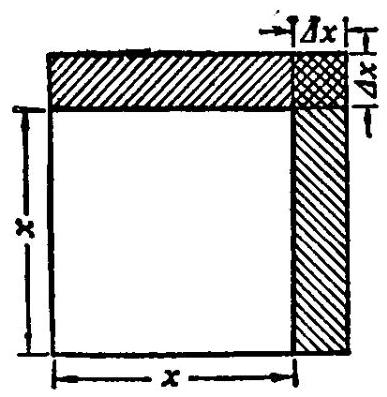
\includegraphics[max width=0.4\textwidth]{images/01912c18-5c3f-733d-b775-749ba9897a9d_110_353714.jpg}
\end{center}

图 2-4

设有边长为 \(x\) 的正方形铁片,加热后边长增加了 \({\Delta x}\) (图 2-4), 求铁片的面积约增加多少.

加热前铁片的面积为 \(y = f\left( x\right) = {x}^{2}\) ,当边长增加了 \({\Delta x}\) ,铁片面积的增加量就是函数 \(f\left( x\right)\) 的改变量

\[
{\Delta y} = {\left( x + \Delta x\right) }^{2} - {x}^{2}
\]

\[
= {x}^{2} + {2x} \cdot {\Delta x} + {\left( \Delta x\right) }^{2} - {x}^{2}
\]

\[
= {2x} \cdot {\Delta x} + {\left( \Delta x\right) }^{2}\text{.} \tag{1}
\]

\({\Delta y}\) 由两部分组成: 一部分是 \({\Delta x}\) 的线性函数 \({2x} \cdot {\Delta x}\) (图 2-4 中单线阴影部分的面积); 另一部分是 \({\left( \Delta x\right) }^{2}\) (图 2-4 中双线阴影部分的面积).

如果以 \({2x} \cdot {\Delta x}\) 作为 \({\Delta y}\) 的近似值,其误差为

\[
{\Delta y} - {2x} \cdot {\Delta x} = {\left( \Delta x\right) }^{2}.
\]

这个误差 \({\left( \Delta x\right) }^{2}\) 显然随着 \(\left| {\Delta x}\right|\) (在这个实际问题中, \({\Delta x} > 0\) ,可以去掉绝对值符号)的减小而减小,而且, \({\left( \Delta x\right) }^{2}\) 要比 \(\left| {\Delta x}\right|\) 减小得更快些 (例如, \(\left| {\Delta x}\right|\) 从 0.1 减小到 0.01, \({\left( \Delta x\right) }^{2}\) 就相应地从 0.01 减小到 0.0001 ),当 \(\left| {\Delta x}\right|\) 很小时, \({\left( \Delta x\right) }^{2}\) 比 \(\left| {\Delta x}\right|\) 要小得多 (例如 \(\left| {\Delta x}\right| = {10}^{-5}\) ,则 \({\left( \Delta x\right) }^{2} = {10}^{-{10}}\) ). 因此式子 \({\Delta y} = {2x} \cdot {\Delta x} + {\left( \Delta x\right) }^{2}\) 右边的两项中,第一项 \({2x} \cdot {\Delta x}\) 是主要部分. 当 \(\left| {\Delta x}\right|\) 很小时,可认为铁片面积增加量

\[
{\Delta y} \approx {2x} \cdot {\Delta x}.
\]

这样我们可以用计算 \({2x\Delta x}\) 来代替计算 \(y = {x}^{2}\) 的改变量 \({\Delta y}\) ,这比计算 \({\Delta y}\) 来得简便,且有一定的精确度.

由 \({2x} = {\left( {x}^{2}\right) }^{\prime } = {f}^{\prime }\left( x\right)\) ,于是在上例中有

\[
{\Delta y} \approx {f}^{\prime }\left( x\right) \cdot {\Delta x}.
\]

\[
\left( {1}^{\prime }\right)
\]

一般地,设函数 \(y = f\left( x\right)\) 在点 \(x\) 处可导,则 \(y = f\left( x\right)\) 在点 \(x\) 处的导数 \({f}^{\prime }\left( x\right)\) 与自变量的改变量 \({\Delta x}\) 的积叫做函数 \(y\) \(= f\left( x\right)\) 在点 \(x\) 处关于改变量 \({\Delta x}\) 的微分,简称函数 \(y\) 的微分, 记作 \({dy}\) ,即

\[
{dy} = {f}^{\prime }\left( x\right) {\Delta x}. \tag{2}
\]

因此,在 \(y = {x}^{2}\) 时,

\[
{\Delta y} \approx {f}^{\prime }\left( x\right) {\Delta x} = {dy}.
\]

\[
\left( {2}^{\prime }\right)
\]

即函数的改变量 \({\Delta y}\) 可用它的微分近似地表示出来. 对于一般的可导函数也有同样的结果, 我们就不证了. 这样, 就可以把计算较为复杂的 \({\Delta y}\) 转化为计算 \({dy}\) ,即只要求出导数值 \({f}^{\prime }\left( x\right)\) 再乘以 \({\Delta x}\) 就行了.

例 半径为 \({10}\mathrm{\;{cm}}\) 的金属圆片加热后,半径伸长了 \({0.05}\mathrm{\;{cm}}\) ,求此时刻面积的微分 \({dA}\) 与 \({\Delta A} - {dA}\) 的值.

解: 以 \(A\) 表示圆片的面积, \(r\) 表示圆片的半径,则

\[
A = \pi {r}^{2}.
\]

根据题意,取 \(r = {10},{\Delta r} = {0.05}\) . 这时,

\[
{dA} = {2\pi r} \cdot {\Delta r}
\]

\[
= {2\pi } \times {10} \times {0.05} = \pi \left( {\mathrm{{cm}}}^{2}\right) \text{.}
\]

\(\because \;{\Delta A} = \pi {\left( r + \Delta r\right) }^{2} - \pi {r}^{2} = {2\pi r} \cdot {\Delta r} + \pi {\left( \Delta r\right) }^{2},\)

\[
\therefore \;{\Delta A} - {dA} = {2\pi r} \cdot {\Delta r} + \pi {\left( \Delta r\right) }^{2} - {2\pi r} \cdot {\Delta r} = \pi {\left( \Delta r\right) }^{2}
\]

\[
= \pi {\left( {0.05}\right) }^{2}
\]

\[
= {0.0025\pi }\left( {\mathrm{{cm}}}^{2}\right) \text{.}
\]

答: 面积的微分 \({dA}\) 为 \(\pi {\mathrm{{cm}}}^{2},{\Delta A} - {dA}\) 为 \({0.0025\pi }{\mathrm{{cm}}}^{2}\) .

在本例中, 如果“加热”改为“冷却”, “伸长”改为“缩短”, 这时,可取 \(r = {10},{\Delta r} = - {0.05}\) ,于是 \({dA}\) 为 \(- \pi {\mathrm{{cm}}}^{2},{\Delta A} - {dA}\) 为 \(- {0.0025\pi }{\mathrm{{cm}}}^{2}\) .

通常把自变量的改变量 \({\Delta x}\) 记作 \({dx}\) ,即 \({dx} = {\Delta x}\) ,称为自变量的微分. 于是函数 \(y = f\left( x\right)\) 的微分也可以写成

\[
{dy} = {f}^{\prime }\left( x\right) {dx}. \tag{3}
\]

在 (3) 式两边同时除以 \({dx}\) ,得到 \({f}^{\prime }\left( x\right) = \frac{dy}{dx}\) . 这样,函数 \(y = f\left( x\right)\) 的导数 \({f}^{\prime }\left( x\right)\) 就等于函数的微分 \({dy}\) 与自变量的微分 \({dx}\) 的商,所以导数也叫做微商. 今后,我们也采用记号 \(\frac{dy}{dx}\) 来表示函数 \(y = f\left( x\right)\) 的导数 \({f}^{\prime }\left( x\right)\) ,即

\[
\frac{dy}{dx} = {f}^{\prime }\left( x\right) = {y}_{x}^{\prime } = \mathop{\lim }\limits_{{{\Delta x} \rightarrow 0}}\frac{\Delta y}{\Delta x}.
\]

我们还采用记号 \(\frac{{d}^{2}y}{d{x}^{2}}\) 来表示二阶导数 \({f}^{\prime \prime }\left( x\right) ,\cdots \cdots\) ,采用记号 \(\frac{{d}^{n}y}{d{x}^{n}}\) 来表示 \(n\) 阶导数 \({f}^{\left( n\right) }\left( x\right)\) 等等.

下面我们来说明函数的微分的几何意义.

设函数 \(y = f\left( x\right)\) 在点 \(x\) 处可导,如图 2-5,在 \(y = f\left( x\right)\) 所表示的曲线上取点 \(P\left( {x,y}\right)\) 及它邻近的点 \({P}^{\prime }\left( {x + {\Delta x},y + {\Delta y}}\right)\) ,过点 \(P\) 及 \({P}^{\prime }\) 作 \({MP}\) 及 \({M}^{\prime }{P}^{\prime }\) 垂直于 \(x\) 轴,分别交 \(x\) 轴于点 \(M\) 及 \({M}^{\prime }\) ,过点 \(P\) 作平行于 \(x\) 轴的直线交 \({M}^{\prime }{P}^{\prime }\) 于点 \(N\) ,又作曲线 \(y = f\left( x\right)\) 在点 \(P\) 处的切线,交 \({M}^{\prime }{P}^{\prime }\) 于点 \(T\) ,则

\[
{PN} = {\Delta x},\;N{P}^{\prime } = {\Delta y},
\]

\[
{NT} = {f}^{\prime }\left( x\right) {\Delta x} = {dy}.
\]

\begin{center}
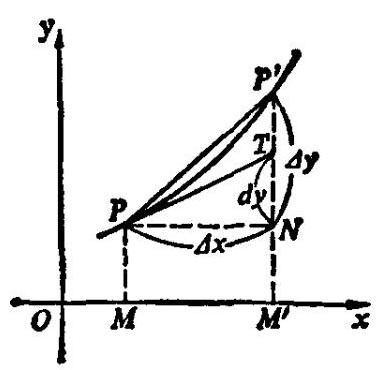
\includegraphics[max width=0.4\textwidth]{images/01912c18-5c3f-733d-b775-749ba9897a9d_113_880246.jpg}
\end{center}

图 2-5

所以,当自变量的改变量为 \({\Delta x}\) 时, \({\Delta y}\) 就是曲线的纵坐标的改变量, \({dy}\) 就是切线的纵坐标的改变量,这就是函数的微分的几何意义. \({\Delta y}\) 与 \({dy}\) 的差的绝对值在图形上是 \(\left| {T{P}^{\prime }}\right|\) ,一般地,它是随着 \(\left| {\Delta x}\right|\) 减小而减小,而且要比 \(\left| {\Delta x}\right|\) 减小得更快些. 所以,当 \(\left| {\Delta x}\right|\) 很小时, \({\Delta y} \approx {dy}\) . 这时,可以用切线的纵坐标的改变量来代替曲线的纵坐标的改变量. 用 \({dy}\) 近似表示 \({\Delta y}\) , 相当于在点 \(P\left( {x,y}\right)\) 附近用切线段 \({PT}\) 近似地代替曲线段 \(P{P}^{\prime }\) . 这种在一定条件下以直代曲的方法是微分和积分中常用的典型方法.

\section{微分的运算}

由微分的表示式 \({dy} = {f}^{\prime }\left( x\right) {dx}\) 知道,已知函数求微分时, 只要求出函数的导数再乘以自变量的微分. 计算微分或导数的方法也叫做微分法.

例 1 求 \(y = \sin x\) 的微分.

\[
\text{解:}\;{dy} = {\left( \sin x\right) }^{\prime }{dx} = \cos {xdx}\text{.}
\]

例 2 求 \(y = \operatorname{arctg}x\) 的微分.

解: \(\;{dy} = {\left( \operatorname{arctg}x\right) }^{\prime }{dx} = \frac{dx}{1 + {x}^{2}}\) .

根据导数的基本公式,利用 \({dy} = {f}^{\prime }\left( x\right) {dx}\) 我们就可求出相应的微分公式.

\section*{微分公式表}

(1) \(d\left( C\right) = 0\) ; (7) \(d\left( {\operatorname{tg}x}\right) = {\sec }^{2}{xdx}\) ;

(2) \(d\left( {x}^{\alpha }\right) = \alpha {x}^{\alpha - 1}{dx}\) ; (8) \(d\left( {\operatorname{ctg}x}\right) = - {\csc }^{2}{xdx}\) ;

(3) \(d\left( {{\log }_{a}x}\right) = \frac{dx}{x\ln a}\) ; (9) \(d\left( {\arcsin x}\right) = \frac{dx}{\sqrt{1 - {x}^{2}}}\) ;

\(d\left( {\ln x}\right) = \frac{dx}{x}\) (10) \(d\left( {\arccos x}\right) = - \frac{dx}{\sqrt{1 - {x}^{2}}}\) ;

(4) \(d\left( {a}^{x}\right) = {a}^{x}\ln {adx}\) ; (11) \(d\left( {\operatorname{arctg}x}\right) = \frac{dx}{1 + {x}^{2}}\) ;

\[
d\left( {e}^{x}\right) = {e}^{x}{dx}
\]

(5) \(d\left( {\sin x}\right) = \cos {xdx}\) ; (12) \(d\left( {\operatorname{arcctg}x}\right) = - \frac{dx}{1 + {x}^{2}}\) .

(6) \(d\left( {\cos x}\right) = - \sin {xdx}\) ;

同样, 由求导数的四则运算法则, 可以得出相应的求微分的四则运算法则:

(1) \(d\left( {u \pm v}\right) = {du} \pm {dv}\) .

(2) \(d\left( {uv}\right) = {udv} + {vdu}\) .

请同学们自己证明(1)、(2)。

(3) \(d\left( \frac{u}{v}\right) = \frac{{vdu} - {udv}}{{v}^{2}}\) .

证明: \(d\left( \frac{u}{v}\right) = {\left( \frac{u}{v}\right) }^{\prime }{dx} = \frac{v{u}^{\prime } - u{v}^{\prime }}{{v}^{2}}{dx}\)

\[
= \frac{v\left( {{u}^{\prime }{dx}}\right) - u\left( {{v}^{\prime }{dx}}\right) }{{v}^{2}} = \frac{{vdu} - {udv}}{{v}^{2}}.
\]

例 3 求 \(y = {e}^{ax}\sin {bx}\) 的微分.

\[
\text{解:}\;{dy} = {e}^{ax}d\left( {\sin {bx}}\right) + \sin {bxd}\left( {e}^{ax}\right)
\]

\[
= {e}^{ax} \cdot b\cos {bxdx} + \sin {bx} \cdot a{e}^{ax}{dx}
\]

\[
= {e}^{ax}\left( {b\cos {bx} + a\sin {bx}}\right) {dx}\text{.}
\]

\begin{problemset}[练习]

\item 对于函数 \(y = {x}^{3} - x\) 和下列的 \({\Delta x}\) 的值,求点 \(x = 2\) 处的 \({\Delta y}\) 和 \({dy}\) :

(1) \({\Delta x} = 1\) ; (2) \({\Delta x} = {0.1}\) ;

(3) \({\Delta x} = {0.01}\) ; (4) \({\Delta x} = {0.001}\) .

\item 求下列函数的微分:

(1) \(y = 3{x}^{4} - 5{x}^{2} + 1\) ; (2) \(y = \left( {2{x}^{2} - 3}\right) \left( {{3x} + 4}\right)\) ;

(3) \(y = \frac{1 - {x}^{2}}{1 + {x}^{2}}\) (4) \(y = \frac{1}{3}{\operatorname{tg}}^{3}\theta + \operatorname{tg}\theta\) ;

(5) \(y = {e}^{2x}\sin {5x}\) ; (6) \(y = \operatorname{arctg}\left( {\ln x}\right)\) .

\item 函数 \(y = f\left( x\right)\) 的微分 \({dy}\) 依赖于哪两个量?

\item 边长 \(4\mathrm{\;{cm}}\) 的正方形铁皮,在加热中边长增加了 \({0.001}\mathrm{\;{cm}}\) , 求此时刻面积的微分 \({dS}\) 与 \({\Delta S} - {dS}\) 的值.

\item 半径 \(R\) 为 \({10}\mathrm{\;{cm}}\) 的球,在冷却中 \(R\) 缩短了 \({0.001}\mathrm{\;{cm}}\) ,求此

时刻体积的微分 \({dV}\) 与 \({\Delta V} - {dV}\) 的值.

\item 求证 \(\frac{d\left( {\sin x}\right) }{d\left( {\cos x}\right) } = - \operatorname{ctg}x\) .

\end{problemset}

\section{近似计算}

我们知道,当 \(\left| {\Delta x}\right|\) 很小时,可以用微分 \({dy}\) 近似代替函数 \(y = f\left( x\right)\) 的改变量 \({\Delta y}\) . 由于在点 \({x}_{0}\) 处,

\[
{dy} = {f}^{\prime }\left( {x}_{0}\right) {\Delta x}
\]

\[
{\Delta y} = f\left( {{x}_{0} + {\Delta x}}\right) - f\left( {x}_{0}\right) ,
\]

于是有

\[
f\left( {{x}_{0} + {\Delta x}}\right) - f\left( {x}_{0}\right) \approx {f}^{\prime }\left( {x}_{0}\right) {\Delta x},
\]

改写一下, 得

\[
f\left( {{x}_{0} + {\Delta x}}\right) \approx f\left( {x}_{0}\right) + {f}^{\prime }\left( {x}_{0}\right) {\Delta x}. \tag{1}
\]

如果把 \({x}_{0} + {\Delta x}\) 记作 \(x\) ,那么 \({\Delta x} = x - {x}_{0}\) ,于是 (1)式也可写成

\[
f\left( x\right) \approx f\left( {x}_{0}\right) + {f}^{\prime }\left( {x}_{0}\right) \left( {x - {x}_{0}}\right) . \tag{2}
\]

如果我们要求函数 \(y = f\left( x\right)\) 在某一点 \(x\) 处的值,但这点的值不易求出,而在 \(x\) 附近的 \({x}_{0}\) 处, \(f\left( {x}_{0}\right)\) 和 \({f}^{\prime }\left( {x}_{0}\right)\) 的值都容易求出,这时,我们可以利用 (2) 式 (或 (1) 式) 来求 \(f\left( x\right)\) 的近似值. 要注意的是这里要求 \(\left| {x - {x}_{0}}\right| = \left| {\Delta x}\right|\) 很小, \(\left| {x - {x}_{0}}\right|\) 越小, 近似程度越好.

例 1 不查表,求 \(\sin {46}^{ \circ }\) 的近似值.

解: 令 \(y = \sin x\) ,由 (2) 式,

\[
\sin x \approx \sin {x}_{0} + \cos {x}_{0} \cdot \left( {x - {x}_{0}}\right) .
\]

因为 \({46}^{ \circ } = {45}^{ \circ } + {1}^{ \circ } = \left( {\frac{\pi }{4} + \frac{\pi }{180}}\right)\) 弧度,

取 \({x}_{0} = \frac{\pi }{4},x = \frac{\pi }{4} + \frac{\pi }{180}\) ,于是 \(x - {x}_{0} = \frac{\pi }{180}\) ,代入上式得

\[
\sin {46}^{ \circ } = \sin \left( {\frac{\pi }{4} + \frac{\pi }{180}}\right)
\]

\[
\approx \sin \frac{\pi }{4} + \cos \frac{\pi }{4} \cdot \frac{\pi }{180}
\]

\[
= \frac{\sqrt{2}}{2} + \frac{\sqrt{2}}{2} \cdot \frac{\pi }{180}
\]

\[
\approx {0.7071} + {0.0123}
\]

\[
= {0.7194}\text{.}
\]

如果把 (2) 式中的 \(x\) 看成变量,(2) 式右边就是 \(x\) 的一次函数. 也就是说,当 \(\left| {x - {x}_{0}}\right|\) 很小时,可以用一次函数 \(y = f\left( {x}_{0}\right)\) \(+ {f}^{\prime }\left( {x}_{0}\right) \left( {x - {x}_{0}}\right)\) 来近似表示函数 \(y = f\left( x\right)\) ; 从几何上看,也就是在点 \(\left( {{x}_{0},{y}_{0}}\right)\) 附近,用曲线 \(y = f\left( x\right)\) 上点 \(\left( {{x}_{0},{y}_{0}}\right)\) 处的切线 \(y - {y}_{0} = {f}^{\prime }\left( {x}_{0}\right) \left( {x - {x}_{0}}\right)\) 来近似表示曲线 \(y = f\left( x\right)\) .

当 \({x}_{0} = 0\) 时,(2)式变为

\[
f\left( x\right) \approx f\left( 0\right) + {f}^{\prime }\left( 0\right) x. \tag{3}
\]

利用(3)式,当 \(\left| x\right|\) 充分小时,可以导出常用的一些近似公式:

\[
\sqrt{1 + x} \approx 1 + \frac{x}{2}
\]

\[
\left( {1}^{ \circ }\right)
\]

\[
\ln \left( {1 + x}\right) \approx x
\]

\[
\left( {2}^{ \circ }\right)
\]

\[
{e}^{x} \approx 1 + x
\]

\[
\left( {3}^{ \circ }\right)
\]

\[
\operatorname{tg}x \approx x\text{.}
\]

\[
\left( {4}^{ \circ }\right)
\]

下面写出这些近似公式的导出过程.

\(\left( {1}^{ \circ }\right)\) 取 \(f\left( x\right) = \sqrt{1 + x}\) ,则

\[
{f}^{\prime }\left( x\right) = \frac{1}{2\sqrt{1 + x}}
\]

于是

\[
f\left( 0\right) = 1,{f}^{\prime }\left( 0\right) = \frac{1}{2}.
\]

由 \(\left( 3\right)\) 式,得

\[
\sqrt{1 + x} = f\left( x\right) \approx f\left( 0\right) + {f}^{\prime }\left( 0\right) x
\]

\[
= 1 + \frac{x}{2}
\]

即

\[
\sqrt{1 + x} \approx 1 + \frac{x}{2}
\]

\(\left( {2}^{ \circ }\right)\) 取 \(f\left( x\right) = \ln \left( {1 + x}\right)\) ,则

\[
{f}^{\prime }\left( x\right) = \frac{1}{1 + x}
\]

于是

\[
f\left( 0\right) = 0,{f}^{\prime }\left( 0\right) = 1\text{. }
\]

由 \(\left( 3\right)\) 式,得

\[
\ln \left( {1 + x}\right) \approx x\text{. }
\]

\begin{itemize}
\item \(\left( {3}^{ \circ }\right)\) 取 \(f\left( x\right) = {e}^{x}\) ,则
\end{itemize}

\[
{f}^{\prime }\left( x\right) = {e}^{x}
\]

于是

\[
f\left( 0\right) = 1,{f}^{\prime }\left( 0\right) = 1\text{. }
\]

由 \(\left( 3\right)\) 式,得

\[
{e}^{x} \approx 1 + x\text{. }
\]

\(\left( {4}^{ \circ }\right)\) 取 \(f\left( x\right) = \operatorname{tg}x\) ,则

\[
{f}^{\prime }\left( x\right) = {\sec }^{2}x
\]

于是

\[
f\left( 0\right) = 0,{f}^{\prime }\left( 0\right) = 1\text{. }
\]

由 \(\left( 3\right)\) 式,得

\[
\operatorname{tg}x \approx x\text{.}
\]

例 2 根据导出的近似公式, 求下列各式的近似值:

(1) \(\sqrt{4.01},\sqrt{8.997}\) ; (2) \(\ln {1.002},\ln {0.998}\) ;

(3) \({e}^{0.01},{e}^{-{0.02}}\) .

解: (1) \(\sqrt{4.01} = \sqrt{4\left( {1 + \frac{0.01}{4}}\right) } = 2\sqrt{1 + \frac{0.01}{4}}\) . 利用公式 \(\left( {1}^{ \circ }\right)\) ,取 \(x = \frac{0.01}{4}\) ,得

\[
\sqrt{4.01} \approx 2\left( {1 + \frac{0.01}{2 \times 4}}\right) = {2.0025}.
\]

\[
\sqrt{8.997} = \sqrt{9\left( {1 - \frac{0.003}{9}}\right) } = 3\sqrt{1 - \frac{0.003}{9}}\text{. 利用公式}\left( {1}^{ \circ }\right) \text{,}
\]

取 \(x = - \frac{0.003}{9}\) ,得

\[
\sqrt{8.997} \approx 3\left( {1 - \frac{0.003}{2 \times 9}}\right) = {2.9995}.
\]

(2)利用公式 \(\left( {2}^{ \circ }\right)\) . 取 \(x = {0.002}\) ,得

\[
\ln {1.002} = \ln \left( {1 + {0.002}}\right) \approx {0.002}\text{.}
\]

取 \(x = - {0.002}\) ,得

\[
\ln {0.998} = \ln \left( {1 - {0.002}}\right) \approx - {0.002}.
\]

(3)利用公式 \(\left( {3}^{ \circ }\right)\) ,取 \(x = {0.01}\) ,得

\[
{e}^{0.01} \approx 1 + {0.01} = {1.01}.
\]

取 \(x = - {0.02}\) ,得

\[
{e}^{-{0.02}} \approx 1 - {0.02} = {0.98}.
\]

例 3 如图 2-6, 加工锥形工件时, 已知工件两头直径分

别为 \({d}_{1},{d}_{2}\) ,长度为 \(l\) ,当斜角 \(\alpha\) 很小时,导出近似关系式:

\[
\alpha \approx {28.6}^{ \circ } \times \frac{{d}_{1} - {d}_{2}}{l}.
\]

\begin{center}
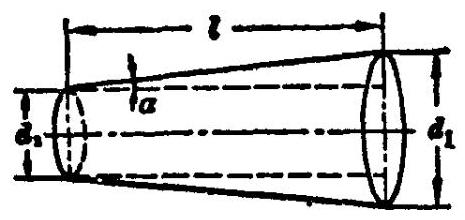
\includegraphics[max width=0.5\textwidth]{images/01912c18-5c3f-733d-b775-749ba9897a9d_120_883650.jpg}
\end{center}

图 2-6

解: 由图,

\[
\operatorname{tg}\alpha = \frac{{d}_{1} - {d}_{2}}{2l}.
\]

当 \(\alpha\) 很小时,根据公式 \(\left( {4}^{ \circ }\right)\) ,

\[
\operatorname{tg}\alpha \approx \alpha ,
\]

\[
\therefore \;\alpha \approx \frac{{d}_{1} - {d}_{2}}{2l}\text{. }
\]

又

\[
\text{1 弧度} = {\left( \frac{180}{\pi }\right) }^{ \circ } \approx {57.3}^{ \circ }\text{,}
\]

\(\therefore \;\alpha \approx {57.3}^{ \circ } \times \frac{{d}_{1} - {d}_{2}}{2l} \approx {28.6}^{ \circ } \times \frac{{d}_{1} - {d}_{2}}{l}\) .

\begin{problemset}[练习]

\item 在例 1 中, \(x - {x}_{0} = \frac{\pi }{180}\) ,是用弧度为单位,为什么? 如果用度为单位,取 \(x - {x}_{0} = 1\) ,得出的结果对不对?

\item 已知 \(\ln {10} = {2.3026}\) ,利用 \(f\left( x\right) \approx f\left( {x}_{0}\right) + {f}^{\prime }\left( {x}_{0}\right) \left( {x - {x}_{0}}\right)\) 求 \(\ln {10.012}\) 的近似值.

\item 当 \(\left| x\right|\) 很小时,导出下列近似公式:

(1) \(\sqrt[n]{1 + x} \approx 1 + \frac{x}{n}\)\(\left( {5}^{ \circ }\right)\)

(2) \(\sin x \approx x\) .\(\left( {6}^{ \circ }\right)\)

\item 计算下列各式的近似值:

(1) \(\sqrt[5]{1.02}\) ; (2) \(\sqrt[3]{0.998}\) ;

(3) \({e}^{-{0.1}}\) (4) \(\operatorname{tg}{0.01}\) ;

(5) \(\sin {0.1}^{ \circ }\) ; (6) \(\ln {1.0021}\) .

\end{problemset}

\begin{problemset}[习 题 八]

\item (1) 在下列图形中,标出相应的 \({\Delta y}\) 和 \({dy}\) 。

\begin{center}
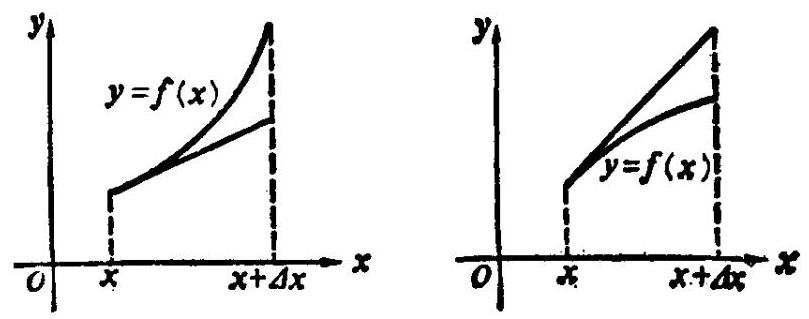
\includegraphics[max width=0.8\textwidth]{images/01912c18-5c3f-733d-b775-749ba9897a9d_121_587843.jpg}
\end{center}

(第 1 (1) 题)

(2)自变量 \(x\) 的微分 \({dx}\) 是否一定为正? 当 \({dx}\) 为正时, 函数 \(y = f\left( x\right)\) 的微分 \({dy}\) 是否一定为正?

\item 求下列函数的微分:

(1) \(y = a{x}^{3} + b{x}^{2} + {cx} + d\) ; (2) \(y = {\left( {a}^{2} - {x}^{2}\right) }^{5}\) ;

(3) \(y = \frac{\left( {x - 1}\right) \left( {x - 2}\right) }{\left( {x + 1}\right) \left( {x + 2}\right) }\) (4) \(r = \left( {1 + {\theta }^{2}}\right) \operatorname{tg}\theta\) ;

(5) \(y = {e}^{-x}\ln x\) ;

(6) \(y = \arcsin {3x} + {3x}\sqrt{1 - 9{x}^{2}}\) ;

(7) \(y = \frac{{x}^{2n}}{{\left( 1 + {x}^{2}\right) }^{n}}\) ; (8) \(y = t - \frac{{e}^{t} - {e}^{-t}}{{e}^{t} + {e}^{-t}}\) .

\item 求函数 \(y = {x}^{3}\) 在自变量的值由 \(x = 1\) 变为 \(x + {\Delta x} = {1.01}\) 时的改变量 \({\Delta y}\) 及 \({dy}\) . 用 \({dy}\) 来近似地代替 \({\Delta y}\) 的误差是多少?

\item 某运动方程为

\[
s = 4{t}^{2}
\]

其中 \(t\) 的单位是秒, \(s\) 的单位是米,求 \(t = 2\) 秒, \({\Delta t} = {0.001}\) 秒时路程的改变量 \({\Delta s}\) 及路程的微分 \({ds}\) ,并加以比较.

\item 一金属圆管的内半径为 \({10}\mathrm{\;{cm}}\) ,厚度为 \({0.05}\mathrm{\;{cm}}\) ,求圆管的横截面积的近似值.

\item 球壳的外直径是 \({30}\mathrm{\;{cm}}\) ,厚度是 \({0.1}\mathrm{\;{cm}}\) ,求球壳体积的近似值.

\item 要在直径为 \({50}\mathrm{\;{cm}}\) 的半球面形锅的内侧镀锌 (锌的比重为 \(7\mathrm{\;g}/{\mathrm{{cm}}}^{3}\) ),镀层厚 \({0.005}\mathrm{\;{cm}}\) ,约需用锌多少克?

\item 计算下列各式的近似值:

(1) \(\sqrt{9.01}\) ; (2) \(\sqrt{15.98}\) ;

(3) \(\sqrt[3]{1.004}\) (4) \(\sqrt[3]{0.982}\) ;

(5) \({e}^{-{0.03}}\) (6) \({\left( {1.002}\right) }^{5}\) ;

(7) \(\ln {1.01}\) ; (8) \(\ln {0.97}\) ;

(9) \(\sin {0.016}\) ; (10) \(\operatorname{tg}{0.025}\) ;

\item 当 \(\left| x\right|\) 很小时,导出近似公式:

\[
{\left( 1 + x\right) }^{\alpha } \approx 1 + {\alpha x}\;\left( {\alpha \text{ 为实数 }}\right) ,
\]

\[
\left( {7}^{ \circ }\right)
\]

并求 \({1.001}^{0.13}\) 的近似值.

\end{problemset}

\chapter*{小 结}
\markboth{小 结}{小 结}

一、本章主要内容是导数和微分的概念、求导数和求微分的方法以及微分在近似计算上的某些应用.

二、导数概念是微积分学的基本概念之一. 函数 \(y = f\left( x\right)\)

的导数 \({f}^{\prime }\left( x\right)\) ,就是函数的改变量 \({\Delta y}\) 与自变量的改变量 \({\Delta x}\) 的比 \(\frac{\Delta y}{\Delta x}\) 当 \({\Delta x} \rightarrow 0\) 时的极限,即

\[
{f}^{\prime }\left( x\right) = \mathop{\lim }\limits_{{{\Delta x} \rightarrow 0}}\frac{\Delta y}{\Delta x} = \mathop{\lim }\limits_{{{\Delta x} \rightarrow 0}}\frac{f\left( {x + {\Delta x}}\right) - f\left( x\right) }{\Delta x},
\]

它表示在点 \(x\) 处函数 \(y\) 对自变量的变化率,它的几何意义是曲线 \(y = f\left( x\right)\) 在点 \(\left( {x,f\left( x\right) }\right)\) 处的切线的斜率.

如果 \({f}^{\prime }\left( {x}_{0}\right)\) 存在,曲线 \(y = f\left( x\right)\) 上点 \(\left( {{x}_{0},{y}_{0}}\right)\) 处的切线的方程为

\[
y - {y}_{0} = {f}^{\prime }\left( {x}_{0}\right) \left( {x - {x}_{0}}\right)
\]

法线的方程 (当 \({f}^{\prime }\left( {x}_{0}\right) \neq 0\) 时) 为

\[
y - {y}_{0} = - \frac{1}{{f}^{\prime }\left( {x}_{0}\right) }\left( {x - {x}_{0}}\right) .
\]

三、函数 \(y = f\left( x\right)\) 的微分 \({dy}\) 就是函数的导数 \({f}^{\prime }\left( x\right)\) 与自变量的微分 \({dx}\left( {{dx} = {\Delta x} \neq 0}\right)\) 的积,即

\[
{dy} = {f}^{\prime }\left( x\right) {dx}.
\]

求函数 \(y = f\left( x\right)\) 的导数 \({f}^{\prime }\left( x\right)\) 与求函数的微分 \({f}^{\prime }\left( x\right) {dx}\) 是互通的, 即

\[
\frac{dy}{dx} = {f}^{\prime }\left( x\right) \Leftrightarrow {dy} = {f}^{\prime }\left( x\right) {dx},
\]

所以导数也叫做微商.

四、求函数的导数或微分的方法叫做微分法. 根据定义求导数是最基本的方法. 对初等函数来说, 只要根据定义先求得一些基本初等函数的导数, 再利用求导数 (或微分) 的四则运算法则以及复合函数、反函数的求导 (或微分) 法则, 就可以求出任一初等函数的导数 (或微分). 这里, 复合函数的求导法则特别重要, 应切实掌握.

五、根据微分的定义及其几何意义, 有下列近似公式:

\[
{\Delta y} \approx {f}^{\prime }\left( {x}_{0}\right) {\Delta x}\;\left( {\left| {\Delta x}\right| \text{ 很小 }}\right) ,
\]

\[
f\left( x\right) \approx f\left( {x}_{0}\right) + {f}^{\prime }\left( {x}_{0}\right) \left( {x - {x}_{0}}\right) \;\left( {\left| {x - {x}_{0}}\right| \text{ 很小 }}\right) .
\]

利用这些公式, 可以求出函数的改变量或在某一点处的函数值的近似值.

特别当 \({x}_{0} = 0\) 时,有

\[
f\left( x\right) \approx f\left( 0\right) + {f}^{\prime }\left( 0\right) x\;\left( {\left| x\right| \text{ 很小 }}\right) .
\]

由此可以导出一些常用的近似公式, 从而使实际问题中的一些计算大为简化.

\chapter*{复习参考题二}
\markboth{复习参考题二}{复习参考题二}

\section*{\(A\) 组}

1. (1) 在导数的定义中, \(\mathop{\lim }\limits_{{{\Delta x} \rightarrow 0}}\frac{\Delta y}{\Delta x}\) 的 \({\Delta x}\) 是正的还是负的? 还

是可正可负? \(\mathop{\lim }\limits_{{{\Delta x} \rightarrow 0 + }}\frac{\Delta y}{\Delta x}\) 的 \({\Delta x}\) 呢? \(\mathop{\lim }\limits_{{{\Delta x} \rightarrow 0}}\frac{\Delta y}{\Delta x}\) 的 \({\Delta x}\) 呢?

\(\mathop{\lim }\limits_{{{\Delta x} \rightarrow 0}}\frac{\Delta y}{\Delta x}\) 与 \(\mathop{\lim }\limits_{{{\Delta x} \rightarrow 0 + }}\frac{\Delta y}{\Delta x}\) 及 \(\mathop{\lim }\limits_{{{\Delta x} \rightarrow 0 - }}\frac{\Delta y}{\Delta x}\) 之间有什么关系?

(2) \({f}^{\prime }\left( x\right)\) 和 \({f}^{\prime }\left( {x}_{0}\right)\) 有什么不同? \({f}^{\prime }\left( {x}_{0}\right)\) 与 \({\left\lbrack f\left( {x}_{0}\right) \right\rbrack }^{\prime }\) 有什么不同?

2. 一质点沿 \({OA}\) 轴运动,在时刻 \(t\) (秒)时,质点的位置 \(s = {6t} - {t}^{2}\) (米).

(1)求 \(t = 0,2,3,6,7\) 时质点的位置. 当 8 取负值时意

味着什么?

(2)求速度 \(v\left( {\text{米}/\text{秒}}\right)\) 的表示式,并求 \(t = 0,2,3,6,7\) 时的 \(v\) 值. \(v\) 值为负时意味着什么?

(3)什么时刻以后, 质点改变运动的方向?

3. 在受到制动后的 \(t\) 秒钟内飞轮转过的角度(弧度)由函数 \(\varphi \left( t\right) = {4t} - {0.3}{t}^{2}\) 给出,求:

(1) \(t = 2\) (秒) 时,飞轮转过的角度;

(2)飞轮停止旋转的时刻.

4. 假设 1 公斤的铁从 \({0}^{ \circ }\mathrm{C}\) 加热到 \({t}^{ \circ }\mathrm{C}\left( {0 \leq t \leq {200}}\right)\) 时,所吸收的热量 \(Q\left( \text{千卡 }\right)\) 由公式 \(Q\left( t\right) = {0.1053t} + {0.000071}{t}^{2}\) 确定,求 \(t = {50}\) 时铁的比热 \(C\) .

(提示: 比热 \(C = {Q}^{\prime }\left( t\right)\) 千卡/公斤. 度. )

5. 已知抛物线 \(y = {x}^{2} - 4\) 及直线 \(y = x + 2\) ,求直线与抛物线在交点处的切线的交角.

6. 已知两曲线 \(y = {x}^{2} - 1\) 与 \(y = 1 - {x}^{3}\) .

(1)这两曲线在横坐标为 \({x}_{0}\) 的点处的切线互相平行,求 \({x}_{0}\) 的值;

(2)这两曲线在横坐标为 \({x}_{1}\) 的点处的切线互相垂直,求 \({x}_{1}\) 的值.

7. 按定义求 \(y = \operatorname{tg}x\) 的导数.

8. 求下列函数的导数:

(1) \(y = \left( {{x}^{2} - 1}\right) \left( {{x}^{2} - 3}\right) \left( {{x}^{2} - 5}\right)\) ; (2) \(y = \frac{{x}^{2}}{{\left( {x}^{2} - 1\right) }^{3}}\) ;

(3) \(y = \frac{\sin {2x}}{1 + x}\) (4) \(y = \frac{\sec x}{1 + \operatorname{tg}x}\)

(5) \(y = {\sin }^{4}{3x}{\cos }^{3}{4x}\) ; (6) \(y = 2\left( {{e}^{\frac{x}{2}} + {e}^{-\frac{x}{2}}}\right)\) ;

(7) \(y = x\arcsin \frac{x}{2} + \sqrt{4 - {x}^{2}}\) ; (8) \(y = {a}^{{2x} + 1}\) ;

(9) \(y = \arccos \frac{x - 3}{3} - 2\sqrt{\frac{6 - x}{x}}\)

(10) \(y = \frac{x\ln x}{x + 1} - \ln \left( {x + 1}\right)\) ; (11) \(y = \lg \left( {{x}^{2} + x + 1}\right)\) ;

(12) \(y = \ln \left( {{\cos }^{2}x}\right) + {2x}\operatorname{tg}x - {x}^{2}\) .

9. 求下列函数的导数:

(1) \(y = \frac{x - a}{\sqrt{{x}^{2} - {2ax}}}\) ; (2) \(y = \operatorname{arctg}\frac{x - a}{x + a}\)

(3) \(y = \frac{x}{2}\sqrt{{x}^{2} + {a}^{2}} + \frac{{a}^{2}}{2}\ln \frac{x + \sqrt{{x}^{2} + {a}^{2}}}{a}\) ;

(4) \(y = \operatorname{arctg}\left( {\sec x + \operatorname{tg}x}\right)\) ;

(5) \(y = \ln \left( {\ln x}\right) - \frac{1}{\ln x}\) ; (6) \(y = \ln \left( {\operatorname{tg}\left( {\frac{\pi }{4} - \frac{x}{2}}\right) }\right)\) ;

(7) \(y = {e}^{\arcsin \sqrt{x}}\) ; (8) \(y = \lg \left( {{a}^{x} + {b}^{x}}\right)\) ;

(9) \(y = {a}^{\operatorname{tg}x}\) ;

(10) \(y = \arcsin \frac{2}{{e}^{x} + {e}^{-x}}\left( {x > 0}\right)\) ;

(11) \(y = \sqrt{\left( {x - a}\right) \left( {x - b}\right) \left( {x - c}\right) }\) ;

(12) \(y = \ln \left( {\csc x - \operatorname{ctg}x}\right)\) .

10. 一金属圆盘受热膨胀, 它的半径以 0.01 厘米/秒 的速度均匀增大, 当它的半径等于 2 厘米时, 它的面积的增大速度是多少?

(提示: 圆面积 \(S = \pi {r}^{2}\) ,把 \(S\) 和 \(r\) 都看成 \(t\) 的函数.)

11. 求证抛物线 \(\sqrt{x} + \sqrt{y} = \sqrt{a}\) 上任意一点处的切线在两坐标轴上截距的和等于 \(a\) .

12. 求垂直于直线 \({2x} + {4y} - 3 = 0\) 并与双曲线 \(\frac{{x}^{2}}{2} - \frac{{y}^{2}}{7} = 1\) 相切的直线的方程。

13. 某运动物体由点 \(O\) 开始作直线运动,经过 \(t\) 秒后它和点 \(O\) 的距离为

\[
s = \frac{1}{4}{t}^{4} - 4{t}^{3} + {16}{t}^{2}
\]

(1)此物体什么时刻在 \(O\) 点 \(\left( {\text{即}s = 0}\right)\) ?

(2)什么时刻它的速度为 0 ?

(3)什么时刻它的加速度值为 11 ?

14. 求下列函数的二阶导数:

(1) \(y = \sin {ax} + \cos {bx}\) ; (2) \(y = {e}^{\sqrt{x}} + {e}^{-\sqrt{x}}\)

(3) \(y = \frac{{x}^{2} + 1}{{\left( x + 1\right) }^{3}}\) (4) \(y = \operatorname{arctg}\frac{{e}^{x} - {e}^{-x}}{2}\) .

15. 求下列函数 \(y\) 在指定点处的一阶导数及二阶导数:

(1) \(y = \sqrt{3x} + \frac{13}{\sqrt{3x}}\) ,点 \(x = 3\) ;

(2) \(y = x\sqrt{{x}^{2} - {16}}\) ,点 \(x = 5\) .

16. 一物体作阻尼运动, 运动规律为

\[
x = {e}^{-{2t}}\sin \left( {{3t} + \frac{\pi }{6}}\right)
\]

求运动物体的速度和加速度。

17. 求下列函数的微分:

(1) \(y = {\left( 2{x}^{3} - 3{x}^{2} + 6x\right) }^{2}\) ;

(2) \(y = {\left( {e}^{x} + {e}^{-x}\right) }^{2}\) ; (3) \(y = \frac{\ln x}{\sqrt{x}}\)

(4) \(y = \operatorname{arctg}\frac{1 - {x}^{2}}{1 + {x}^{2}}\) .

18. 设 \(y = {\cos }^{2}\varphi\) ,当 \(\varphi\) 从 \({60}^{ \circ }\) 变到 \({60}^{ \circ }{30}^{\prime }\) 时,求函数 \(y\) 的微分.

19. 单摆的周期 \(T\) (秒) 与单摆的长度 \(l\) (厘米)之间,有关系 \(T = {2\pi }\sqrt{\frac{l}{980}}\) . 长度为 20 厘米的单摆加长 1 厘米后,它的周期大约增加多少?

20. 利用近似公式 \(f\left( x\right) \approx f\left( {x}_{0}\right) + {f}^{\prime }\left( {x}_{0}\right) \left( {x - {x}_{0}}\right)\) 求下列各式的近似值:

(1) \(\sin {29}^{ \circ }\) ; (2) \(\operatorname{arctg}{0.97}\) .

21. 当 \(\left| x\right|\) 很小时,导出下列近似公式:

(1) \(\frac{1}{1 + x} \approx 1 - x\) ;\(\left( {8}^{ \circ }\right)\)

(2) \(\operatorname{arctg}x \approx x\) .\(\left( {9}^{ \circ }\right)\)

22. 计算下列各式的近似值:

(1) \(\sqrt[8]{1.02}\) ; (2) \(\frac{1}{\sqrt{99.5}}\) (3) \({\log }_{1.01}{0.997}\) .

23. 已知 \(f\left( x\right) = \frac{x}{\sqrt{{x}^{2} + 9}}\) ,求 \(f\left( {0.03}\right)\) 的近似值.

\begin{center}
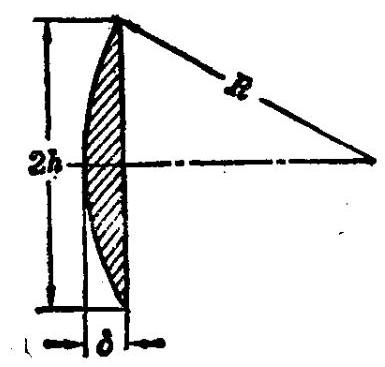
\includegraphics[max width=0.4\textwidth]{images/01912c18-5c3f-733d-b775-749ba9897a9d_128_440234.jpg}
\end{center}

(第 24 题)

24. 如图,一透镜的凸面半径是 \(R\) , 四径是 \({2h}\) ( \(h\) 比 \(R\) 小得多),厚度是 \(\delta\) . 导出近似关系式:

\[
\delta \approx \frac{{h}^{2}}{2R}
\]

\section*{\(B\) 组}

25. 证明双曲线 \({xy} = a(a\) 为不等于零的常数) 上任意一点处的切线和坐标轴所构成的三角形的面积等于 \(2\left| a\right|\) .

26. 设函数

\[
f\left( x\right) = \left\{ \begin{array}{ll} {x}^{2}, & x \leq 1; \\ {ax} + b, & x > 1. \end{array}\right.
\]

为了使 \(f\left( x\right)\) 在点 \(x = 1\) 处连续而且可导,应该怎样选取系数 \(a,b\) ?

27. 把 \(y = \arcsin x\) 变形为 \(x = \sin y\) ,利用隐函数的求导法则, 证明:

\[
{\left( \arcsin x\right) }^{\prime } = \frac{1}{\sqrt{1 - {x}^{2}}}
\]

\begin{center}
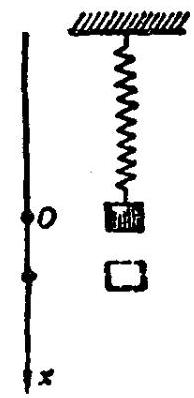
\includegraphics[max width=0.2\textwidth]{images/01912c18-5c3f-733d-b775-749ba9897a9d_129_320008.jpg}
\end{center}

(第 28 题)

28. 一质量为 3 公斤的物体挂于弹簧的下端,在 \(O\) 点上下振动,振动规律为 \(x = {10}\sin t\) . 求振动过程中的最大动能.

(位移单位为厘米, 时间单位为秒.)

29. 一倒置圆锥形的容器, 它的轴截面是一等边三角形. 以每秒 100 立方厘米的速度往容器内加水, 求当水面高度为 20 厘米时水面上升的速度. (提示: 先写出容器内水的体积与水面高度的函数关系.)

30. 从上口直径为 12 厘米, 深为 18 厘米的锥形漏斗中流出溶液, 当液面高度从 10 厘米下降到 9.8 厘米时, 求流出溶液的容积的近似值。


\subsection{在线使用模板}

我们把三套模板全部上传到 \href{https://www.overleaf.com/}{Overleaf} 上了,网络便利的用户可以直接通过 Overleaf 在线使用我们的模板。使用 Overleaf 的好处是无需安装 \TeX{} Live,可以随时随地访问自己的文件。查找模板,请在 Overleaf 模板库里面搜索 \lstinline{elegantlatex} 即可,你也可以直接访问\href{https://www.overleaf.com/latex/templates?addsearch=elegantlatex}{搜索结果}。选择适当的模板之后,将其 \lstinline{Open as Template},即可把模板存到自己账户下,然后可以自由编辑以及与别人一起协作。更多关于 Overleaf 的介绍和使用,请参考 Overleaf 的\href{https://www.overleaf.com/learn}{官方文档}。

\subsection{本地免安装使用}

\textbf{免安装}使用方法如下:从 GitHub 或者 CTAN 下载最新版,严格意义上只需要类文件 \lstinline{elegantbook.cls}。然后将模板文件放在你的工作目录下即可使用。这样使用的好处是,无需安装,简便;缺点是,当模板更新之后,你需要手动替换 \lstinline{cls} 文件。

\subsection{发行版安装与更新}

本模板测试环境为 
\begin{enumerate}
	\item Win10 + \TeX{} Live 2022;
	\item Ubuntu 20.04 + \TeX{} Live 2022;
	\item macOS Monterey + Mac\TeX{} 2022。
\end{enumerate}

\TeX Live/Mac\TeX{} 的安装请参考啸行的\href{https://github.com/OsbertWang/install-latex-guide-zh-cn/releases/}{一份简短的关于安装 \LaTeX{} 安装的介绍}。

安装 \TeX{} Live 之后,安装后建议升级全部宏包,升级方法:使用 cmd 或 terminal 运行 \lstinline{tlmgr update --all},如果 tlmgr 需要更新,请使用 cmd 运行 \lstinline{tlmgr update --self},如果更新过程中出现了中断,请改用 \lstinline{tlmgr update --self --all --reinstall-forcibly-removed} 更新,也即

\begin{lstlisting}
	tlmgr update --self 
	tlmgr update --all
	tlmgr update --self --all --reinstall-forcibly-removed
\end{lstlisting}

更多的内容请参考 \href{https://tex.stackexchange.com/questions/55437/how-do-i-update-my-tex-distribution}{How do I update my \TeX{} distribution?}

\subsection{其他发行版本}

由于宏包版本问题,本模板不支持 C\TeX{} 套装,请务必安装 TeX Live/Mac\TeX{}。更多关于 \TeX{} Live 的安装使用以及 C\TeX{} 与 \TeX{} Live 的兼容、系统路径问题,请参考官方文档以及啸行的\href{https://github.com/OsbertWang/install-latex-guide-zh-cn/releases/}{一份简短的关于安装 \LaTeX{} 安装的介绍}。



\chapter{Elegant\LaTeX{} 系列模板介绍}

\begin{quotation}
  \textbf{\textcolor{red}{本模板自 2023 年 1 月 1 日开始,不再维护,不建议使用本系列模板!为了保证之前版本的用户仍然能查到说明文档,本说明文档仍然保留过去的信息。}}
\end{quotation}

Elegant\LaTeX{} 项目组致力于打造一系列美观、优雅、简便的模板方便用户使用。目前由 \href{https://github.com/ElegantLaTeX/ElegantNote}{ElegantNote},\href{https://github.com/ElegantLaTeX/ElegantBook}{ElegantBook},\href{https://github.com/ElegantLaTeX/ElegantPaper}{ElegantPaper} 组成,分别用于排版笔记,书籍和工作论文。大版本改动较大,请关注版本信息,在未开始使用模板前,建议直接选择最新正式版本!


本文将介绍本模板的一些设置内容以及基本使用方法。如果您有其他问题,建议或者意见,欢迎在 GitHub 上给我们提交 \href{https://github.com/ElegantLaTeX/ElegantBook/issues}{issues} 或者邮件联系我们。我们的联系方式如下,建议加入用户 QQ 群提问,这样能更快获得准确的反馈,加群时请备注 \LaTeX{} 或者 Elegant\LaTeX{} 相关内容。
\begin{itemize}
  \item 官网:\href{https://elegantlatex.org/}{https://elegantlatex.org/}
  \item GitHub 地址:\href{https://github.com/ElegantLaTeX/}{https://github.com/ElegantLaTeX/}
  \item CTAN 地址:\href{https://ctan.org/pkg/elegantbook}{https://ctan.org/pkg/elegantbook}
  \item 下载地址:\href{https://github.com/ElegantLaTeX/ElegantBook/releases}{正式发行版},\href{https://github.com/ElegantLaTeX/ElegantBook/archive/master.zip}{最新版}
  \item Bilibili:\href{https://space.bilibili.com/516479629}{ElegantLaTeX}
  \item 用户 QQ 群:692108391
\end{itemize}


\section{模板安装与更新}

你可以通过免安装的方式使用本模板,包括在线使用和本地(文件夹内)使用两种方式,也可以通过 \TeX{} 发行版安装使用。

\subsection{在线使用模板}

我们把三套模板全部上传到 \href{https://www.overleaf.com/}{Overleaf} 上了,网络便利的用户可以直接通过 Overleaf 在线使用我们的模板。使用 Overleaf 的好处是无需安装 \TeX{} Live,可以随时随地访问自己的文件。查找模板,请在 Overleaf 模板库里面搜索 \lstinline{elegantlatex} 即可,你也可以直接访问\href{https://www.overleaf.com/latex/templates?addsearch=elegantlatex}{搜索结果}。选择适当的模板之后,将其 \lstinline{Open as Template},即可把模板存到自己账户下,然后可以自由编辑以及与别人一起协作。更多关于 Overleaf 的介绍和使用,请参考 Overleaf 的\href{https://www.overleaf.com/learn}{官方文档}。

\subsection{本地免安装使用}

\textbf{免安装}使用方法如下:从 GitHub 或者 CTAN 下载最新版,严格意义上只需要类文件 \lstinline{elegantbook.cls}。然后将模板文件放在你的工作目录下即可使用。这样使用的好处是,无需安装,简便;缺点是,当模板更新之后,你需要手动替换 \lstinline{cls} 文件。

\subsection{发行版安装与更新}

本模板测试环境为 
\begin{enumerate}
  \item Win10 + \TeX{} Live 2022;
  \item Ubuntu 20.04 + \TeX{} Live 2022;
  \item macOS Monterey + Mac\TeX{} 2022。
\end{enumerate}

\TeX Live/Mac\TeX{} 的安装请参考啸行的\href{https://github.com/OsbertWang/install-latex-guide-zh-cn/releases/}{一份简短的关于安装 \LaTeX{} 安装的介绍}。

安装 \TeX{} Live 之后,安装后建议升级全部宏包,升级方法:使用 cmd 或 terminal 运行 \lstinline{tlmgr update --all},如果 tlmgr 需要更新,请使用 cmd 运行 \lstinline{tlmgr update --self},如果更新过程中出现了中断,请改用 \lstinline{tlmgr update --self --all --reinstall-forcibly-removed} 更新,也即

\begin{lstlisting}
tlmgr update --self 
tlmgr update --all
tlmgr update --self --all --reinstall-forcibly-removed
\end{lstlisting}

更多的内容请参考 \href{https://tex.stackexchange.com/questions/55437/how-do-i-update-my-tex-distribution}{How do I update my \TeX{} distribution?}

\subsection{其他发行版本}

由于宏包版本问题,本模板不支持 C\TeX{} 套装,请务必安装 TeX Live/Mac\TeX{}。更多关于 \TeX{} Live 的安装使用以及 C\TeX{} 与 \TeX{} Live 的兼容、系统路径问题,请参考官方文档以及啸行的\href{https://github.com/OsbertWang/install-latex-guide-zh-cn/releases/}{一份简短的关于安装 \LaTeX{} 安装的介绍}。



\chapter{ElegantBook 设置说明}

本模板基于基础的 book 文类,所以 book 的选项对于本模板也是有效的(纸张无效,因为模板有设备选项)。默认编码为 UTF-8,推荐使用 \TeX{} Live 编译。

\section{语言模式}
本模板内含两套基础语言环境 \lstinline{lang=cn}、\lstinline{lang=en}。改变语言环境会改变图表标题的引导词(图,表),文章结构词(比如目录,参考文献等),以及定理环境中的引导词(比如定理,引理等)。不同语言模式的启用如下:
\begin{lstlisting}
\documentclass[cn]{elegantbook} 
\documentclass[lang=cn]{elegantbook}
\end{lstlisting}

除模板自带的两套语言设定之外,由\textbf{网友}提供的其他语言环境设置如下:
\begin{itemize}
  \item 由 \href{https://github.com/VincentMVV}{VincentMVV} 提供的意大利语翻译 \lstinline{lang=it},相关讨论见 \href{https://github.com/ElegantLaTeX/ElegantBook/issues/85}{Italian translation};
  \item 由 \href{https://github.com/abfek66}{abfek66} 提供的法语翻译 \lstinline{lang=fr},相关讨论见 \href{https://github.com/ElegantLaTeX/ElegantBook/issues/85}{Italian translation};
  % \item 由 \href{https://github.com/stultus}{stultus} 提供的马拉雅拉姆语翻译 \lstinline{lang=},相关讨论见 \href{https://github.com/ElegantLaTeX/ElegantBook/issues/90}{Malayalam translation};
  \item 由 \href{https://github.com/inktvis75}{inktvis75} 提供的荷兰语翻译 \lstinline{lang=nl},相关讨论见 \href{https://github.com/ElegantLaTeX/ElegantBook/issues/108}{Dutch Translation};
  \item 由 \href{https://github.com/palkotamas}{palkotamas} 提供的匈牙利语翻译 \lstinline{lang=hu},相关讨论见 \href{https://github.com/ElegantLaTeX/ElegantBook/issues/111}{Hungarian translation};
  \item 由 Lisa 提供的德语翻译 \lstinline{lang=de},相关讨论见 \href{https://github.com/ElegantLaTeX/ElegantBook/issues/113}{Deutsch translation};
  \item 由 Gustavo A. Corradi 提供的西班牙语的翻译 \lstinline{lang=es},相关讨论见 \href{https://github.com/ElegantLaTeX/ElegantBook/issues/133}{Spanish translation};
  \item 由 \href{https://github.com/Altantsooj}{Altantsooj} 提供的蒙古语的翻译 \lstinline{lang=mn},相关讨论见 \href{https://github.com/ElegantLaTeX/ElegantBook/issues/137}{Mongolian translation};
  \item 由 \href{https://github.com/inusturbo}{inusturbo} 提供的日本语的翻译 \lstinline{lang=jp},相关讨论见 \href{https://github.com/ElegantLaTeX/ElegantBook/issues/172}{Japanese Translation}。
\end{itemize}



\begin{remark}
以上各个语言的设定均为网友设定,我们未对上述翻译进行过校对,如果有问题,请在对应的 issue 下评论。并且,只有中文环境(\lstinline{lang=cn})才可以输入中文。
\end{remark}

\section{设备选项}
最早我们在 ElegantNote 模板中加入了设备选项(\lstinline{device}),后来,我们觉得这个设备选项的设置可以应用到 ElegantBook 中\footnote{不过因为 ElegantBook 模板封面图片的存在,在修改页面设计时,需要对图片进行裁剪。},而且 Book 一般内容比较多,如果在 iPad 上看无需切边,放大,那用户的阅读体验将会得到巨大提升。你可以使用下面的选项将版面设置为 iPad 设备模式\footnote{默认为 normal 模式,也即 A4 纸张大小。}
\begin{lstlisting}
\documentclass[pad]{elegantbook} %or
\documentclass[device=pad]{elegantbook}
\end{lstlisting}

\section{颜色主题}

本模板内置 5 组颜色主题,分别为 \textcolor{structure1}{\lstinline{green}}\footnote{为原先默认主题。}、\textcolor{structure2}{\lstinline{cyan}}、\textcolor{structure3}{\lstinline{blue}}(默认)、\textcolor{structure4}{\lstinline{gray}}、\textcolor{structure5}{\lstinline{black}}。另外还有一个自定义的选项  \lstinline{nocolor}。调用颜色主题 \lstinline{green} 的方法为 
\begin{lstlisting}
\documentclass[green]{elegantbook} %or
\documentclass[color=green]{elegantbook}
\end{lstlisting}


\begin{table}[htbp]
  \caption{ElegantBook 模板中的颜色主题\label{tab:color thm}}
  \centering
  \begin{tabular}{ccccccc}
  \toprule
    & \textcolor{structure1}{green} 
    & \textcolor{structure2}{cyan} 
    & \textcolor{structure3}{blue}
    & \textcolor{structure4}{gray} 
    & \textcolor{structure5}{black} 
    & 主要使用的环境\\
  \midrule
    structure & \ccr{structure1}
    & \ccr{structure2}
    & \ccr{structure3} 
    & \ccr{structure4} 
    & \ccr{structure5} 
    & chapter \ section \ subsection \\
    main      & \ccr{main1}
    & \ccr{main2}
    & \ccr{main3}
    & \ccr{main4}
    & \ccr{main5}
    & definition \ exercise \ problem \\
    second    & \ccr{second1}
    & \ccr{second2}
    & \ccr{second3}
    & \ccr{second4}
    & \ccr{second5}
    & theorem \ lemma \ corollary\\
    third     & \ccr{third1}
    & \ccr{third2}
    & \ccr{third3}
    & \ccr{third4}
    & \ccr{third5}
    & proposition\\
  \bottomrule
  \end{tabular}
\end{table}

如果需要自定义颜色的话请选择 \lstinline{nocolor} 选项或者使用 \lstinline{color=none},然后在导言区定义 structurecolor、main、second、third 颜色,具体方法如下:
\begin{lstlisting}[tabsize=4]
\definecolor{structurecolor}{RGB}{0,0,0}
\definecolor{main}{RGB}{70,70,70}    
\definecolor{second}{RGB}{115,45,2}    
\definecolor{third}{RGB}{0,80,80}
\end{lstlisting}

\section{封面}

\subsection{封面个性化}

从 3.10 版本开始,封面更加弹性化,用户可以自行选择输出的内容,包括 \lstinline{\title} 在内的所有封面元素都可为空。目前封面的元素有

\begin{table}[htbp]
  \centering
  \caption{封面元素信息}
  \begin{tabular}{p{0.07\textwidth}p{0.15\textwidth}|p{0.07\textwidth}p{0.15\textwidth}|p{0.07\textwidth}p{0.15\textwidth}}
    \hline
    信息 & 命令 & 信息 & 命令 & 信息 & 命令 \\
    \hline
    标题 & \lstinline|\title| & 副标题 & \lstinline|\subtitle| & 作者 & \lstinline|\author| \\
    机构 & \lstinline|\institute| & 日期 &  \lstinline|\date| & 版本 & \lstinline|\version| \\
    箴言 & \lstinline|\extrainfo| & 封面图 & \lstinline|\cover| & 徽标 & \lstinline|\logo| \\
    \hline
  \end{tabular}
\end{table}

另外,额外增加一个 \lstinline{\bioinfo} 命令,有两个选项,分别是信息标题以及信息内容。比如需要显示{\kaishu User Name:111520},则可以使用 
\begin{lstlisting}
\bioinfo{User Name}{115520}
\end{lstlisting}

封面中间位置的色块的颜色可以使用下面命令进行修改:
\begin{lstlisting}
\definecolor{customcolor}{RGB}{32,178,170}
\colorlet{coverlinecolor}{customcolor}
\end{lstlisting}

\subsection{封面图}

本模板使用的封面图片来源于 \href{https://pixabay.com/en/tea-time-poetry-coffee-reading-3240766/}{pixabay.com}\footnote{感谢 China\TeX{} 提供免费图源网站,另外还推荐 \href{https://www.pexels.com/}{pexels.com}。},图片完全免费,可用于任何场景。封面图片的尺寸为 $1280 \times 1024$, 更换图片的时候请\textbf{严格}按照封面图片尺寸进行裁剪。推荐一个免费的在线图片裁剪网站 \href{https://www.fotor.com/cn}{fotor.com}。用户 QQ 群内有一些合适尺寸的封面,欢迎取用。

\subsection{徽标}

本文用到的 Logo 比例为 1:1,也即正方形图片,在更换图片的时候请选择合适的图片进行替换。

\subsection{自定义封面}

另外,如果使用自定义的封面,比如 Adobe illustrator 或者其他软件制作的 A4 PDF 文档,请把 \lstinline{\maketitle} 注释掉,然后借助 \lstinline{pdfpages} 宏包将自制封面插入即可。如果使用 \lstinline{titlepage} 环境,也是类似。如果需要 2.x 版本的封面,请参考 \href{https://github.com/EthanDeng/etitlepage}{etitlepage}。

\section{章标标题}

本模板内置 2 套\textit{章标题显示风格},包含 \lstinline{hang}(默认)与 \lstinline{display} 两种风格,区别在于章标题单行显示(\lstinline{hang})与双行显示(\lstinline{display}),本说明使用了 \lstinline{hang}。调用方式为
\begin{lstlisting}
\documentclass[hang]{elegantbook} %or
\documentclass[titlestyle=hang]{elegantbook}
\end{lstlisting}

在章标题内,章节编号默认是以数字显示,也即{\kaishu 第 1 章},{\kaishu 第 2 章}等等,如果想要把数字改为中文,可以使用
\begin{lstlisting}
\documentclass[chinese]{elegantbook} %or
\documentclass[scheme=chinese]{elegantbook}
\end{lstlisting}

\section{数学环境简介}

在我们这个模板中,我们定义了两种不同的定理模式 \lstinline{mode},包括简单模式(\lstinline{simple})和炫彩模式(\lstinline{fancy}),默认为 \lstinline{fancy} 模式,不同模式的选择为
\begin{lstlisting}
\documentclass[simple]{elegantbook} %or
\documentclass[mode=simple]{elegantbook}
\end{lstlisting}

本模板定义了四大类环境

\begin{itemize}
  \item \textit{定理类环境},包含标题和内容两部分,全部定理类环境的编号均以章节编号。根据格式的不同分为 3 种
    \begin{itemize}
      \item \textcolor{main}{\textbf{definition}} 环境,颜色为 \textcolor{main}{main};
      \item \textcolor{second}{\textbf{theorem、lemma、corollary、axiom、postulate}} 环境,颜色为 \textcolor{second} {second};
      \item \textcolor{third}{\textbf{proposition}} 环境,颜色为 \textcolor{third}{third}。
    \end{itemize}
  \item \textit{示例类环境},有 \textbf{example、problem、exercise} 环境(对应于例、例题、练习),自动编号,编号以章节为单位,其中 \textbf{exercise} 有提示符。
  \item \textit{提示类环境},有 \textbf{note} 环境,特点是:无编号,有引导符。
  \item \textit{结论类环境},有 \textbf{conclusion、assumption、property、remark、solution} 环境\footnote{本模板还添加了一个 \lstinline|result| 选项,用于隐藏 \lstinline{solution} 和 \lstinline{proof} 环境,默认为显示(\lstinline{result=answer}),隐藏使用 \lstinline{result=noanswer}。},三者均以粗体的引导词为开头,和普通段落格式一致。
\end{itemize}

其中,定理类环境均有带星号的版本:\textcolor{main}{\textbf{definition*}}、\textcolor{second}{\textbf{theorem*}}、\textcolor{second}{\textbf{lemma*}}、\textcolor{second}{\textbf{corollary*}}、\textcolor{second}{\textbf{axiom*}}、\textcolor{second}{\textbf{postulate*}}、\textcolor{third}{\textbf{proposition*}},带星号的定理类环境不会编号。

\subsection{定理类环境的使用}

\subsubsection{\texttt{fancy} 模式}

在 \lstinline{fancy} 模式下使用了 \lstinline{tcolorbox} 宏包来定制定理类环境,所以和普通的定理环境的使用有些许区别,有编号定理的使用方法如下:

\begin{lstlisting}
% 有名字,有标签
\begin{theorem}{theorem name}{label}
  这是一个有名字和标签的定理。
  用 \ref{thm:label} 来引用这个定理。
\end{theorem}
% 无名字,有标签
\begin{theorem}{}{label no name}
  这是一个没有名字但是有标签的定理。
  用 \ref{thm:label no name} 来引用这个定理。
\end{theorem}
% 有名字,无标签
\begin{theorem}{theorem name}{}
  这是一个有名字但是没有标签的定理。
  这个定理不能被引用。
  最后的 {} 可以省略不写。
\end{theorem}
% 无名字,无标签
\begin{theorem}{}{}
  这是一个没有名字也没有标签的定理。
  这个定理不能被引用。
  两个 {} 均可以省略不写。
\end{theorem}
\end{lstlisting}

第一个选项 \lstinline{theorem name} 是定理的名字,如果定理没有名字请使用 \lstinline|{}|\cprotect\footnote{除非这个定理也没有标签,否则不能省略。}。第二个选项 \lstinline{label} 是交叉引用时所用到的标签,如果定理没有标签,可以不写 \lstinline|{label}| 或使用 \lstinline|{}|。交叉引用的方法为 \lstinline|\ref{thm:label}|。请注意,交叉引用时必须加上前缀 \lstinline{thm:}。其他相同用法的定理类环境见表 \ref{tab:theorem-class}。

不编号的定理使用方法如下:

\begin{lstlisting}
% 有名字
\begin{theorem*}{theorem name}
  这是一个不编号的有名字的定理。
  这个定理不能被引用。
\end{theorem*}
% 无名字
\begin{theorem*}{}
  这是一个不编号且没有名字的定理。
  最后的 {} 可以省略不写。
  这个定理不能被引用。
\end{theorem*}
\end{lstlisting}
其中的选项 \lstinline{theorem name} 是定理的名字,如果没有名字可以不写 \lstinline|{theorem name}| 或使用 \lstinline|{}|

\begin{table}[htbp]
  \centering
  \caption{定理类环境}
    \begin{tabular}{llll}
    \toprule
    环境名 & 标签名 & 前缀 & 交叉引用 \\
    \midrule
    definition & label & def   & \lstinline|\ref{def:label}| \\
    theorem & label & thm   & \lstinline|\ref{thm:label}| \\
    postulate & label & pos & \lstinline|\ref{pos:label}| \\
    axiom & label & axi & \lstinline|\ref{axi:label}|\\
    lemma & label & lem   & \lstinline|\ref{lem:label}| \\
    corollary & label & cor   & \lstinline|\ref{cor:label}| \\
    proposition & label & pro   & \lstinline|\ref{pro:label}| \\
    \bottomrule
    \end{tabular}%
  \label{tab:theorem-class}%
\end{table}%

在用户多次反馈下,在 4.1 版本引入了原生定理的支持方式,使用方法如下:

\begin{lstlisting}
% 有名字,有标签
\begin{theorem}[theorem name]\label{thm:label}
  这是一个有名字和标签的定理。
  用 \ref{thm:label} 来引用这个定理。
\end{theorem}
% 无名字,有标签
\begin{theorem}\label{thm:label no name}
  这是一个没有名字但是有标签的定理。
  用 \ref{thm:label no name} 来引用这个定理。
\end{theorem}
% 有名字,无标签
\begin{theorem}[theorem name]
  这是一个有名字但是没有标签的定理。
  这个定理不能被引用。
\end{theorem}
% 无名字,无标签
\begin{theorem}
  这是一个没有名字也没有标签的定理。
  这个定理不能被引用。
\end{theorem}
\end{lstlisting}
这时引用不需要加前缀,\lstinline{\ref} 中的内容与 \lstinline{\label} 中的内容相同,换句话说,这时的使用方法与使用原生定理环境的时候几乎相同。

\subsubsection{\texttt{simple} 模式}

在 \lstinline{simple} 模式下使用了 \lstinline{amsthm} 宏包,定理类环境使用方法与原生一致,定理的使用方法如下:

\begin{lstlisting}
% 有名字,有标签
\begin{theorem}[theorem name]\label{thm:label}
  这是一个有名字和标签的定理。
  用 \ref{thm:label} 来引用这个定理。
\end{theorem}
% 无名字,有标签
\begin{theorem}\label{thm:label no name}
  这是一个没有名字但是有标签的定理。
  用 \ref{thm:label no name} 来引用这个定理。
\end{theorem}
% 有名字,无标签
\begin{theorem}[theorem name]
  这是一个有名字但是没有标签的定理。
  这个定理不能被引用。
\end{theorem}
% 无名字,无标签
\begin{theorem}
  这是一个没有名字也没有标签的定理。
  这个定理不能被引用。
\end{theorem}
\end{lstlisting}

% \subsection{算法环境}

% \begin{algorithm}\label{alg:test}
%   \Input{A bitmap $I$ of size $w \times l$}
%   \Output{A partition of the bitmap}
%   \BlankLine
%   \emph{special treatment of the first line}\;
%   \For{$i \leftarrow 2$ \KwTo $l$}{
%     \emph{special treatment of the first element of line $i$}\;
%     \For{$j \leftarrow 2$ \KwTo $w$}{\label{forins}
%       $\Left \leftarrow \FindCompress{$I[i,j-1]$}$\;
%       $\Up \leftarrow \FindCompress{$I[i-1,]$}$\;
%       $\This \leftarrow \FindCompress{$I[i,j]$}$\;
%       \If(\tcp*[h]{O(\Left,\This)==1}){\Left compatible with \This}{\label{lt}
%         \lIf{$\Left < \This$}{$\Union{\Left,\This}$}
%         \lElse{$\Union{\This,\Left}$}
%       }
%       \If(\tcp*[f]{O(\Up,\This)==1}){\Up compatible with \This}{\label{ut}
%         \lIf{$\Up < \This$}{$\Union{\Up,\This}$}
%         \tcp{\This is put under \Up to keep tree as flat as possible}\label{cmt}
%         \lElse{$\Union{\This,\Up}$}\tcp*[r]{\This{} linked to \Up}\label{lelse}
%       }
%     }
%     \lForEach{element $e$ of the line $i$}{\FindCompress{p}}
%   }
%   \caption{disjoint decomposition}\label{algo_disjdecomp}
% \end{algorithm}


\subsection{修改计数器}

当前定理等环境计数器按章计数,如果想修改定理类环境按节计数,可以修改计数器选项 \lstinline{thmcnt},可用选项为 \lstinline{chapter} (默认)与 \lstinline{section}:

\begin{lstlisting}
\documentclass[section]{elegantbook} %or
\documentclass[thmcnt=section]{elegantbook}
\end{lstlisting}

如果希望全局的定理类环境使用同一个计数器,可以使用文档类选项 \lstinline{usesamecnt}:

\begin{lstlisting}
  \documentclass[usesamecnt]{elegantbook}
\end{lstlisting}

\subsection{自定义定理类环境}

4.4 版本新增了一个自定义定理类环境的命令:\lstinline|\elegantnewtheorem|,它的参数含义如下:

\begin{lstlisting}
% fancy 模式(默认)
\elegantnewtheorem{env}{title}{style}{prefix}[numbered-like]
% simple 模式
\elegantnewtheorem{env}{title}{style}[numbered-like]
\end{lstlisting}
该命令可以同时定义编号环境 \lstinline|env| 和不编号环境 \lstinline|env*|。

其中 \lstinline|style| 支持的参数有:\lstinline|defstyle|,\lstinline|thmstyle|,\lstinline|prostyle|,分别对应“定义”,“定理”,“命题”三种样式。

如果添加了可选参数 \lstinline{numbered-like},将会使该定理类环境与名为 \lstinline{numbered-like} 的定理类环境使用同一计数器。\textbf{注意}:该参数在使用 \lstinline{usesamecnt} 选项时不起作用,并且会在终端以及 \lstinline{.log} 文件中输出一个警告,来提示用户该选项不起作用:

\begin{lstlisting}
  [numbered-like] won't make sence with option
  `usesamecnt'.
\end{lstlisting}

\begin{itemize}
  \item 在炫彩模式(\lstinline{fancy})下,需要 5 个参数来定义一个新的定理类环境,分别是:
  定理类环境名,定理类环境的标题,定理类环境的样式,该定理类环境的前缀,(可选)该定理类环境继承的定理类环境:

\begin{lstlisting}
% 导言区
\elegantnewtheorem{examplefancy}{自定义定理类环境}{thmstyle}{exfancy}
% 正文
\begin{examplefancy}{定理名}{label}
  这里是自定义定理类环境 \ref{exfancy:label}
\end{examplefancy}
\begin{examplefancy*}{定理名}
  这里是无编号自定义定理类环境
\end{examplefancy*}
\end{lstlisting}

  如果不给出第四个参数,或第四个参数置空的话,将会用定理类环境名来作为默认前缀,即
\begin{lstlisting}
% 导言区
\elegantnewtheorem{test}{TEST}{thmstyle}
% 或
\elegantnewtheorem{test}{TEST}{thmstyle}{}
% 正文
\begin{test}{name}{label}
  默认前缀为 test。
  使用 \ref{test:label} 来引用这个定理类环境。
\end{test}
\end{lstlisting}

这时会在终端以及 \verb|.log| 文件中输出一个警告信息来提示用户没有定义前缀:

\begin{lstlisting}[language=bash]
Class elegantbook Warning: Because you didn't provide a prefix. 
(elegantbook)              We use test as the default prefix. 
(elegantbook)              You have to use 
(elegantbook)              \ref {test:label} to refer a 
(elegantbook)              \begin {test}{name}{label} environment. 
(elegantbook)               on input line 3.
\end{lstlisting}

  \item 在简单模式(\lstinline{simple})下,需要 4 个参数来定义一个新的定理类环境,分别是:
  定理类环境名,定理类环境的标题,定理类环境的样式,该定理类环境的前缀,(可选)该定理类环境继承的定理类环境:
\begin{lstlisting}
% 导言区
\elegantnewtheorem{examplesimple}{自定义定理类环境}{thmstyle}
% 正文
\begin{examplesimple}[定理名]\label{exsimple:label}
  这里是自定义定理类环境 \ref{exsimple:label}
\end{examplesimple}
\begin{examplesimple*}[定理名]
  这里是无编号自定义定理类环境
\end{examplesimple*}
\end{lstlisting}

  如果此时错误地给出了第四个参数,那么将会在终端以及 \verb|.log| 文件中输出一个错误信息:
\begin{lstlisting}
% elegantbook-cn.tex
\elegantnewtheorem{test}{TEST}{thmstyle}{}
% .log file
./elegantbook-cn.tex:3: Class elegantbook Error: You can't set a prefix in mode ``simple''.
(elegantbook)              Just use 
(elegantbook)              \elegantnewtheorem {test}{TEST}{thmstyle} .
\end{lstlisting}

\end{itemize}

\subsection{其他环境的使用}

其他三种环境没有选项,可以直接使用,比如 \lstinline{example} 环境的使用方法与效果:
\begin{lstlisting}
\begin{example}
   This is the content of example environment.
\end{example}
\end{lstlisting}

这几个都是同一类环境,区别在于

\begin{itemize}
  \item 示例环境(example)、练习(exercise)与例题(problem)章节自动编号;
  \item 注意(note),练习(exercise)环境有提醒引导符;
  \item 结论(conclusion)等环境都是普通段落环境,引导词加粗。
\end{itemize}

\section{列表环境}
本模板借助于 \lstinline{tikz} 定制了 \lstinline{itemize} 和 \lstinline{enumerate} 环境,其中 \lstinline{itemize} 环境修改了 3 层嵌套,而 \lstinline{enumerate} 环境修改了 4 层嵌套(仅改变颜色)。示例如下\\[2ex]
\begin{minipage}[b]{0.49\textwidth}
  \begin{itemize}
    \item first item of nesti;
    \item second item of nesti;
      \begin{itemize}
        \item first item of nestii;
        \item second item of nestii;
        \begin{itemize}
          \item first item of nestiii;
          \item second item of nestiii.
        \end{itemize}   
      \end{itemize}
  \end{itemize}
\end{minipage}
\begin{minipage}[b]{0.49\textwidth}
  \begin{enumerate}
    \item first item of nesti;
    \item second item of nesti;
      \begin{enumerate}
        \item first item of nestii;
        \item second item of nestii;
        \begin{enumerate}
          \item first item of nestiii;
          \item second item of nestiii.
        \end{enumerate}   
      \end{enumerate}
  \end{enumerate}
\end{minipage}

\section{参考文献}

\subsection{打印文献}

之前我们将文献调用的命令放在模板里面,然后用户反馈 \lstinline{\cite} 命令无法自动补全,因此我们新版本将其拿到外面来,新版本打印参考文献的命令的方法是,在导言区(也即 \lstinline|\begin{document}| 之前),加入:

\begin{lstlisting}
  \addbibresource[location=local]{reference.bib}
\end{lstlisting}

然后再需要打印文献的地方使用:
\begin{lstlisting}
  \printbibliography[heading=bibintoc, title=\ebibname]
\end{lstlisting}

其中 \lstinline{reference.bib} 为参考文献存放的文件,需要放在项目文件夹下。

\subsection{修改文献格式}

此外,本模板调用了 biblatex 宏包,并提供了 biber(默认) 和 bibtex 两个后端选项,可以使用 \lstinline{bibend} 进行修改:

\begin{lstlisting}
  \documentclass[bibtex]{elegantbook}
  \documentclass[bibend=bibtex]{elegantbook}
\end{lstlisting}

关于文献条目(bib item),你可以在谷歌学术,Mendeley,Endnote 中取,然后把它们添加到 \lstinline{reference.bib} 中。在文中引用的时候,引用它们的键值(bib key)即可。

为了方便文献样式修改,模板引入了 \lstinline{bibstyle} 和 \lstinline{citestyle} 选项,默认均为数字格式(numeric),参考文献示例:\cite{cn1,en2,en3} 使用了中国一个大型的 P2P 平台(人人贷)的数据来检验男性投资者和女性投资者在投资表现上是否有显著差异。

如果需要设置为国标 GB7714-2015,需要使用:
\begin{lstlisting}
  \documentclass[citestyle=gb7714-2015, bibstyle=gb7714-2015]{elegantbook} 
\end{lstlisting}

在使用
\begin{lstlisting}
  \documentclass[citestyle=gb7714-2015, bibstyle=gb7714-2015]{elegantbook} 
\end{lstlisting}
后,排序方式为按引用先后排序。如果不使用国标 GB7714-2015 并且需要添加排序方式,可以在导言区加入下面命令:
\begin{lstlisting}
  \ExecuteBibliographyOptions{sorting=<name>}
\end{lstlisting}
其中 \lstinline{<name>} 可以是 nty, nyt, nyvt, anyt, anyvt, ynt, ydnt, none, count, debug 的其中之一,更多排序相关请参考 biblatex 宏包手册的 3.1.2.1 节。


\section{添加序章}

如果你想在第一章前面添序章,不改变原本章节序号,可以在第一章内容前面使用 
\begin{lstlisting}
\chapter*{Introduction}
\markboth{Introduction}{Introduction}
The content of introduction.
\end{lstlisting}

\section{目录选项与深度}
本模板添加了一个目录选项 \lstinline{toc},可以设置目录为单栏(\lstinline{onecol})和双栏(\lstinline{twocol})显示,比如双栏显示可以使用
\begin{lstlisting}
\documentclass[twocol]{elegantbook}
\documentclass[toc=twocol]{elegantbook}
\end{lstlisting}

默认本模板目录深度为 1,你可以在导言区使用
\begin{lstlisting}
\setcounter{tocdepth}{2}
\end{lstlisting}
将其修改为 2 级目录(章与节)显示。


\section{章节摘要}
模板新增了一个章节摘要环境(introduction),使用示例
\begin{lstlisting}
\begin{introduction}
  \item Definition of Theorem
  \item Ask for help
  \item Optimization Problem
  \item Property of Cauchy Series
  \item Angle of Corner
\end{introduction}
\end{lstlisting}
效果如下:
\begin{introduction}
  \item Definition of Theorem
  \item Ask for help
  \item Optimization Problem
  \item Property of Cauchy Series
  \item Angle of Corner
\end{introduction}

环境的标题文字可以通过这个环境的可选参数进行修改,修改方法为:
\begin{lstlisting}
\begin{introduction}[Brief Introduction]
...
\end{introduction}
\end{lstlisting}

\section{章后习题}
前面我们介绍了例题和练习两个环境,这里我们再加一个,章后习题(\lstinline{problemset})环境,用于在每一章结尾,显示本章的练习。使用方法如下

\begin{lstlisting}
\begin{problemset}
  \item exercise 1
  \item exercise 2
  \item exercise 3
\end{problemset}
\end{lstlisting}


效果如下:
\begin{problemset}[我的题目]
  \item exercise 1
  \item exercise 2
  \item exercise 3
  \item 测试数学公式
  \begin{equation}
    a^2+b^2=c_{2_{i}} (1,2) [1,23]
  \end{equation}
\end{problemset}

\begin{remark}
如果你想把 \lstinline{problemset} 环境的标题改为其他文字,你可以类似于 introduction 环境修改 problemset 的可选参数。另外,目前这个环境会自动出现在目录中,但是不会出现在页眉页脚信息中(待解决)。
\end{remark}

\begin{solution}
如果你想把 \lstinline{problemset} 环境的标题改为其他文字,你可以类似于 introduction 环境修改 problemset 的可选参数。另外,目前这个环境会自动出现在目录中,但是不会出现在页眉页脚信息中(待解决)。
\end{solution}

\section{旁注}

在 3.08 版本中,我们引入了 旁注设置选项 \lstinline{marginpar=margintrue} 以及测试命令 \lstinline{\elegantpar} ,但是由此带来一堆问题。我们决定在 3.09 版本中将其删除,并且,在旁注命令得到大幅度优化之前,不会将此命令再次引入书籍模板中。对此造成各位用户的不方便,非常抱歉!不过我们保留了 \lstinline{marginpar} 这个选项,你可以使用 \lstinline{marginpar=margintrue} 获得保留右侧旁注的版面设计。然后使用系统自带的 \lstinline{\marginpar} 或者 \lstinline{marginnote} 宏包的 \lstinline{\marginnote} 命令。

\begin{remark}
在使用旁注的时候,需要注意的是,文本和公式可以直接在旁注中使用。

\begin{lstlisting}
% text
\marginpar{margin paragraph text}

% equation
\marginpar{
  \begin{equation}
    a^2 + b^2 = c^2
  \end{equation}
}
\end{lstlisting}

但是浮动体(表格、图片)需要注意,不能用浮动体环境,需要使用直接插图命令或者表格命令环境。然后使用 \lstinline{\captionof} 为其设置标题。为了得到居中的图表,可以使用 \lstinline{\centerline} 命令或者 \lstinline{center} 环境。更多详情请参考:\href{https://tex.stackexchange.com/questions/5583/caption-of-figure-in-marginpar-and-caption-of-wrapfigure-in-margin}{Caption of Figure in Marginpar}。

\begin{lstlisting}
% graph with centerline command
\marginpar{
  \centerline{
    \includegraphics[width=0.2\textwidth]{logo.png}
  }
  \captionof{figure}{your figure caption}
}

% graph with center environment
\marginpar{
  \begin{center}
    \includegraphics[width=0.2\textwidth]{logo.png}
    \captionof{figure}{your figure caption}
  \end{center}
}
\end{lstlisting}

\end{remark}

\chapter{字体选项}
字体选项独立成章的原因是,我们希望本模板的用户关心模板使用的字体,知晓自己使用的字体以及遇到字体相关的问题能更加便捷地找到答案。

\textcolor{red}{\bfseries 重要提示}:从 3.10 版本更新之后,沿用至今的 newtx 系列字体被重新更改为 cm 字体。并且新增中文字体(\lstinline{chinesefont})选项。

\section{数学字体选项}

本模板定义了一个数学字体选项(\lstinline{math}),可选项有三个:
\begin{enumerate}
  \item \lstinline{math=cm}(默认),使用 \LaTeX{} 默认数学字体(推荐,无需声明);
  \item \lstinline{math=newtx},使用 \lstinline{newtxmath} 设置数学字体(潜在问题比较多)。
  \item \lstinline{math=mtpro2},使用 \lstinline{mtpro2} 宏包设置数学字体,要求用户已经成功安装此宏包。
\end{enumerate}

\section{使用 newtx 系列字体}

如果需要使用原先版本的 \lstinline{newtx} 系列字体,可以通过显示声明数学字体:

\begin{lstlisting}
\documentclass[math=newtx]{elegantbook}
\end{lstlisting}

\subsection{连字符}

如果使用 \lstinline{newtx} 系列字体宏包,需要注意下连字符的问题。
\begin{equation}
  \int_{R^q} f(x,y) dy.\emph{of\kern0pt f} \sin x
\end{equation}
的代码为
\begin{lstlisting}
\begin{equation}
  \int_{R^q} f(x,y) dy.\emph{of\kern0pt f} \sin x
\end{equation}
\end{lstlisting}

\subsection{宏包冲突}

另外在 3.08 版本中,有用户反馈模板在和 \lstinline{yhmath} 以及 \lstinline{esvect} 等宏包搭配使用的时候会出现报错:
\begin{lstlisting}
LaTeX Error:
   Too many symbol fonts declared.
\end{lstlisting}

原因是在使用 \lstinline{newtxmath} 宏包时,重新定义了数学字体用于大型操作符,达到了 {\heiti 最多 16 个数学字体} 的上限,在调用其他宏包的时候,无法新增数学字体。为了减少调用非常用宏包,在此给出如何调用 \lstinline{yhmath} 以及 \lstinline{esvect} 宏包的方法。

请在 \lstinline{elegantbook.cls} 内搜索 \lstinline{yhmath} 或者 \lstinline{esvect},将你所需要的宏包加载语句\textit{取消注释}即可。
\begin{lstlisting}
%%% use yhmath pkg, uncomment following code
% \let\oldwidering\widering
% \let\widering\undefined
% \RequirePackage{yhmath}
% \let\widering\oldwidering

%%% use esvect pkg, uncomment following code
% \RequirePackage{esvect}
\end{lstlisting}

\section{中文字体选项}
模板从 3.10 版本提供中文字体选项 \lstinline{chinesefont},可选项有
\begin{enumerate}
\item \lstinline{ctexfont}:默认选项,使用 \lstinline{ctex} 宏包根据系统自行选择字体,可能存在字体缺失的问题,更多内容参考 \lstinline{ctex} 宏包\href{https://ctan.org/pkg/ctex}{官方文档}\footnote{可以使用命令提示符,输入 \lstinline{texdoc ctex} 调出本地 \lstinline{ctex} 宏包文档}。
\item \lstinline{founder}:方正字体选项(\textbf{需要安装方正字体}),后台调用 \lstinline{ctex} 宏包并且使用 \lstinline{fontset=none} 选项,然后设置字体为方正四款免费字体,方正字体下载注意事项见后文,用户只需要安装方正字体即可使用该选项。
\item \lstinline{nofont}:后台会调用 \lstinline{ctex} 宏包并且使用 \lstinline{fontset=none} 选项,不设定中文字体,用户可以自行设置中文字体,具体见后文。
\end{enumerate}

\subsection{方正字体选项}
由于使用 \lstinline{ctex} 宏包默认调用系统已有的字体,部分系统字体缺失严重,因此,用户希望能够使用其它字体,我们推荐使用方正字体。方正的{\songti 方正书宋}、{\heiti 方正黑体}、{\kaishu 方正楷体}、{\fangsong 方正仿宋}四款字体均可免费试用,且可用于商业用途。用户可以自行从\href{http://www.foundertype.com/}{方正字体官网}下载此四款字体,在下载的时候请\textbf{务必}注意选择 GBK 字符集,也可以使用 \href{https://www.latexstudio.net/}{\LaTeX{} 工作室}提供的\href{https://pan.baidu.com/s/1BgbQM7LoinY7m8yeP25Y7Q}{方正字体,提取码为:njy9} 进行安装。安装时,{\kaishu Win 10 用户请右键选择为全部用户安装,否则会找不到字体。}

\begin{figure}[!htb]
\centering
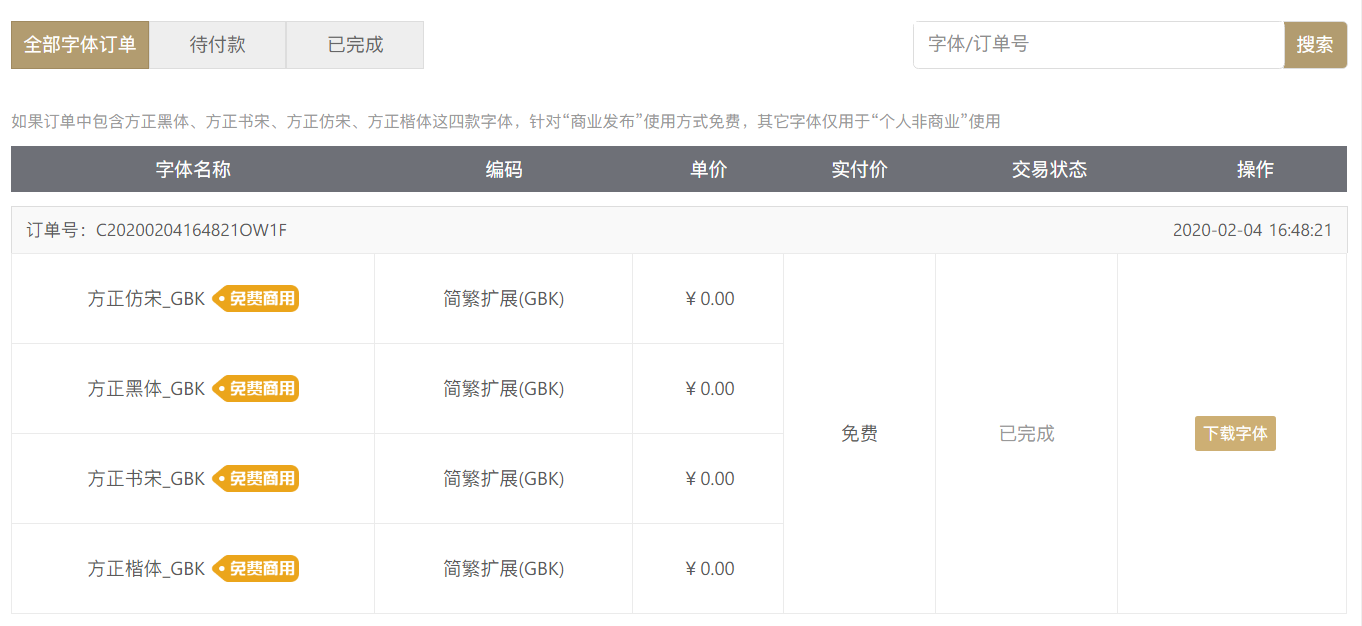
\includegraphics[width=0.9\textwidth]{founder.png}
\end{figure}

\subsection{其他中文字体}
如果你想完全自定义字体\footnote{这里仍然以方正字体为例。},你可以选择 \lstinline{chinesefont=nofont},然后在导言区设置
\begin{lstlisting}
\setCJKmainfont[BoldFont={FZHei-B01},ItalicFont={FZKai-Z03}]{FZShuSong-Z01}
\setCJKsansfont[BoldFont={FZHei-B01}]{FZKai-Z03}
\setCJKmonofont[BoldFont={FZHei-B01}]{FZFangSong-Z02}
\setCJKfamilyfont{zhsong}{FZShuSong-Z01}
\setCJKfamilyfont{zhhei}{FZHei-B01}
\setCJKfamilyfont{zhkai}[BoldFont={FZHei-B01}]{FZKai-Z03}
\setCJKfamilyfont{zhfs}[BoldFont={FZHei-B01}]{FZFangSong-Z02}
\newcommand*{\songti}{\CJKfamily{zhsong}}
\newcommand*{\heiti}{\CJKfamily{zhhei}}
\newcommand*{\kaishu}{\CJKfamily{zhkai}}
\newcommand*{\fangsong}{\CJKfamily{zhfs}}
\end{lstlisting}

\chapter{ElegantBook 写作示例}

\begin{introduction}
  \item 积分定义~\ref{def:int}
  \item Fubini 定理~\ref{thm:fubi}
  \item 最优性原理~\ref{pro:max}
  \item 柯西列性质~\ref{property:cauchy}
  \item 韦达定理
\end{introduction}

\section{Lebesgue 积分}
在前面各章做了必要的准备后,本章开始介绍新的积分。在 Lebesgue 测度理论的基础上建立了 Lebesgue 积分,其被积函数和积分域更一般,可以对有界函数和无界函数统一处理。正是由于 Lebesgue 积分的这些特点,使得 Lebesgue 积分比 Riemann 积分具有在更一般条件下的极限定理和累次积分交换积分顺序的定理,这使得 Lebesgue 积分不仅在理论上更完善,而且在计算上更灵活有效。

Lebesgue 积分有几种不同的定义方式。我们将采用逐步定义非负简单函数,非负可测函数和一般可测函数积分的方式。

由于现代数学的许多分支如概率论、泛函分析、调和分析等常常用到一般空间上的测度与积分理论,在本章最后一节将介绍一般的测度空间上的积分。

\subsection{积分的定义}

我们将通过三个步骤定义可测函数的积分。首先定义非负简单函数的积分。以下设 $E$ 是 $\mathcal{R}^n$ 中的可测集。

\begin{definition}[可积性] \label{def:int} 
设 $ f(x)=\sum\limits_{i=1}^{k} a_i \chi_{A_i}(x)$ 是 $E$ 上的\textbf{非负简单函数},中文其中 $\{A_1,A_2,\ldots,A_k\}$ 是 $E$ 上的一个可测分割,$a_1,a_2,\ldots,a_k$ 是非负实数。定义 $f$ 在 $E$ 上的积分为 $\int_{a}^b f(x)$
\begin{equation}
   \label{inter}
   \int_{E} f dx = \sum_{i=1}^k a_i m(A_i) \pi \alpha\beta\sigma\gamma\nu\xi\epsilon\varepsilon. \oint_{a}^b\ointop_{a}^b\prod_{i=1}^n
\end{equation}
一般情况下 $0 \leq \int_{E} f dx \leq \infty$。若 $\int_{E} f dx < \infty$,则称 $f$ 在 $E$ 上可积。
\end{definition}

一个自然的问题是,Lebesgue 积分与我们所熟悉的 Riemann 积分有什么联系和区别?在 4.4 在我们将详细讨论 Riemann 积分与 Lebesgue 积分的关系。这里只看一个简单的例子。设 $D(x)$ 是区间 $[0,1]$ 上的 Dirichlet 函数。即 $D(x)=\chi_{Q_0}(x)$,其中 $Q_0$ 表示 $[0,1]$ 中的有理数的全体。根据非负简单函数积分的定义,$D(x)$ 在 $[0,1]$ 上的 Lebesgue 积分为
\begin{equation}
   \label{inter2}
   \int_0^1 D(x)dx = \int_0^1 \chi_{Q_0} (x) dx = m(Q_0) = 0
\end{equation}
即 $D(x)$ 在 $[0,1]$ 上是 Lebesgue 可积的并且积分值为零。但 $D(x)$ 在 $[0,1]$ 上不是 Riemann 可积的。


有界变差函数是与单调函数有密切联系的一类函数。有界变差函数可以表示为两个单调递增函数之差。与单调函数一样,有界变差函数几乎处处可导。与单调函数不同,有界变差函数类对线性运算是封闭的,它们构成一线空间。练习题 \ref{exer:43} 是一个性质的证明。

\begin{exercise}\label{exer:43}
设 $f \notin\in L(\mathcal{R}^1)$,$g$ 是 $\mathcal{R}^1$ 上的有界可测函数。证明函数
\begin{equation}
   \label{ex:1}
   I(t) = \int_{\mathcal{R}^1} f(x+t)g(x)dx \quad t \in \mathcal{R}^1
\end{equation}
是 $\mathcal{R}^1$ 上的连续函数。 
\end{exercise}

\begin{solution}
即 $D(x)$ 在 $[0,1]$ 上是 Lebesgue 可积的并且积分值为零。但 $D(x)$ 在 $[0,1]$ 上不是 Riemann 可积的。
\end{solution}

\begin{proof}
即 $D(x)$ 在 $[0,1]$ 上是 Lebesgue 可积的并且积分值为零。但 $D(x)$ 在 $[0,1]$ 上不是 Riemann 可积的。
\end{proof}

\begin{theorem}[Fubini 定理] \label{thm:fubi} 
(1)若 $f(x,y)$ 是 $\mathcal{R}^p\times\mathcal{R}^q$ 上的非负可测函数,则对几乎处处的 $x\in \mathcal{R}^p$,$f(x,y)$ 作为 $y$ 的函数是 $\mathcal{R}^q$ 上的非负可测函数,$g(x)=\int_{\mathcal{R}^q}f(x,y) dy$ 是 $\mathcal{R}^p$ 上的非负可测函数。并且
\begin{equation}
   \label{eq:461}
   \int_{\mathcal{R}^p\times\mathcal{R}^q} f(x,y) dxdy=\int_{\mathcal{R}^p}\left(\int_{\mathcal{R}^q}f(x,y)dy\right)dx.
\end{equation}

(2)若 $f(x,y)$ 是 $\mathcal{R}^p\times\mathcal{R}^q$ 上的可积函数,则对几乎处处的 $x\in\mathcal{R}^p$,$f(x,y)$ 作为 $y$ 的函数是 $\mathcal{R}^q$ 上的可积函数,并且 $g(x)=\int_{\mathcal{R}^q}f(x,y) dy$ 是 $\mathcal{R}^p$ 上的可积函数。而且~\eqref{eq:461} 成立。
\end{theorem}

\begin{note}
在本模板中,引理(lemma),推论(corollary)的样式和定理~\ref{thm:fubi} 的样式一致,包括颜色,仅仅只有计数器的设置不一样。
\end{note}

我们说一个实变或者复变量的实值或者复值函数是在区间上平方可积的,如果其绝对值的平方在该区间上的积分是有限的。所有在勒贝格积分意义下平方可积的可测函数构成一个希尔伯特空间,也就是所谓的 $L^2$ 空间,几乎处处相等的函数归为同一等价类。形式上,$L^2$ 是平方可积函数的空间和几乎处处为 0 的函数空间的商空间。

\begin{proposition}[最优性原理] \label{pro:max}
如果 $u^*$ 在 $[s,T]$ 上为最优解,则 $u^*$ 在 $[s, T]$ 任意子区间都是最优解,假设区间为 $[t_0, t_1]$ 的最优解为 $u^*$ ,则 $u(t_0)=u^{*}(t_0)$,即初始条件必须还是在 $u^*$ 上。
\end{proposition}

我们知道最小二乘法可以用来处理一组数据,可以从一组测定的数据中寻求变量之间的依赖关系,这种函数关系称为经验公式。本课题将介绍最小二乘法的精确定义及如何寻求点与点之间近似成线性关系时的经验公式。假定实验测得变量之间的 $n$ 个数据,则在平面上,可以得到 $n$ 个点,这种图形称为 “散点图”,从图中可以粗略看出这些点大致散落在某直线近旁, 我们认为其近似为一线性函数,下面介绍求解步骤。

\begin{figure}[htbp]
  \centering
  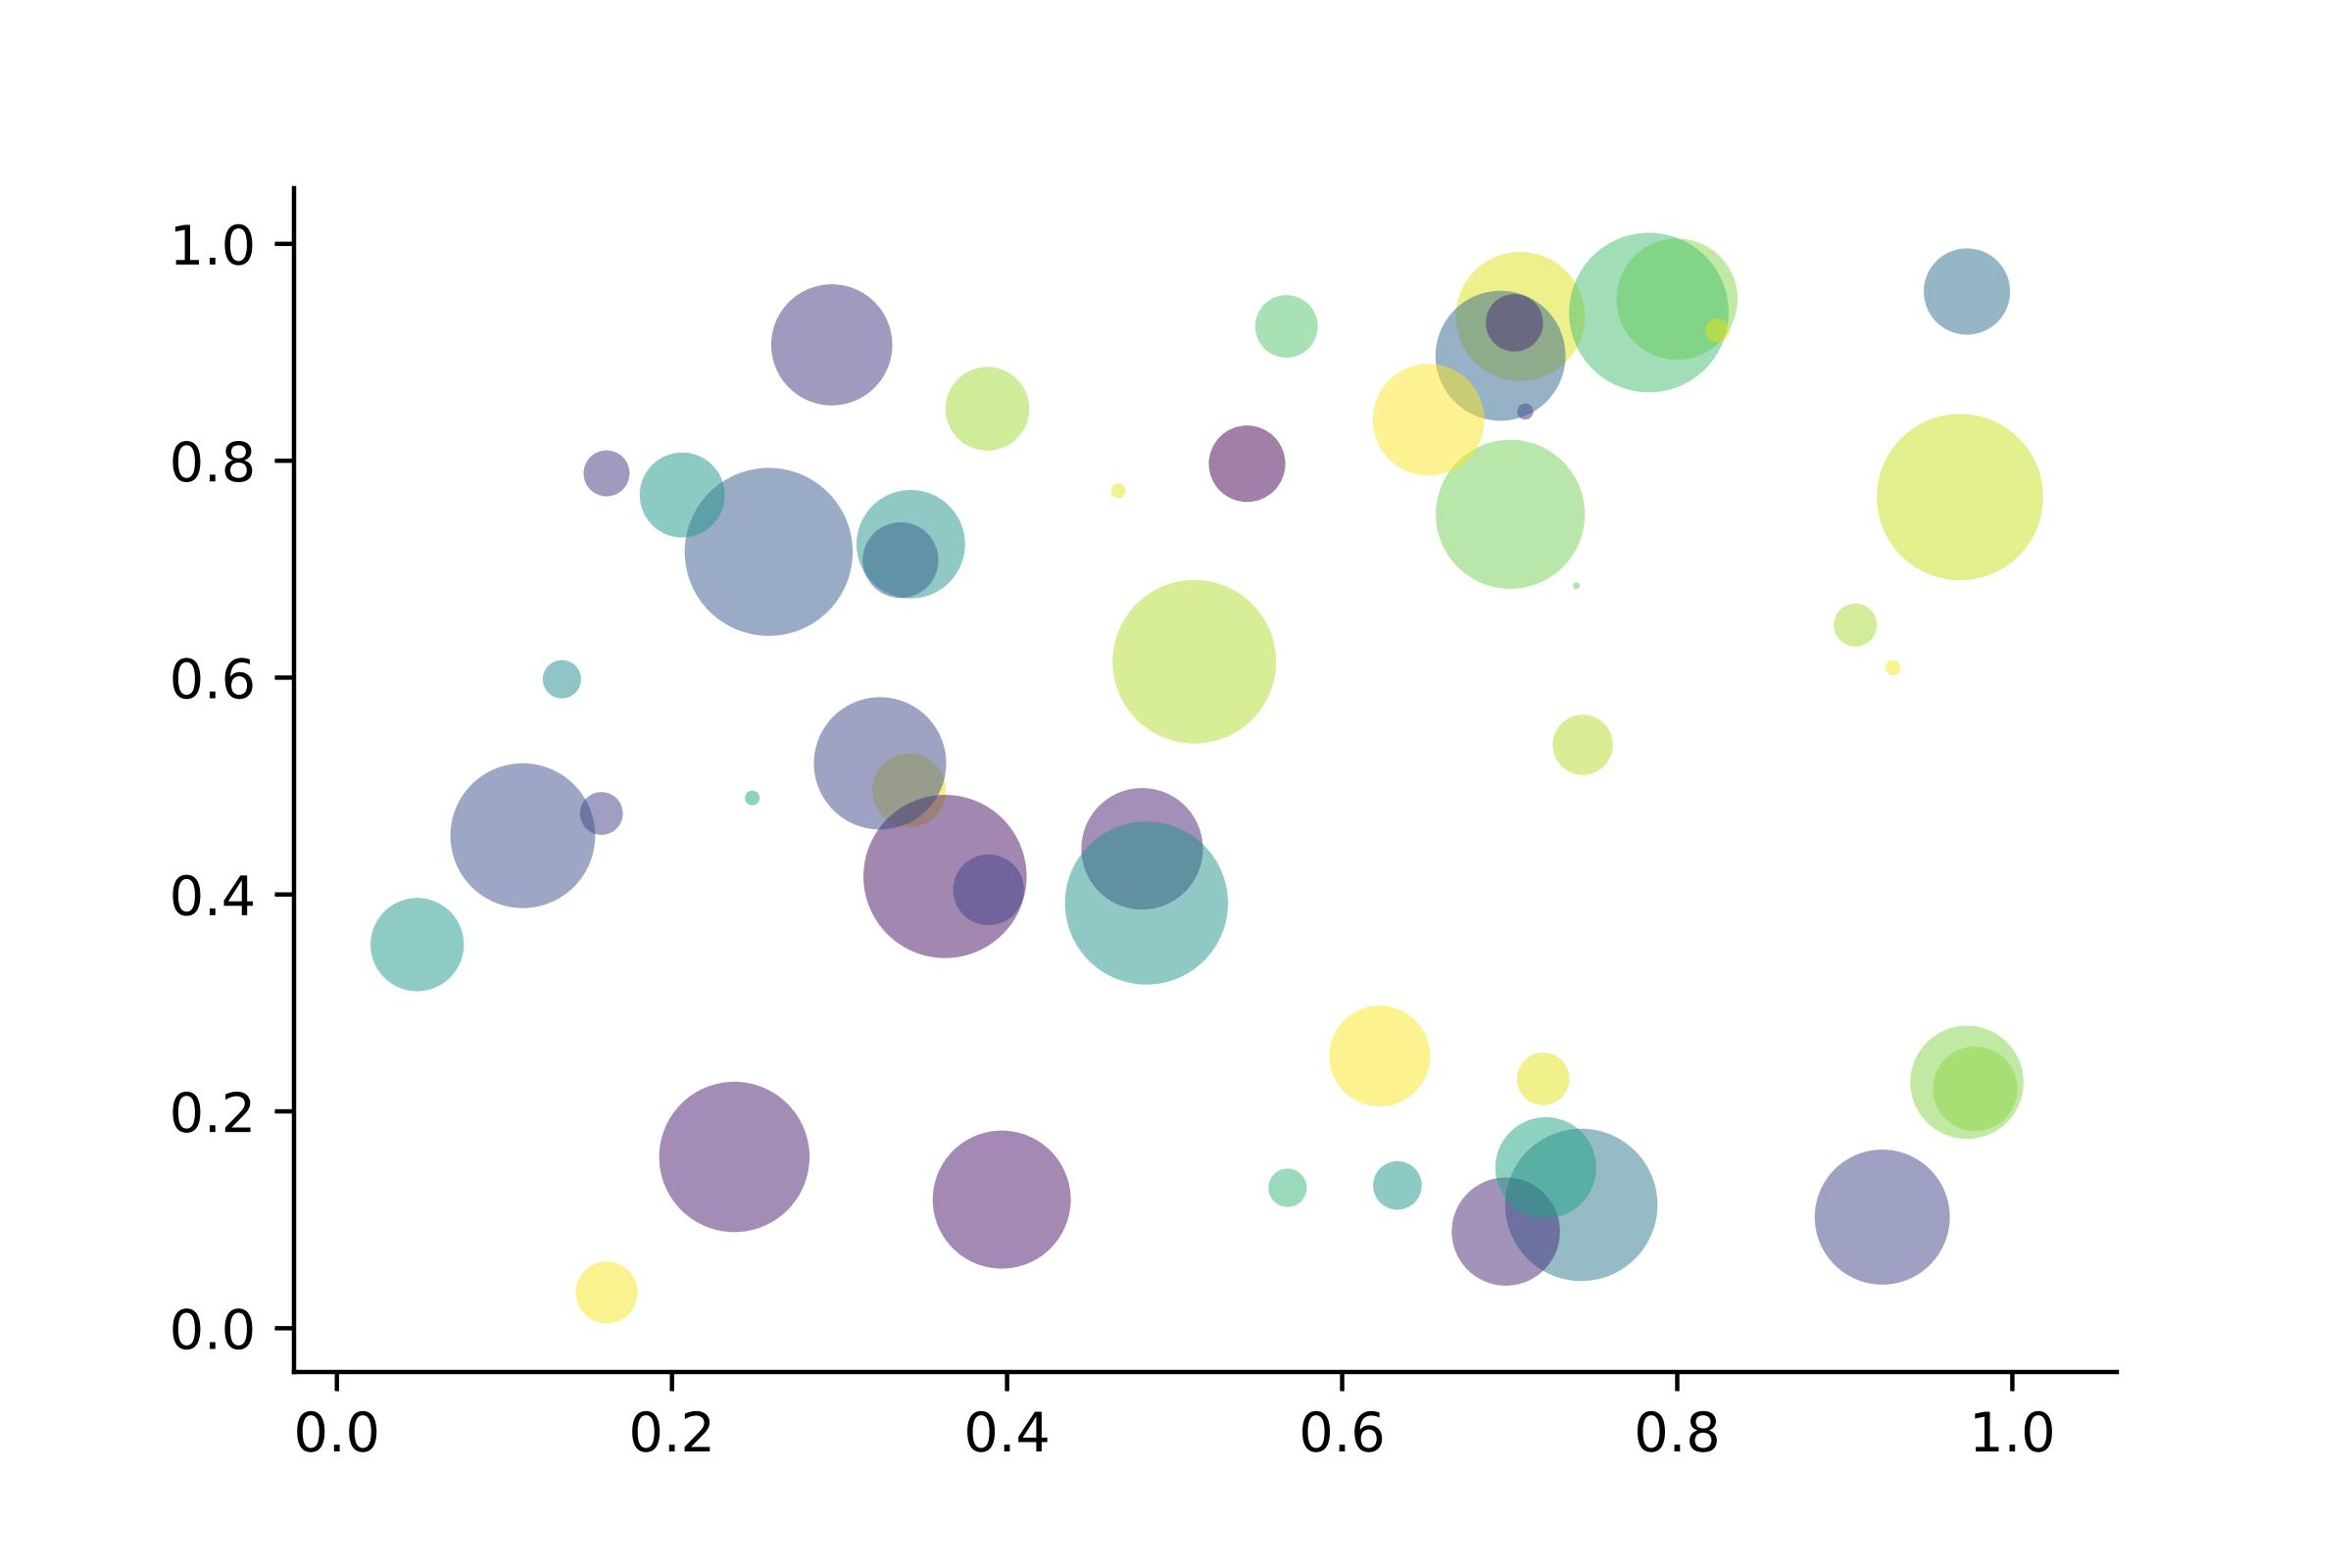
\includegraphics[width=0.6\textwidth]{scatter.jpg}
  \caption{散点图示例 $\hat{y}=a+bx$ \label{fig:scatter}}
\end{figure}

以最简单的一元线性模型来解释最小二乘法。什么是一元线性模型呢?监督学习中,如果预测的变量是离散的,我们称其为分类(如决策树,支持向量机等),如果预测的变量是连续的,我们称其为回归。回归分析中,如果只包括一个自变量和一个因变量,且二者的关系可用一条直线近似表示,这种回归分析称为一元线性回归分析。如果回归分析中包括两个或两个以上的自变量,且因变量和自变量之间是线性关系,则称为多元线性回归分析。对于二维空间线性是一条直线;对于三维空间线性是一个平面,对于多维空间线性是一个超平面。

\begin{property}\label{property:cauchy}
柯西列的性质
\begin{enumerate}
\item $\{x_k\}$ 是柯西列,则其子列 $\{x_k^i\}$ 也是柯西列。
\item $x_k\in \mathcal{R}^n$,$\rho(x,y)$ 是欧几里得空间,则柯西列收敛,$(\mathcal{R}^n,\rho)$ 空间是完备的。
\end{enumerate}
\end{property}

\begin{conclusion}
回归分析(regression analysis) 是确定两种或两种以上变量间相互依赖的定量关系的一种统计分析方法。运用十分广泛,回归分析按照涉及的变量的多少,分为一元回归和多元回归分析;按照因变量的多少,可分为简单回归分析和多重回归分析;按照自变量和因变量之间的关系类型,可分为线性回归分析和非线性回归分析。
\end{conclusion}

\begin{problemset}
\item 设 $A$ 为数域 $K$ 上的 $n$ 级矩阵。证明:如果 $K^n$ 中任意非零列向量都是 $A$ 的特征向量,则 $A$ 一定是数量矩阵。
\item 证明:不为零矩阵的幂零矩阵不能对角化。
\item 设 $A = (a_{ij})$ 是数域 $K$ 上的一个 $n$ 级上三角矩阵,证明:如果 $a_{11} = a_{22} = \cdots = a_{nn}$,并且至少有一个 $a_{kl} \not = 0 (k < l)$,则 $A$ 一定不能对角化。
\end{problemset}

\chapter{常见问题集}

我们根据用户社区反馈整理了下面一些常见的问题,用户在遇到问题时,应当首先查阅本手册和本部分的常见的问题。

\begin{enumerate}[itemsep=1.5ex]
  \item \question{有没有办法章节用“第一章,第一节,(一)”这种?}
    见前文介绍,可以使用 \lstinline{scheme=chinese} 设置。
  \item \question{大佬,我想把正文字体改为亮色,背景色改为黑灰色。}
    页面颜色可以使用 \lstinline{\pagecolor} 命令设置,文本命令可以参考\href{https://tex.stackexchange.com/questions/278544/xcolor-what-is-the-equivalent-of-default-text-color}{这里}进行设置。
  \item \question{\lstinline{! LaTeX Error: Unknown option 'scheme=plain' for package 'ctex'.}}
    你用的 C\TeX{} 套装吧?这个里面的 \lstinline{ctex} 宏包已经是已经是 10 年前的了,与本模板使用的 \lstinline{ctex} 宏集有很大区别。不建议 C\TeX{} 套装了,请卸载并安装 \TeX{} Live 2022。
  \item \question{我该使用什么版本?}
    请务必使用\href{https://github.com/ElegantLaTeX/ElegantBook/releases}{最新正式发行版},发行版间不定期可能会有更新(修复 bug 或者改进之类),如果你在使用过程中没有遇到问题,不需要每次更新\href{https://github.com/ElegantLaTeX/ElegantBook/archive/master.zip}{最新版},但是在发行版更新之后,请尽可能使用最新版(发行版)!最新发行版可以在 GitHub 或者 \TeX{} Live 2021 内获取。
  \item \question{我该使用什么编辑器?}
    你可以使用 \TeX{} Live 2021 自带的编辑器 \TeX{}works 或者使用 \TeX{}studio,\TeX works 的自动补全,你可以参考我们的总结 \href{https://github.com/EthanDeng/texworks-autocomplete}{\TeX works 自动补全}。推荐使用 \TeX{} Live 2021 + \TeX{}studio。我自己用 VS Code 和 Sublime Text,相关的配置说明,请参考 \href{https://github.com/EthanDeng/vscode-latex}{\LaTeX{} 编译环境配置:Visual Studio Code 配置简介} 和 \href{https://github.com/EthanDeng/sublime-text-latex}{Sublime Text 搭建 \LaTeX{} 编写环境}。
  \item \question{您好,我们想用您的 ElegantBook 模板写一本书。关于机器学习的教材,希望获得您的授权,谢谢您的宝贵时间。}
    模板的使用修改都是自由的,你们声明模板来源以及模板地址(GitHub 地址)即可,其他未尽事宜按照开源协议 LPPL-1.3c。做好之后,如果方便的话,可以给我们一个链接,我把你们的教材放在 Elegant\LaTeX{} 用户作品集里。
  \item \question{请问交叉引用是什么?}
    本群和本模板适合有一定 \LaTeX{} 基础的用户使用,新手请先学习 \LaTeX{} 的基础,理解各种概念,否则你将寸步难行。
  \item \question{代码高亮环境能用其他语言吗?}
    可以的,ElegantBook 模板用的是 \lstinline{listings} 宏包,你可以在环境(\lstinline{lstlisting})之后加上语言(比如 Python 使用 \lstinline{language=Python} 选项),全局语言修改请使用 \lstinline{lstset} 命令,更多信息请参考宏包文档。
  \item \question{群主,什么时候出 Beamer 的模板(主题),ElegantSlide 或者 ElegantBeamer?}
    由于 Beamer 中有一个很优秀的主题 \href{https://github.com/matze/mtheme}{Metropolis}。后续确定不会再出任何主题/模板,请大家根据需要修改已有主题。
\end{enumerate}

\chapter{版本更新历史}

根据用户的反馈,我们不断修正和完善模板。由于 3.00 之前版本与现在版本差异非常大,在此不列出 3.00 之前的更新内容。

\datechange{2022/12/31}{版本 4.5} \textcolor{red}{\bfseries 停止维护!}

\datechange{2022/08/17}{版本 4.5 pre}
\begin{change}
  \item \textbf{重要改动}:提供了一个新的文档类选项 \lstinline|usesamecnt|,可以使全局的定理类环境使用同一个计数器。
  \item \textbf{重要改动}:修改了 \lstinline|\elegantnewtheorem| 命令,使其有第五个(可选)参数。
\end{change}

\datechange{2022/08/15}{版本 4.4 正式发布。}

\begin{change}
  \item \textbf{重要改动}:提供了一个定义定理类环境的命令 \lstinline|\elegantnewtheorem|;
  \item \textbf{重要改动}:为所有内置定理类环境提供了带星号的版本,带星号的定理类环境不会编号,修复 \href{https://github.com/ElegantLaTeX/ElegantBook/issues/167}{issue: \#167};
  \item \textbf{重要改动}:在 \lstinline{scheme=chinese} 下将目录中的“第 1 章”修改为“第一章”;
  \item 将 TeX Gyre Termes 改为 TeX Gyre TermesX,使英文部分字形与 newtx 系列宏包更相近;
  \item 重写了内置定理类环境的实现方法,修复了一些 bug,由于修改部分较大,如果引入了新的 bug,请及时在 QQ 群或 \href{https://github.com/ElegantLaTeX}{Github} 上进行反馈;
  \item 删除 Gitee 仓库地址,恢复 GitHub 提交(pull requests);
  \item 将参考文献命令添加到导言区,使编辑器能够对参考文献自动补全。
\end{change}

\datechange{2022/04/09}{版本 4.3 正式发布。}

\begin{change}
  \item 放弃 newtx 系列宏包的设置,改用 TeX Gyre Termes,并设置其他字体;
  \item 修改定理类环境内部字体设置,修复环境内部中文无法加粗问题;
  \item 增加定理类环境的计数器选项 \lstinline{thmcnt},可选 \lstinline{chapter} 和 \lstinline{section};
  \item 增加 \lstinline{bibend} 选项,可选 \lstinline{bibend=biber}(默认)和 \lstinline{bibend=bibtex}。
\end{change}



\datechange{2022/03/08}{版本 4.2 正式发布。}

\begin{change}
  \item 对于 newtx 系列宏包更新导致的字体 bug 的修复;
  \item 修缮目录格式,为了达到这个目的,重新改写 \lstinline{\chaptername} 的重定义语句;
  \item 增加日语 \lstinline{lang=jp} 设定。
  \item 这个版本为一个临时性版本,在 \TeX Live 2022 发布之后,将尽快发布 4.3 版本,由于对于中文的改动比较大,可能会出现预期之外的 bug,有问题可以在 QQ 群或者 Github 反馈。
\end{change}


\datechange{2021/05/02}{版本 4.1 正式发布。}

\begin{change}
  \item \textbf{重要改动}:由原先的 \hologo{BibTeX} 改为 biblatex 编译方式(后端为 \lstinline{biber}),请注意两者之间的差异;
  \item \textbf{重要改进}:修改对于定理写法兼容方式,提高数学公式代码的兼容性;
  \item 页面设置改动,默认页面更宽;方便书写和阅读;
  \item 支持目录文字以及页码跳转;
  \item 不再维护 \hologo{pdfLaTeX} 中文支持方式,请务必使用 \hologo{XeLaTeX} 编译中文文稿。
  \item 增加多个语言选项,法语 \lstinline{lang=fr}、荷兰语 \lstinline{lang=nl}、匈牙利语 \lstinline{lang=hu}、西班牙语 \lstinline{lang=es}、蒙古语 \lstinline{lang=mn} 等。
\end{change}


\datechange{2020/04/12}{版本 3.11 正式发布,\textcolor{red}{此版本为 3.x 最后版本。}}

\begin{change}
  \item \textbf{重要修正}:修复因为 \lstinline{gbt7714} 宏包更新导致的 \lstinline{natbib option clash} 错误;
  \item 由于 \lstinline{pgfornament} 宏包未被 \TeX{} Live 2020 收录,因此删除 base 相关的内容;
  \item 修复部分环境的空格问题;
  \item 增加了意大利语言选项 \lstinline{lang=it}。
\end{change}


\datechange{2020/02/10}{版本 3.10 正式发布}

\begin{change}
  \item 增加数学字体选项 \lstinline{math},可选项为 \lstinline{newtx} 和 \lstinline{cm}。\\
  \textbf{重要提示}:原先通过 \lstinline{newtxmath} 宏包设置的数学字体改为 \LaTeX{} 默认数学字体,如果需要保持原来的字体,需要显式声明数学字体(\lstinline{math=newtx});
  \item 新增中文字体选项 \lstinline{chinesefont},可选项为 \lstinline{ctexfont}、\lstinline{founder} 和 \lstinline{nofont}。
  \item 将封面作者信息设置为可选,并且增加自定义信息命令 \lstinline{\bioinfo};
  \item 在说明文档中增加版本历史,新增 \lstinline{\datechange} 命令和 \lstinline{change} 环境;
  \item 增加汉化章节选项 \lstinline{scheme},可选项为汉化 \lstinline{chinese};
  \item 由于 \lstinline{\lvert} 问题已经修复,重新调整 \lstinline{ctex} 宏包和 \lstinline{amsmath} 宏包位置。
  \item 修改页眉设置,去除了 \lstinline{\lastpage} 以避免 page anchor 问题,加入 \lstinline{\frontmatter}。
  \item 修改参考文献选项 \lstinline{cite},可选项为数字 \lstinline{numbers}、 作者-年份 \lstinline{authoryear} 以及上标 \lstinline{super}。
  \item 新增参考文献样式选项 \lstinline{bibstyle},并将英文模式下参考文献样式 \lstinline{apalike} 设置为默认值,中文仍然使用 \lstinline{gbt7714} 宏包设置。
\end{change}

\datechange{2019/08/18}{版本 3.09 正式发布}

\begin{change}
  \item \lstinline{\elegantpar} 存在 bug,删除 \lstinline{\elegantpar} 命令,建议用户改用 \lstinline{\marginnote} 和 \lstinline{\marginpar} 旁注命令。
  \item 积分操作符统一更改为 \lstinline{esint} 宏包设置;
  \item 新增目录选项 \lstinline{toc},可选项为单栏 \lstinline{onecol} 和双栏 \lstinline{twocol};
  \item 手动增加参考文献选项 \lstinline{cite},可选项为上标形式 \lstinline{super};
  \item 修正章节习题(\lstinline{problemset})环境。
\end{change}

\datechange{2019/05/28}{版本 3.08 正式发布}

\begin{change}
  \item 修复 \lstinline{\part} 命令。
  \item 引入 Note 模板中的 \lstinline{pad} 选项 \lstinline{device=pad}。
  \item 数学字体加入 \lstinline{mtpro2} 可选项 \lstinline{math=mtpro2},使用免费的 \lstinline{lite} 子集。
  \item 将参考文献默认显示方式 \lstinline{authoyear} 改为 \lstinline{numbers}。
  \item 引入旁注命令 \lstinline{\marginpar}(测试)。
  \item 新增章节摘要环境 \lstinline{introduction}。
  \item 新增章节习题环境 \lstinline{problemset}。
  \item 将 \lstinline{\equote} 重命名为 \lstinline{\extrainfo}。
  \item 完善说明文档,增加致谢部分。
\end{change}

\datechange{2019/04/15}{版本 3.07 正式发布}

\begin{change}
  \item 删除中英文自定义字体总设置。
  \item 新增颜色主题,并将原绿色默认主题设置为蓝色 \lstinline{color=blue}。
  \item 引入隐藏装饰图案选项 \lstinline{base},可选项有显示 \lstinline{show} 和隐藏 \lstinline{hide}。
  \item 新增定理模式 \lstinline{mode},可选项有简单模式 \lstinline{simple} 和炫彩模式 \lstinline{fancy}。
  \item 新增隐藏证明、答案等环境的选项 \lstinline{result=noanswer}。
\end{change}

\datechange{2019/02/25}{版本 3.06 正式发布}

\begin{change}
  \item 删除水印。
  \item 新封面,新装饰图案。
  \item 添加引言使用说明。
  \item 修复双面 \lstinline{twoside}。
  \item 美化列表环境。
  \item 增加 \lstinline{\subsubsection} 的设置。
  \item 将模板拆分成中英文语言模式。
  \item 使用 \lstinline{lstlisting} 添加代码高亮。
  \item 增加定理类环境使用说明。
\end{change}

\datechange{2019/01/22}{版本 3.05 正式发布}

\begin{change}
  \item 添加 \lstinline{xeCJK} 宏包中文支持方案。
  \item 修复模板之前对 Ti\textit{k}Z 单位的改动。
  \item 更新 logo 图。
\end{change}

\datechange{2019/01/15}{版本 3.04 正式发布}

\begin{change}
  \item 格式化模板代码。
  \item 增加 \lstinline{\equote} 命令。
  \item 修改 \lstinline{\date}。
\end{change}

\datechange{2019/01/08}{版本 3.03 正式发布}

\begin{change}
  \item 修复附录章节显示问题。
  \item 小幅优化封面代码。
\end{change}

\datechange{2018/12/31}{版本 3.02 正式发布}

\begin{change}
  \item 修复名字系列命令自定义格式时出现的空格问题,比如 \lstinline{\listfigurename}。
  \item 英文定理类名字改为中文名。
  \item 英文结构名改为中文。
\end{change}

\datechange{2018/12/16}{版本 3.01 正式发布}

\begin{change}
  \item 调整 \lstinline{ctex} 宏包。
  \item 说明文档增加更新内容。
\end{change}

\datechange{2018/12/06}{版本 3.00 正式发布}

\begin{change}
  \item 删除 \lstinline{mathpazo} 数学字体选项。
  \item 添加邮箱命令 \lstinline{\mailto}。
  \item 修改英文字体为 \lstinline{newtx} 系列,另外大型操作符号维持 cm 字体。
  \item 中文字体改用 \lstinline{ctex} 宏包自动设置。
  \item 删除 \lstinline{xeCJK} 字体设置,原因是不同系统字体不方便统一。
  \item 定理换用 \lstinline{tcolorbox} 宏包定义,并基本维持原有的定理样式,优化显示效果,支持跨页;定理类名字重命名,如 etheorem 改为 theorem 等等。
  \item 删去自定义的缩进命令 \lstinline{\Eindent}。
  \item 添加参考文献宏包 \lstinline{natbib}。
  \item 颜色名字重命名。
\end{change}

\nocite{*}

\printbibliography[heading=bibintoc, title=\ebibname]
\appendix

\chapter{基本数学工具}


本附录包括了计量经济学中用到的一些基本数学,我们扼要论述了求和算子的各种性质,研究了线性和某些非线性方程的性质,并复习了比例和百分数。我们还介绍了一些在应用计量经济学中常见的特殊函数,包括二次函数和自然对数,前 4 节只要求基本的代数技巧,第 5 节则对微分学进行了简要回顾;虽然要理解本书的大部分内容,微积分并非必需,但在一些章末附录和第 3 篇某些高深专题中,我们还是用到了微积分。

\section{求和算子与描述统计量}

\textbf{求和算子} 是用以表达多个数求和运算的一个缩略符号,它在统计学和计量经济学分析中扮演着重要作用。如果 $\{x_i: i=1, 2, \ldots, n\}$ 表示 $n$ 个数的一个序列,那么我们就把这 $n$ 个数的和写为:

\begin{equation}
\sum_{i=1}^n x_i \equiv x_1 + x_2 +\cdots + x_n
\end{equation}



\end{document}
